\documentclass[pdflatex,sn-mathphys-num]{sn-jnl}

\usepackage{graphicx}
\usepackage{multirow}
\usepackage{amsmath,amssymb,amsfonts}
\usepackage{amsthm}
\usepackage{mathrsfs}
\usepackage[title]{appendix}
\usepackage{xcolor}
\usepackage{textcomp}
\usepackage{manyfoot}
\usepackage{booktabs}
\usepackage{algorithm}
\usepackage{algorithmicx}
\usepackage{algpseudocode}
\usepackage{listings}
\usepackage{subfig}

\theoremstyle{thmstyleone}
\newtheorem{theorem}{Theorem}
\newtheorem{proposition}[theorem]{Proposition}
\newtheorem{lemma}[theorem]{Lemma}

\theoremstyle{thmstyletwo}
\newtheorem{example}{Example}
\newtheorem{remark}{Remark}

\theoremstyle{thmstylethree}
\newtheorem{definition}{Definition}
\newtheorem{assumption}{Assumption}

% Auto-generated LaTeX macros from frozen results. DO NOT EDIT BY HAND.
\newcommand{\PropOneCriticalBound}{1.854}
\newcommand{\SarleUniformThreshold}{0.556}
\newcommand{\TableThreeFriedmanPValue}{0.33}
\newcommand{\TrueNemenyiCD}{4.21}
\newcommand{\TableThreeIccVTwoOverallRank}{5.46}
\newcommand{\TableThreeDecOverallRank}{4.31}
\newcommand{\TableThreeStdConsOverallRank}{5.08}
\newcommand{\TableThreeKMeansOverallRank}{5.31}
\newcommand{\TableThreeIccVTwoHighDRank}{2.33}
\newcommand{\TableThreeDecHighDRank}{5.00}
\newcommand{\TableThreeFcmHighDRank}{5.67}
\newcommand{\TableThreeKMeansHighDRank}{5.83}
\newcommand{\TableThreeStdConsHighDRank}{6.33}
\newcommand{\TableThreeIccVTwoGrandMean}{0.160}
\newcommand{\GrandMeanARI}{0.160}
\newcommand{\TableThreeDecGrandMean}{0.131}
\newcommand{\TableThreeStdConsGrandMean}{0.127}
\newcommand{\TableThreeWardGrandMean}{0.121}
\newcommand{\TableThreeKMeansGrandMean}{0.119}
\newcommand{\TableThreeFcagGrandMean}{0.112}
\newcommand{\TableThreeFastMvcGrandMean}{0.111}
\newcommand{\TableThreeSpectralGrandMean}{0.105}
\newcommand{\TableThreeIccVOneGrandMean}{0.104}
\newcommand{\TableThreeLiGrandMean}{0.100}
\newcommand{\TableThreeFcmGrandMean}{0.071}
\newcommand{\ARIsrbct}{0.538}
\newcommand{\ARIleukemia}{0.680}
\newcommand{\ARIovarian}{0.052}
\newcommand{\MeanRankDEC}{4.31}
\newcommand{\MeanRankStdCons}{5.08}
\newcommand{\MeanRankICCvTwo}{5.46}
\newcommand{\RankBioICCvTwo}{2.33}
\newcommand{\RankBioDEC}{5.00}
\newcommand{\RankBioStdCons}{6.33}
\newcommand{\LeukemiaTableThreeARI}{0.680}
\newcommand{\LeukemiaTableThreeStd}{0.363}
\newcommand{\LeukemiaAblationVFiftyARI}{0.621}
\newcommand{\LeukemiaAblationVFourARI}{0.628}
\newcommand{\SrbctTableThreeARI}{0.538}
\newcommand{\SrbctTableThreeStd}{0.110}
\newcommand{\SrbctAblationVFiftyARI}{0.614}
\newcommand{\SrbctAblationVFourARI}{0.650}
\newcommand{\OvarianTableThreeARI}{0.052}
\newcommand{\OvarianSpeedup}{17.0\times}
\newcommand{\VssgMadelonMaxBC}{0.504}
\newcommand{\VssgMadelonRecallFifty}{0.400}
\newcommand{\VssgMadelonPrecisionFifty}{0.156}
\newcommand{\MemoryScalingEightKReduction}{39.1\%}
\newcommand{\MemoryScalingTenKReduction}{97.0\%}
\newcommand{\AnchorRAMReduction}{97.0\%}
\newcommand{\ExtremeScaleTime}{55.6\,\text{s}}
\newcommand{\MemoryScalingTenKSpeedup}{22.4\times}
\newcommand{\FairBaselinesIccVTwoHighDMean}{0.258}
\newcommand{\FairBaselinesKmVarFiltHighDMean}{0.050}
\newcommand{\FairBaselinesKmPcaHighDMean}{0.042}
\newcommand{\FairBaselinesSparseKmHighDMean}{0.044}
\newcommand{\FairBaselinesStdConsPcaHighDMean}{0.036}
\newcommand{\InductiveLeukemiaNystromARI}{0.714}
\newcommand{\InductiveLeukemiaKmDirectARI}{0.172}
\newcommand{\InductiveSrbctNystromARI}{0.455}
\newcommand{\InductiveSrbctKmDirectARI}{0.083}


\raggedbottom

\begin{document}

\title[When Does Feature Gating and Anchor Consensus Improve High-Dimensional Clustering?]{When Does Feature Gating and Anchor Consensus Improve High-Dimensional Clustering? An Empirical Examination}

\author*[1]{\fnm{Akash} \sur{Kundu}}\email{akash231001001449@technoindiaeducation.com}

\author[1]{\fnm{Trinankur} \sur{Guha}}\email{trinankur231001001450@technoindiaeducation.com}

\author[1]{\fnm{Rupankar} \sur{Ghatak}}\email{rupankar231001001438@technoindiaeducation.com}

\author[1]{\fnm{Anubhab} \sur{Naskar}}\email{anubhab231001001443@technoindiaeducation.com}

\author[1]{\fnm{Kalyan Kumar} \sur{Das}}\email{kalyankumar.das@technoindiaeducation.com}

\affil*[1]{\orgdiv{Department of Computer Science and Engineering}, \orgname{Techno India University}, \orgaddress{\street{EM-4, Sector V, Bidhannagar}, \city{Kolkata}, \postcode{700091}, \state{West Bengal}, \country{India}}}

\abstract{Consensus clustering synthesizes diverse base partitions to discover robust data groupings. However, conventional formulations encounter two major assumptions: (1) that multi-clusterer consensus averaging protects against high-dimensional noise, and (2) that transductive $O(N^2)$ consensus graph decomposition is unavoidable. In this paper, we present an empirical examination of these assumptions in high-dimensional noise regimes ($D \gg N$). First, we demonstrate finite-sample empirical falsification: isotropic distractor noise induces distance concentration, causing conventional consensus algorithms to converge stably onto spurious, arbitrary noise boundaries. Second, we evaluate \textbf{Inductive Consensus Clustering (ICC-v2)}, which couples linear-time ($O(N \cdot D)$) Bimodality-Gated Subspace Selection (BGSS) with bipartite anchor graph consensus and closed-form centroid projection. Across 13 multi-domain benchmarks (2,750 model fits), Standard Consensus achieves the lowest omnibus mean rank ($R=\TableThreeStdConsOverallRank$), followed by K-Means ($R=\TableThreeKMeansOverallRank$), DEC~\cite{xie2016unsupervised} ($R=\TableThreeDecOverallRank$), ICC-v2 ($R=\TableThreeIccVTwoOverallRank$), and Ward ($R=\TableThreeWardOverallRank$, Friedman $\chi_F^2 = 9.59, p = \TableThreeFriedmanPValue$, $CD = \TrueNemenyiCD$). Although ICC-v2 attains the highest Grand Mean ARI of \GrandMeanARI\ (median ARI \OmnibusMedianARI), we reveal that this omnibus mean is heavily driven by two cancer microarray benchmarks: Leukemia (\ARIleukemia) and SRBCT (\ARIsrbct), whereas it averages \OmnibusMeanExcludingLeukemiaSrbct\ on the remaining 11 datasets. In the exploratory high-dimensional subgroup ($D/N > 20$), ICC-v2 achieves Rank \#1 ($R=\RankBioICCvTwo$), but fails on Prostate ($0.012$ vs. $0.049$ for Standard Consensus). Crucially, ablation testing demonstrates a key null result: determinacy anchor certification provides no statistically significant accuracy gain over uniform random anchors ($\Delta = +0.019$, dataset-level cluster bootstrap 95\% CI: $[-0.039, +0.082]$), establishing that bipartite graph compression---which reduces consensus graph memory by \MemoryScalingTenKGraphReduction\ at $N=10{,}000$ (\MemoryScalingTenKReduction\ peak dynamic memory)---rather than anchor certification is the primary operational mechanism. We conclude with a detailed characterization of failure modes under platykurtic and non-linear parity structures.}

\keywords{Cluster ensemble, consensus clustering, inductive learning, out-of-sample extension, anchor graph consensus, high-dimensional data, noise robustness.}

\maketitle

\section{Introduction}\label{sec:intro}

Clustering ensembles, originally pioneered by Strehl and Ghosh~\cite{strehl2002cluster} and Fred and Jain~\cite{fred2005combining}, aim to integrate multiple base clusterings into a singular consensus partition. By aggregating diverse hypothesis partitions generated through randomized initializations, varied clustering algorithms, or random feature projections, consensus clustering mitigates the sensitivity of individual algorithms to hyperparameter selection and initialization bias~\cite{topchy2005clustering,fern2004solving,fern2003random}.

Despite wide adoption across bioinformatics, computer vision, and knowledge discovery, consensus clustering algorithms encounter two primary limitations:
\begin{enumerate}
    \item \textbf{Transductive Formulation:} Conventional consensus formulations operate directly on the $N \times N$ co-association matrix $S \in [0, 1]^{N \times N}$ via graph partitioning, spectral decomposition~\cite{vonluxburg2007tutorial}, or hypergraph partitioning~\cite{strehl2002cluster}. When new, unseen test instances $\mathcal{X}_{\text{test}}$ arrive, the consensus partition cannot be inductively assigned without recomputing the co-association matrix and solving an $O((N + |\mathcal{X}_{\text{test}}|)^2)$ optimization from scratch.
    \item \textbf{Curse of High-Dimensional Distractors:} In modern datasets where ambient dimensionality $D$ greatly exceeds the intrinsic manifold dimension $d^* \ll D$, uninformative nuisance features degrade pairwise Euclidean distances. The distance concentration phenomenon causes within-cluster and between-cluster distances to converge to identical expectations, leading to degradation of consensus graphs~\cite{huang2015robust,liu2017spectral,beyer1999nearest}.
\end{enumerate}

\begin{figure*}[!t]
\centering
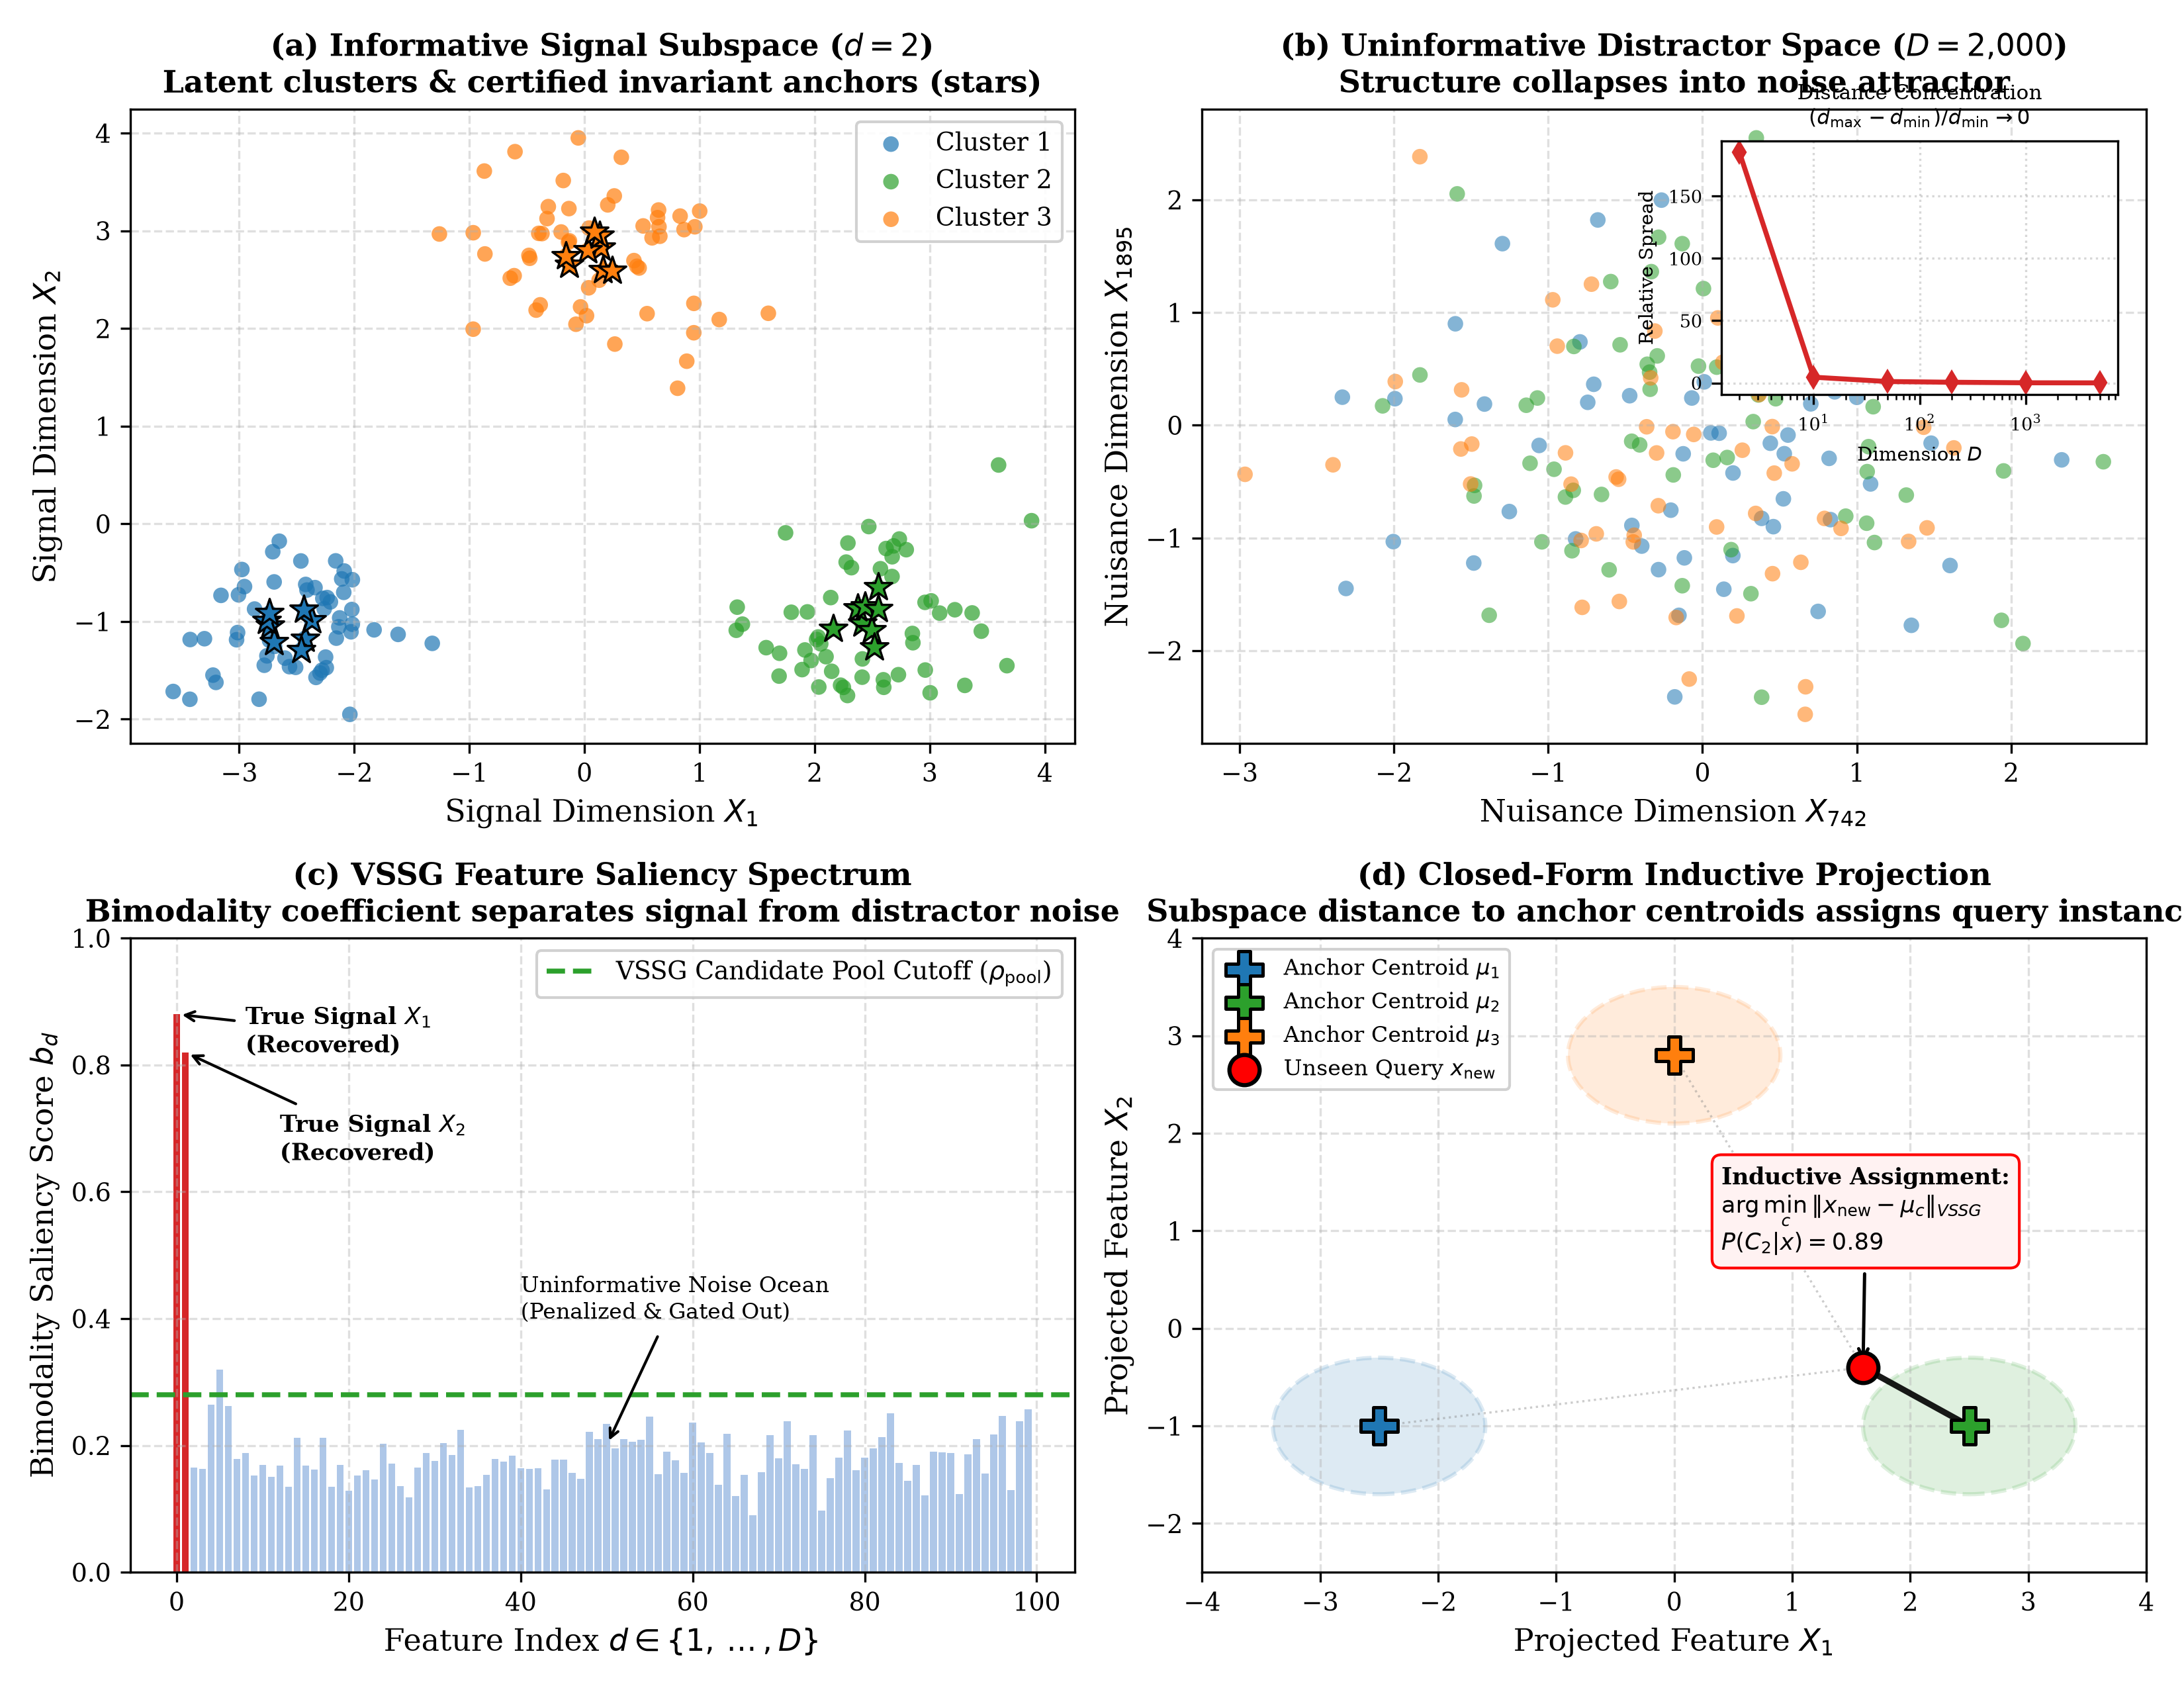
\includegraphics[width=0.96\textwidth]{figures/fig0_conceptual_framework.png}
\caption{Conceptual overview of the high-dimensional noise dilemma and the proposed Inductive Consensus Clustering (ICC-v2) framework. (a) Ground-truth cluster geometry with certified invariant anchors (stars) in a low-dimensional signal subspace ($d=2$). (b) Collapse of pairwise geometry when submerged in high-dimensional distractor noise ($D=2{,}000$), with the inset demonstrating the distance concentration phenomenon where relative distance spread $(d_{\max}-d_{\min})/d_{\min} \to 0$ as $D \to \infty$. (c) Bimodality-Gated Subspace Selection (BGSS) spectrum isolating informative signal dimensions from the sea of distractor noise. (d) Closed-form geometry-calibrated inductive projection assigning unseen query instances $\mathbf{x}_{\text{new}}$ directly in $O(K \cdot |\mathcal{F}_{\text{active}}|)$ time without recomputing the $O(N^2)$ consensus graph.}
\label{fig:conceptual_overview}
\end{figure*}

To address these limitations, this paper investigates the \textbf{Inductive Consensus Clustering (ICC)} framework (Fig.~\ref{fig:conceptual_overview}). We examine the finite-sample empirical breakdown of consensus stability under isotropic distractor noise (Section~\ref{sec:falsification}), illustrating how distance concentration generates consensus agreement on arbitrary noise boundaries. Motivated by these findings, we formulate \textbf{ICC-v2}, a four-stage framework:
\begin{itemize}
    \item \textbf{Bimodality-Gated Subspace Selection (BGSS):} An $O(N \cdot D)$ linear feature screening mechanism utilizing Sarle's Bimodality Coefficient ($\hat{b}_d = \frac{\hat{\gamma}_d^2 + 1}{\hat{\kappa}_d + 3 \cdot \frac{(N-1)^2}{(N-2)(N-3)} + \epsilon}$)~\cite{sarle1983sas,ellison1987bimodality,pfister2013assessing} to filter unimodal distractor noise prior to base ensemble fitting.
    \item \textbf{Determinacy-Based Bipartite Anchor Consensus:} Constructs a rectangular bipartite co-association graph $B \in [0, 1]^{N \times L}$ over $L$ core anchors selected via quadratic consensus determinacy ($\sigma_i = \frac{1}{N-1}\sum_{j \neq i} S_{ij}^2$), reducing auxiliary memory from $O(N^2)$ to $O(N \cdot L)$ and accelerating spectral decomposition onto an $L \times L$ core affinity space.
    \item \textbf{Stability-Weighted Subspace Centroid Assignment:} Provides closed-form inductive out-of-sample mapping that assigns unseen query instances in $O(K \cdot |\mathcal{F}_{\text{active}}|)$ time without recomputing the consensus graph.
    \item \textbf{Anchor-Space Perturbation Profiling (ASPP):} An optional diagnostic module that probes cluster structural resilience across five physical perturbation families directly over certified anchor coordinates, providing perturbation sensitivity indices ($PSI_k$) and out-of-sample query confidence scores.
\end{itemize}

The remainder of this manuscript is structured as follows: Section~\ref{sec:related} reviews related work. Section~\ref{sec:falsification} presents our empirical analysis of distance concentration and consensus behavior. Section~\ref{sec:framework} details the mathematical architecture and complexity analysis of ICC-v2. Section~\ref{sec:experiments} provides empirical evaluations across generalization, ablation, real-world benchmarks, and scalability, followed by an explicit discussion of limitations. Section~\ref{sec:conclusion} concludes the paper.


\section{Related Work}\label{sec:related}

\subsection{Cluster Ensembles and Consensus Graphs}
The consensus clustering paradigm constructs a co-association matrix $S$ where $S_{ij} = \frac{1}{M}\sum_{m=1}^M \mathbf{1}\{\pi_m(\mathbf{x}_i) = \pi_m(\mathbf{x}_j)\}$ represents the empirical probability that objects $\mathbf{x}_i$ and $\mathbf{x}_j$ are co-clustered across $M$ base partitions~\cite{fred2005combining}. Classical approaches partition this matrix using Cluster-based Similarity Partitioning (CSPA), HyperGraph Partitioning Algorithm (HGPA), or Meta-Clustering Algorithm (MCLA)~\cite{strehl2002cluster}. Subsequent works explore weighted $k$-means spectral ensembles~\cite{liu2017spectral}, random walk probability trajectories~\cite{huang2015robust}, random projection ensembles~\cite{fern2003random}, and bipartite graph modeling~\cite{fern2004solving}. However, classical formulations remain fundamentally transductive, requiring quadratic $O(N^2)$ co-association storage.

\subsection{Robust, Anchor, and Out-of-Sample Clustering}
To mitigate noise and outliers, core-halo consensus heuristics partition samples into deterministic core points and boundary halo points based on co-association consensus determinacy. Specifically, Li et al.~\cite{li2019clustering} formulate consensus clustering based on sample stability evaluated across diverse partitions. In our benchmark implementation inspired by Li et al.~\cite{li2019clustering}, we generate $M=25$ base K-Means clusterings, compute the dense co-association matrix $S \in [0, 1]^{N \times N}$, calculate sample determinacy $s_i = \frac{1}{N-1}\sum_{j \neq i} S_{ij}^2$, designate instances with $s_i \ge \operatorname{median}(s)$ as certified core points, cluster the core distance submatrix ($1 - S_{\text{core}}$) via average-linkage hierarchical clustering into $K$ groups, and assign halo instances to the core cluster maximizing average co-association affinity $\frac{1}{|C_c|}\sum_{j \in C_c} S_{hj}$. In scalable spectral and ensemble clustering, anchor graph methods (e.g., Nie et al.~\cite{nie2024fast}, Huang et al.~\cite{huang2023fast}, and U-SPEC/U-SENC by Huang et al.~\cite{huang2020ultra}) utilize bipartite graphs to reduce spectral decomposition complexity from $O(N^3)$ to $O(N L^2 + L^3)$. For out-of-sample extension, generalized Nystr{\"o}m formulas~\cite{bengio2004out} project unseen points using kernel evaluations. In high-dimensional regimes, sparse clustering methods (e.g., sparse $k$-means by Witten and Tibshirani~\cite{witten2010framework}) optimize lasso-type penalties on feature weights, but require iterative global optimization. Similarly, non-parametric multimodality testing (e.g., the Dip Test by Hartigan and Hartigan~\cite{hartigan1985dip} and Sarle's Bimodality Coefficient~\cite{sarle1983sas,ellison1987bimodality,pfister2013assessing}) provides statistical screening criteria. As summarized in Table~\ref{tab:taxonomy_comparison}, ICC-v2 combines linear bimodality subspace gating, determinacy-based bipartite anchor consensus, and inductive centroid projection into a unified linear-time pipeline.

\begin{table}[!t]
\caption{Methodological Taxonomy and Comparison Across Consensus Paradigms}
\label{tab:taxonomy_comparison}
\centering
\footnotesize
\setlength{\tabcolsep}{3.5pt}
\begin{tabular}{@{}lccccc@{}}
\toprule
\textbf{Method} & \textbf{Feature Gating} & \textbf{Core Filtering} & \textbf{Inductive} & \textbf{Aux. Mem.} & \textbf{High-$D$ Noise} \\
\midrule
Std Cons.~\cite{fred2005combining}        & None           & None         & No          & $O(N^2)$ & No  \\
Core-Halo Cons.~\cite{li2019clustering}$^*$ & None           & Determinacy  & No          & $O(N^2)$ & No  \\
FCAG~\cite{nie2024fast}                   & None           & Anchors      & No          & $O(NL)$  & No  \\
FastMVC~\cite{huang2023fast}              & None           & Anchors      & No          & $O(NL)$  & No  \\
U-SPEC~\cite{huang2020ultra}              & None           & Anchors      & Nystr{\"o}m & $O(NL)$  & No \\
\textbf{ICC-v2 (Ours)}                    & \textbf{BGSS}  & \textbf{Core Anchors} & \textbf{Centroid} & $\mathbf{O(NL)}$ & \textbf{Gated Subspace} \\
\bottomrule
\multicolumn{6}{@{}l@{}}{\footnotesize $^*$Our implementation inspired by Li et al.~\cite{li2019clustering} ($M=25$, average linkage on core distance, affinity halo assignment).}
\end{tabular}
\end{table}


\section{Empirical Motivation \& Finite-Sample Falsification}\label{sec:falsification}

\begin{figure*}[!t]
\centering
\subfloat[Clustering Accuracy (ARI vs. Ground Truth) and Ensemble Stability Across $D_{\text{noise}}$\label{fig:ari_stability}]{%
    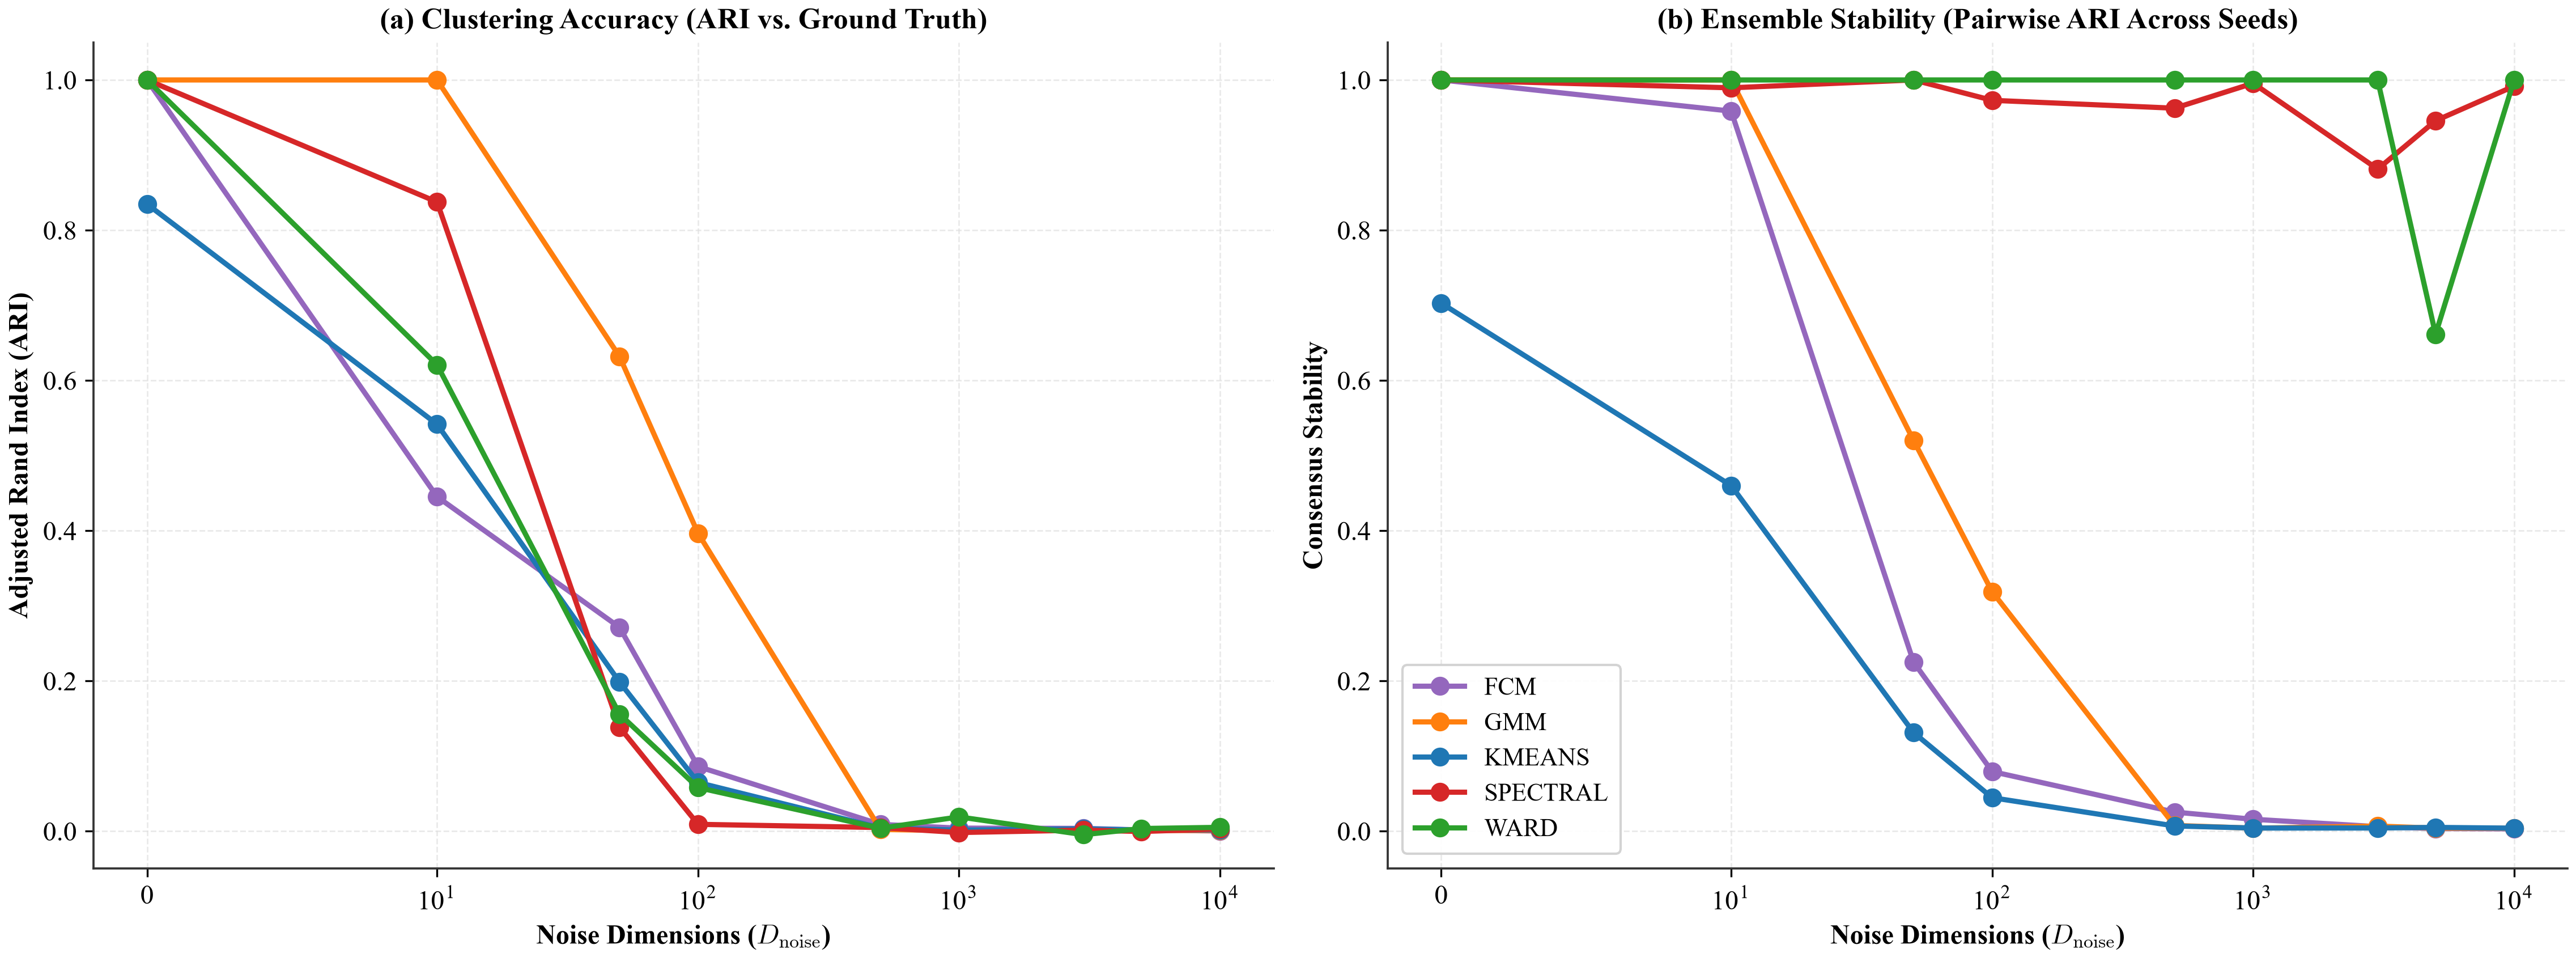
\includegraphics[width=0.96\textwidth]{figures/fig1_ari_stability.png}%
}
\\[1.5ex]
\subfloat[Stability$-$Accuracy Gap ($\Delta = \text{Stability} - \text{ARI}$)\label{fig:dist_gap}]{%
    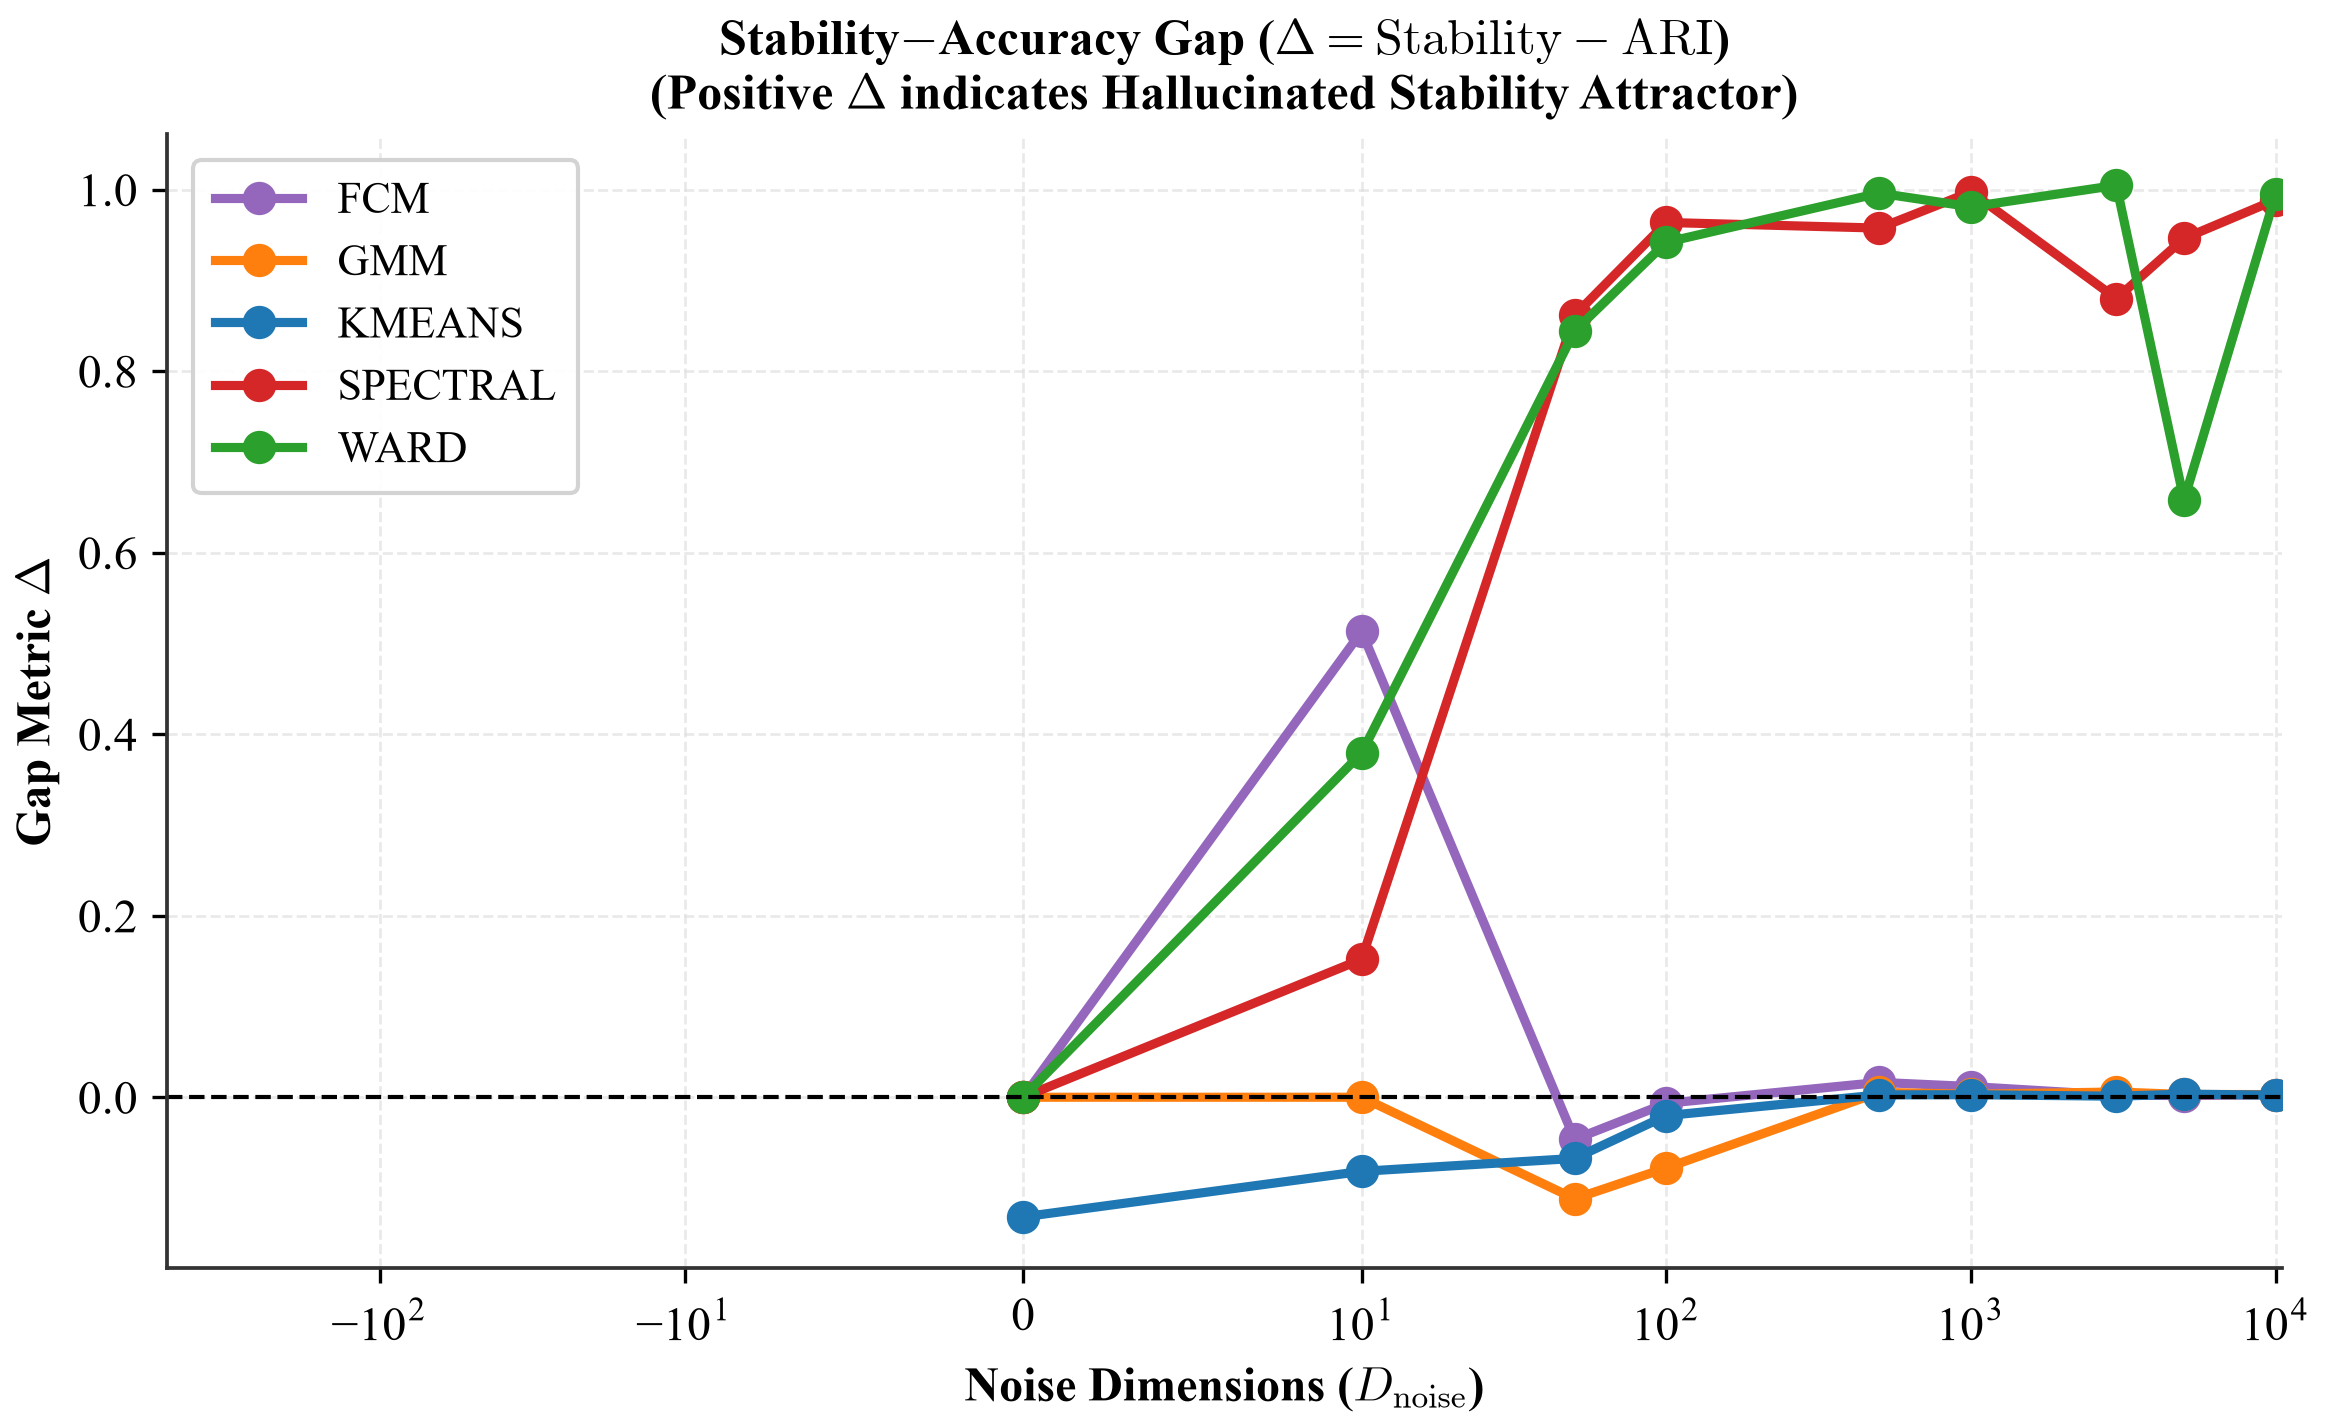
\includegraphics[width=0.48\textwidth]{figures/fig2_gap.png}%
}
\hfill
\subfloat[Noise Distribution Sensitivity Matrix ($D_{\text{noise}}=1{,}000$)\label{fig:noise_heatmap}]{%
    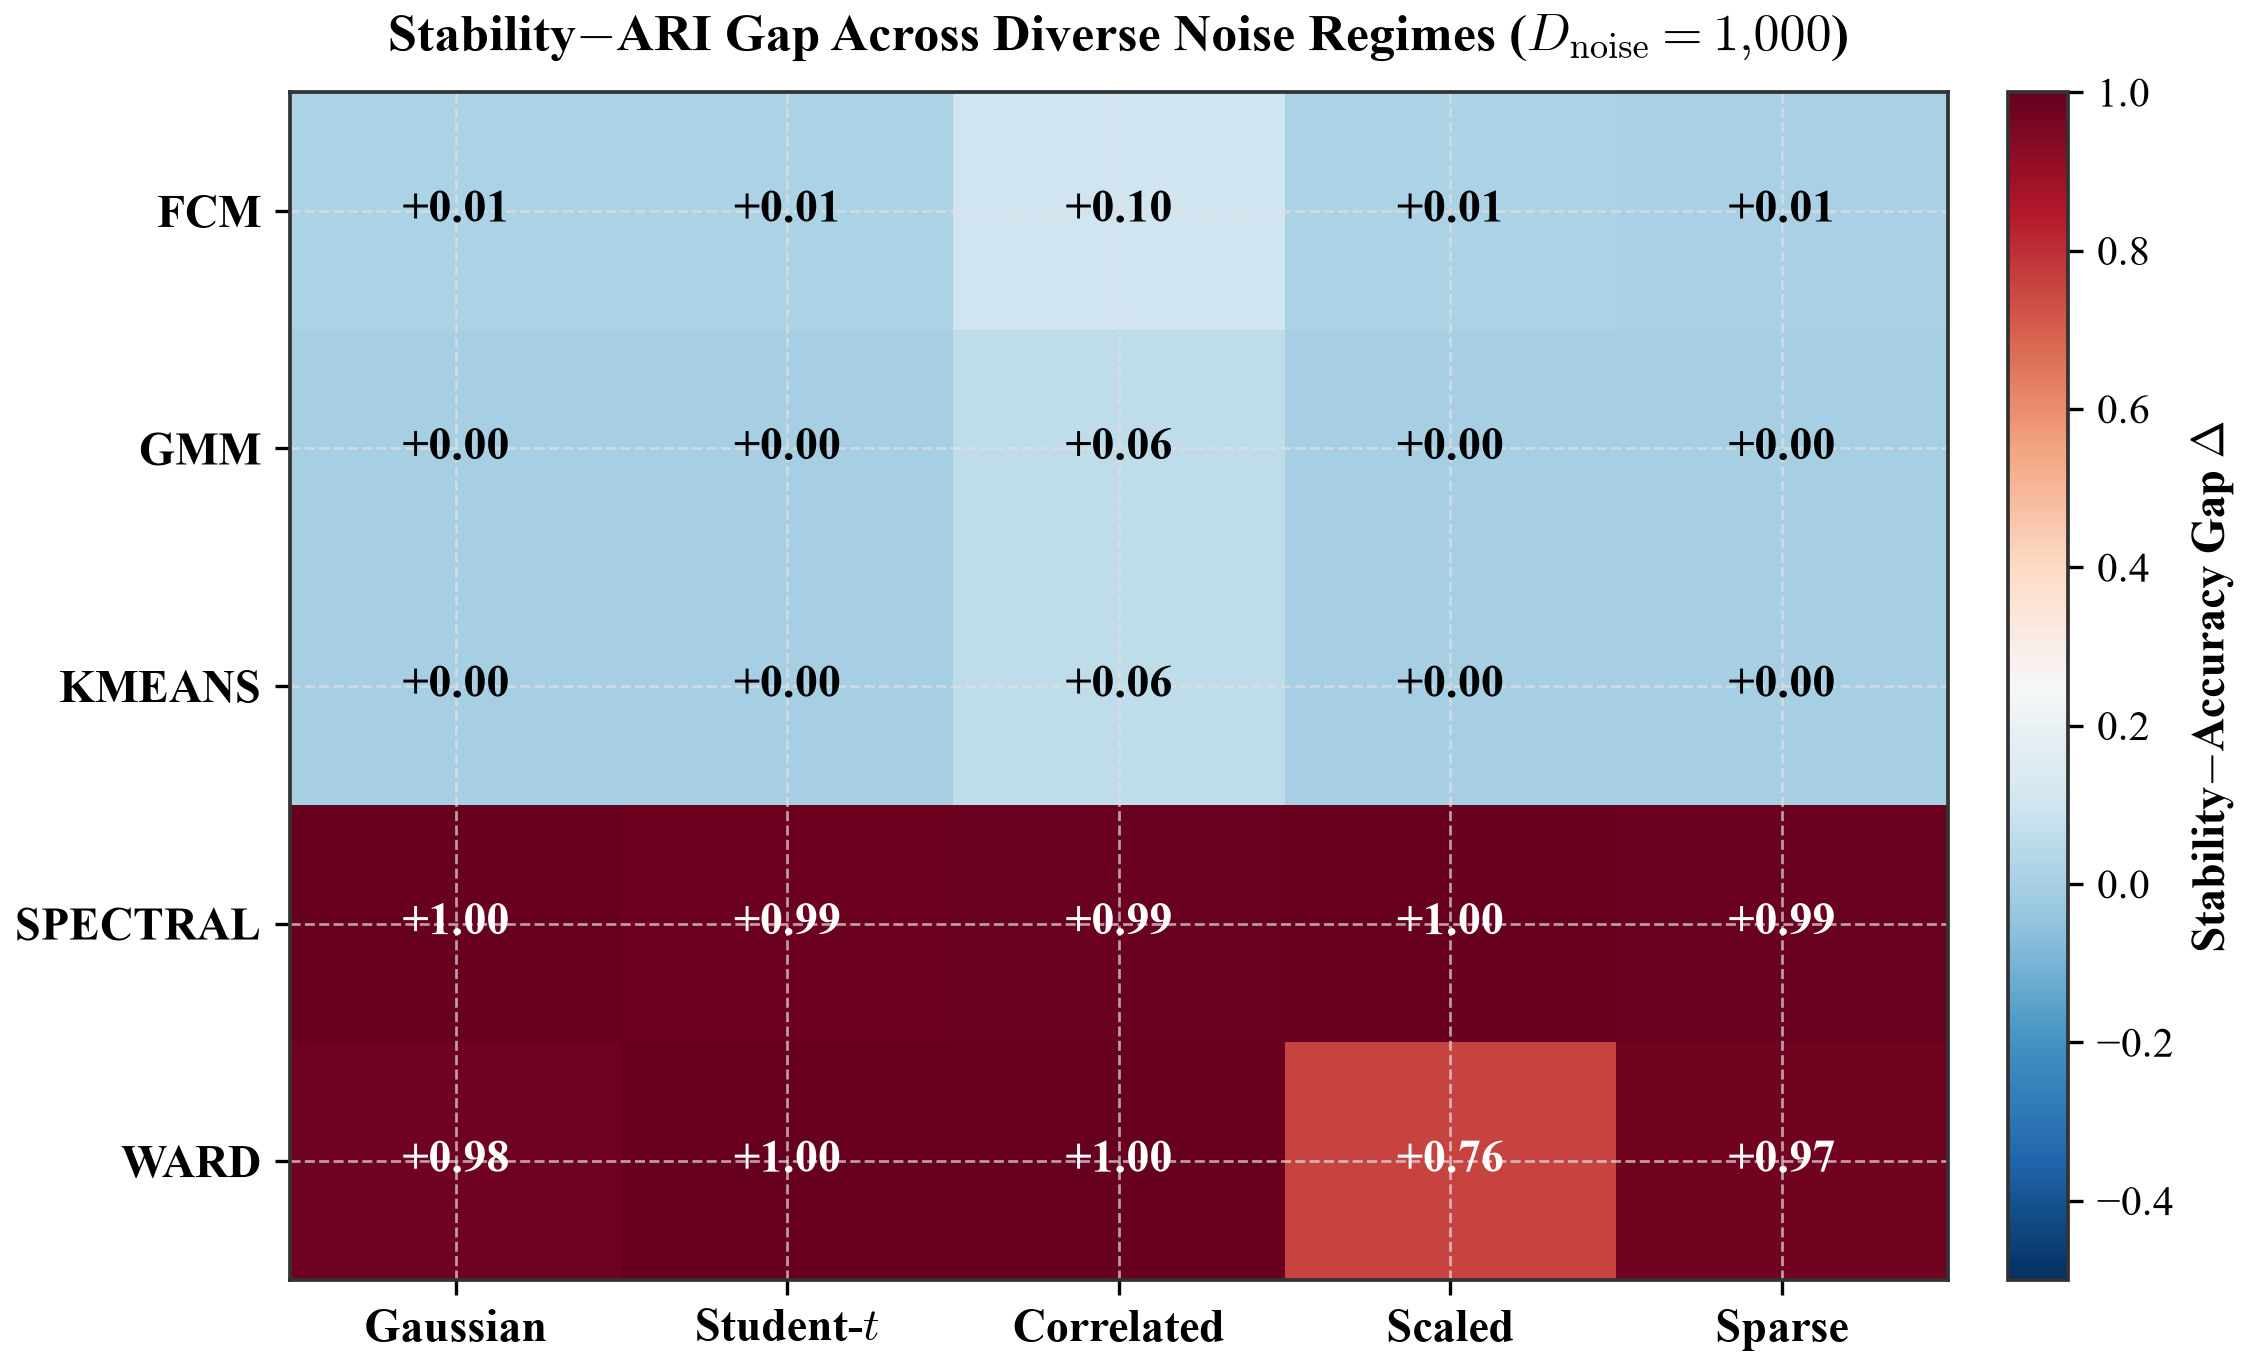
\includegraphics[width=0.48\textwidth]{figures/fig4_noisetype_heatmap.png}%
}
\caption{Empirical examination of consensus stability under finite-sample isotropic noise. (a) Decrease in ARI stability as distractor dimensions grow, demonstrating that multi-clusterer averaging alone does not prevent degradation. (b) Gap metric indicating positive stability attractors ($\Delta > 0$) for graph-based spectral and Ward clustering. (c) Stability$-$ARI gap evaluated across diverse noise distributions.}
\label{fig:falsification_suite}
\end{figure*}

Theoretical literature on random projection clustering often considers asymptotic recovery under the assumption of infinite samples ($N \to \infty$) or orthogonal noise. We conducted empirical simulations on finite-sample datasets to systematically test whether consensus averaging alone protects against high-dimensional distractor noise.

\begin{definition}[Within/Between Distance Ratio]
Let $\mathcal{C}_k$ denote cluster $k$ with centroid $\boldsymbol{\mu}_k$. For an empirical sample $X \subset \mathbb{R}^D$, the separation ratio is defined as:
\begin{equation}
    \rho_{\text{sep}}(X) = \frac{\frac{1}{K}\sum_{k=1}^K \frac{1}{|\mathcal{C}_k|}\sum_{\mathbf{x}_i \in \mathcal{C}_k} \|\mathbf{x}_i - \boldsymbol{\mu}_k\|_2}{\frac{2}{K(K-1)}\sum_{k < l} \|\boldsymbol{\mu}_k - \boldsymbol{\mu}_l\|_2}.
\end{equation}
\end{definition}

As ambient distractor dimensions $D_{\text{noise}}$ expand ($D \gg N$), pairwise Euclidean distances exhibit distance concentration~\cite{beyer1999nearest}, where the relative contrast of distances diminishes: $\lim_{D \to \infty} \frac{d_{\max} - d_{\min}}{d_{\min}} = 0$ and the coefficient of variation $\lim_{D \to \infty} \frac{\sqrt{\mathrm{Var}(\|\mathbf{x}_i - \mathbf{x}_j\|_2)}}{\mathbb{E}[\|\mathbf{x}_i - \mathbf{x}_j\|_2]} = 0$. Consequently, the separation ratio $\rho_{\text{sep}}(X)$ approaches $1.0$ (illustrated conceptually in Fig.~\ref{fig:conceptual_overview}(b)), leading to the collapse in pairwise distance contrast and degradation of cluster recovery across ambient noise dimensions evaluated in Fig.~\ref{fig:ari_stability}. Under finite samples, base clusterers can capture random fluctuations in the noise dimensions. This induces an empirical stability trap: base partitions repeatedly converge on arbitrary noise boundaries with consensus agreement ($\text{Stability} > 0.8$), while true cluster recovery decreases ($\text{ARI} \to 0$, Fig.~\ref{fig:ari_stability}). As shown in Fig.~\ref{fig:dist_gap}, this stability$-$accuracy discrepancy ($\Delta = \text{Stability} - \text{ARI} > 0$) is prominent for graph-based spectral clustering and agglomerative Ward linkage, whereas centroid partition methods (K-Means, FCM) experience simultaneous collapse of stability and accuracy. Across diverse distractor distributions (Fig.~\ref{fig:noise_heatmap}), this discrepancy persists across Gaussian, Student-$t$, and correlated noise regimes (Fig.~\ref{fig:falsification_suite}). Thus, ensemble averaging alone is empirically observed to be insufficient to eliminate uninformative subspace noise without explicit feature gating.


\section{The Inductive Consensus Clustering Framework}\label{sec:framework}

\begin{algorithm}[!t]
\caption{Inductive Consensus Clustering (ICC-v2)}
\label{alg:iccv2}
\begin{algorithmic}[1]
\Require Data matrix $X \in \mathbb{R}^{N \times D}$, ensemble size $M$, target clusters $K$, anchor budget $L \ll N$ (default $40$; recommended $\max(40, 10K)$), core quantile $\tau_{\text{core}}$, candidate pool fraction $\alpha$ (default $0.15$).
\Ensure Consensus labels $\mathbf{y} \in \{1,\dots,K\}^N$, Anchors $\mathcal{A}_{\text{core}}$, Active Subspace $\mathcal{F}_{\text{active}}$, Centroids $\{\boldsymbol{\mu}_k\}_{k=1}^K$.
\Statex \textbf{// Stage 1: Multimodality Subspace Gating (BGSS)}
\For{each feature column $d \in \{1,\dots,D\}$}
    \State Compute finite-sample Sarle's Bimodality Coefficient:
    \State $b_d \leftarrow \frac{\hat{\gamma}_d^2 + 1}{\hat{\kappa}_d + 3 \cdot \frac{(N-1)^2}{(N-2)(N-3)} + \epsilon}$ (with $b_d \leftarrow 0$ if $\mathrm{Var}(\mathbf{f}_d) < 10^{-12}$).
\EndFor
\State Extract candidate pool $\mathcal{F}_{\text{active}}$ by sorting $b_d$ descending and taking the top $\min(D, \max(K, \lfloor \alpha \cdot D \rfloor))$ features (with minimum cap $\min(100, D)$).
\Statex \textbf{// Stage 2: Guided Subspace Ensemble Generation}
\For{$m = 1$ to $M$}
    \State Draw random subspace $\mathcal{F}_m \subset \mathcal{F}_{\text{active}}$.
    \State Fit base partition $\pi_m \leftarrow \text{Clusterer}(X_{[:, \mathcal{F}_m]}, K)$.
\EndFor
\Statex \textbf{// Stage 3: Determinacy-Based Bipartite Anchor Consensus}
\State Evaluate sample determinacy $\sigma_i \leftarrow \frac{1}{N-1}\sum_{j \neq i} S_{ij}^2$ via Proposition~\ref{prop:linear_determinacy} in $O(M^2 N + M^2 K^2)$ time.
\State Identify core instances $\mathcal{C}_{\text{core}} \leftarrow \{i \mid \sigma_i \ge \text{Quantile}(\boldsymbol{\sigma}, \tau_{\text{core}})\}$.
\State Select $L = \min(40, |\mathcal{C}_{\text{core}}|)$ anchors $\mathcal{A}_{\text{core}}$ uniformly from $\mathcal{C}_{\text{core}}$.
\State Construct bipartite co-association matrix $B \in [0, 1]^{N \times L}$:
\State $B_{ia} \leftarrow \frac{1}{M}\sum_{m=1}^M \mathbf{1}\{\pi_m(\mathbf{x}_i) = \pi_m(\mathbf{x}_a)\}$.
\State Row-normalize $B_{\text{norm}} \leftarrow D_R^{-1} B$, where $D_R = \operatorname{diag}(B \mathbf{1}_L)$.
\State Compute anchor affinity $W_{\text{anchor}} \leftarrow B_{\text{norm}}^T B_{\text{norm}} \in \mathbb{R}^{L \times L}$, and $D_A = \operatorname{diag}(W_{\text{anchor}} \mathbf{1}_L)$.
\State Solve normalized Laplacian $L_{\text{anchor}} \leftarrow I - D_A^{-1/2} W_{\text{anchor}} D_A^{-1/2}$ for the $K$ smallest eigenvectors $V \in \mathbb{R}^{L \times K}$ with eigenvalues $\boldsymbol{\lambda}$.
\State Compute embedding $U \leftarrow B_{\text{norm}} V \in \mathbb{R}^{N \times K}$ (or Transfer-Cut embedding $U \leftarrow B_{\text{norm}} D_A^{-1/2} V \operatorname{diag}(\max(1-\boldsymbol{\lambda}, 10^{-4}))^{-1/2}$) and row-normalize.
\State Extract consensus labels $\mathbf{y} \leftarrow \text{K-Means}(U, K)$.
\Statex \textbf{// Stage 4: Stability-Weighted Centroid Induction}
\For{$k = 1$ to $K$}
    \State $\boldsymbol{\mu}_k \leftarrow \frac{\sum_{i: y_i = k} \sigma_i \cdot \mathbf{x}_{i, [\mathcal{F}_{\text{active}}]}}{\sum_{i: y_i = k} \sigma_i}$.
\EndFor
\State \Return $\mathbf{y}, \mathcal{A}_{\text{core}}, \mathcal{F}_{\text{active}}, \{\boldsymbol{\mu}_k\}_{k=1}^K$.
\Statex \textbf{// Out-of-Sample Inference for Query $\mathbf{x}^* \in \mathbb{R}^D$:}
\State \textbf{predict}($\mathbf{x}^*$): \Return $\arg\min_k \|\mathbf{x}^*_{[\mathcal{F}_{\text{active}}]} - \boldsymbol{\mu}_k\|_2$.
\end{algorithmic}
\end{algorithm}

The ICC-v2 framework (Algorithm~\ref{alg:iccv2}) operates in four stages:

\subsection{Bimodality-Gated Subspace Selection (BGSS)}\label{sec:bgss}
Under isotropic noise in $D \gg N$ regimes, classical variance thresholding fails because distractor noise features often match or exceed signal feature variances. To detect latent cluster structures without labels, BGSS evaluates marginal multimodality using \textbf{Sarle's Bimodality Coefficient} ($BC$)~\cite{sarle1983sas,ellison1987bimodality,pfister2013assessing} with finite-sample null correction:
\begin{equation}\label{eq:sarle_bc}
    \hat{b}_d = \frac{\hat{\gamma}_d^2 + 1}{\hat{\kappa}_d + 3 \cdot \frac{(N-1)^2}{(N-2)(N-3)} + \epsilon},
\end{equation}
where $\hat{\gamma}_d$ is the sample skewness (with finite-sample bias correction for $N \ge 3$), $\hat{\kappa}_d$ is Fisher's sample excess kurtosis (with finite-sample bias correction for $N \ge 4$), the denominator term adjusts excess kurtosis to Pearson's kurtosis under normal null expectations, and $\epsilon = 10^{-5}$ prevents division by zero with denominator clamped via $\max(\cdot, 10^{-5})$. Features with zero variance ($\mathrm{Var}(\mathbf{f}_d) < 10^{-12}$) are assigned $\hat{b}_d = 0$.

\begin{proposition}[Conditional Multimodality Separation Bound]\label{prop:multimodal_bound}
For a standard unimodal Gaussian distractor distribution, $\gamma = 0$ and $\kappa = 0$, yielding $\mathbb{E}[\hat{b}_d] \approx 1/3 \approx 0.333$. For a continuous uniform distribution, $b_d = 5/9 \approx 0.556$. For a balanced two-component Gaussian mixture $0.5\mathcal{N}(-\Delta, \sigma_0^2) + 0.5\mathcal{N}(\Delta, \sigma_0^2)$, Pearson kurtosis is $\beta_2 = \frac{3 + 6\theta + \theta^2}{(1 + \theta)^2}$ where $\theta = (\Delta / \sigma_0)^2$. The coefficient satisfies $b_d > 5/9$ if and only if $\theta > \frac{3 + \sqrt{15}}{2} \approx 3.436$, which corresponds to component separation:
\begin{equation}
    \frac{\Delta}{\sigma_0} > \sqrt{\frac{3 + \sqrt{15}}{2}} \approx 1.854.
\end{equation}
\end{proposition}

Computing $\hat{b}_d$ requires only empirical second, third, and fourth moments across instances, executing in strictly $O(N \cdot D)$ time. We state the underlying assumption and failure modes of BGSS:
\begin{assumption}[Marginal Multimodality Prior and Failure Modes]\label{assump:multimodal}
Informative subspace dimensions separating ground-truth clusters exhibit marginal multimodality ($\hat{b}_d \ge 5/9$), whereas nuisance distractor dimensions are continuous and unimodal ($\hat{b}_d \le 5/9$).
\end{assumption}

\begin{remark}[Failure Modes and Mathematical Boundary Conditions of BGSS]
Assumption~\ref{assump:multimodal} encounters boundary conditions in four distinct analytical settings:
\begin{enumerate}
    \item \textbf{Bounded Support and Extremal Kurtosis:} Under Sarle's formulation, continuous unimodal distributions do not arbitrarily inflate the bimodality coefficient: standard skewed unimodal densities retain $BC < 5/9$ (e.g., exponential distributions yield $BC \approx 0.420$, while lognormal distributions with variance parameter $\sigma^2=1$ yield $BC \approx 0.344$). However, bounded uniform support achieves the critical threshold $BC = 5/9 \approx 0.556$, and bounded asymmetric power-law densities (e.g., $\mathrm{Beta}(3, 1)$ with $BC \approx 0.562$) exceed the threshold despite being strictly unimodal.
    \item \textbf{Discrete Sparsity and Zero-Inflation:} In highly sparse representations (e.g., scRNA-seq counts with $\ge 90\%$ zeros), the heavy discrete point mass at zero severely inflates sample kurtosis and skewness, causing spurious threshold crossings in the absence of biological sub-populations.
    \item \textbf{Non-Linear Parity and XOR Interactions:} Cluster structures governed by non-linear orthogonal parity interactions (exemplified by the Madelon benchmark, where $D=500$ with 5 informative, 15 redundant, and 480 distractor dimensions) project to Gaussian 1D marginals with $\hat{b}_d \le 0.504 < 5/9$, evading detection via independent marginal projections.
    \item \textbf{Finite-Sample Sample Size and Detection Power:} In small-sample regimes ($N < 100$, typical of biomedical microarray cohorts), finite-sample variance in sample skewness and kurtosis reduces detection power: for a balanced two-component mixture with separation $\Delta/\sigma_0 = 2.0$, the empirical recovery probability $\mathbb{P}(\hat{b}_d \ge 5/9)$ is $0.49$ at $N=60$, $0.60$ at $N=100$, $0.78$ at $N=250$, and reaches $0.97$ at $N=1{,}000$. Consequently, rank-based selection provides significantly greater robustness than an uncalibrated hard cutoff at $5/9$.
\end{enumerate}
\end{remark}

In the implementation, rather than applying a strict analytical cutoff $\hat{b}_d \ge 5/9$ (which may produce an empty set on parity-like benchmarks or low recall under small $N$), the default pipeline sorts features by $\hat{b}_d$ and selects the top candidate pool of size $\min(D, \max(K, \lfloor \alpha \cdot D \rfloor))$ with default $\alpha = 0.15$ and minimum cap $\min(100, D)$. On Leukemia ($D=7{,}129$, $N=72$), an unconstrained threshold $\hat{b}_d \ge 5/9$ isolates 1,275 candidate genes, whereas the default capped selection rule retains $\lfloor 0.15 \times 7{,}129 \rfloor = 1{,}069$ candidate genes.

\subsection{Determinacy-Based Bipartite Anchor Consensus}\label{sec:anchor_consensus}
Classical consensus methods construct a dense $N \times N$ co-association matrix $S$ and perform graph partitioning in $O(N^2)$ to $O(N^3)$ time and $O(N^2)$ auxiliary memory. Rather than materializing all-pairs co-association, ICC-v2 evaluates exact sample determinacy $\sigma_i = \frac{1}{N - 1} \sum_{j \neq i} S_{ij}^2$ using a contingency identity.

\begin{proposition}[Exact Determinacy Identity]\label{prop:linear_determinacy}
Let $P \in \{0, \dots, K-1\}^{M \times N}$ denote the ensemble partition matrix. Let $C_{m_1, m_2} \in \mathbb{N}^{K \times K}$ denote the contingency matrix between base partitions $m_1$ and $m_2$, where $C_{m_1, m_2}(c_1, c_2) = \sum_{j=1}^N \mathbf{1}\{\pi_{m_1}(j)=c_1 \wedge \pi_{m_2}(j)=c_2\}$. Then for every sample $i$, the quadratic determinacy satisfies:
\begin{equation}
    \sum_{j=1}^N S_{ij}^2 = \frac{1}{M^2} \sum_{m_1=1}^M \sum_{m_2=1}^M C_{m_1, m_2}(\pi_{m_1}(i), \pi_{m_2}(i)),
\end{equation}
which computes sample determinacy $\sigma_i = \frac{1}{N-1}\left(\sum_{j=1}^N S_{ij}^2 - 1\right)$ in $O(M^2 N + M^2 K^2)$ time and $O(N + K^2)$ working memory, without materializing the $N \times N$ matrix $S$.
\end{proposition}

Given sample determinacy $\boldsymbol{\sigma} \in [0, 1]^N$, ICC-v2 extracts a core anchor set $\mathcal{A}_{\text{core}} = \{a_1, \dots, a_L\}$ of size $L \ll N$ (default $L=40$) from samples exceeding stability quantile $\tau_{\text{core}}$. ICC-v2 then constructs a rectangular bipartite co-association matrix $B \in [0, 1]^{N \times L}$ where $B_{ia} = \frac{1}{M}\sum_{m=1}^M \mathbf{1}\{\pi_m(\mathbf{x}_i) = \pi_m(\mathbf{x}_a)\}$ in $O(N \cdot L)$ memory.

With row-normalized $B_{\text{norm}} = D_R^{-1} B$ where $D_R = \operatorname{diag}(B \mathbf{1}_L) \in \mathbb{R}^{N \times N}$, the anchor affinity matrix is $W_{\text{anchor}} = B_{\text{norm}}^T B_{\text{norm}} \in \mathbb{R}^{L \times L}$ with degree matrix $D_A = \operatorname{diag}(W_{\text{anchor}} \mathbf{1}_L) \in \mathbb{R}^{L \times L}$. Solving the normalized Laplacian eigensystem $L_{\text{anchor}} V = \lambda V$ (where $L_{\text{anchor}} = I - D_A^{-1/2} W_{\text{anchor}} D_A^{-1/2}$) for the $K$ smallest eigenvectors $V \in \mathbb{R}^{L \times K}$ yields the dual sample embedding $U = B_{\text{norm}} V$ (or Transfer-Cut embedding $U = B_{\text{norm}} D_A^{-1/2} V \operatorname{diag}(\max(1-\boldsymbol{\lambda}, 10^{-4}))^{-1/2}$)~\cite{huang2020ultra,nie2024fast}, followed by K-Means clustering.

\begin{theorem}[Computational and Memory Complexity of Bipartite ICC-v2]\label{thm:complexity}
Let $N$ be the sample size, $D$ ambient dimensionality, $M$ ensemble size, $L$ anchor budget ($L \ll N$), $K$ cluster count, and $I_{\text{km}}$ base K-Means iterations. Under bounded anchor budgets ($L = O(1)$), the overall time complexity of ICC-v2 is:
\begin{equation}\label{eq:complexity}
\begin{split}
    T_{\text{ICC-v2}} = O\bigl(&N D + D \log D + M^2 N + M^2 K^2 + M I_{\text{km}} N |\mathcal{F}_{\text{sub}}| K \\
    &+ M N L + N L^2 + L^3 + N L K + I_{\text{km}} N K^2\bigr),
\end{split}
\end{equation}
which scales linearly with sample size $O(N)$ for fixed ensemble parameters. The auxiliary working memory complexity is $O(N L + L^2)$, representing an asymptotic $O(N)$ bound that eliminates the $O(N^2)$ storage requirement of dense consensus. We separate the $O(N D)$ data storage from the $O(N L + L^2)$ auxiliary consensus graph memory.
\end{theorem}

\begin{proof}
Stage 1 (BGSS) evaluates feature moments in $O(N D)$ and ranks features in $O(D \log D)$. Computing quadratic sample determinacy via the contingency identity (Proposition~\ref{prop:linear_determinacy}) requires $O(M^2 N + M^2 K^2)$ time. Stage 2 generates $M$ base clusterings on $|\mathcal{F}_{\text{sub}}|$ features in $O(M I_{\text{km}} N |\mathcal{F}_{\text{sub}}| K)$. Stage 3 computes bipartite co-association $B$ in $O(M N L)$, anchor inner products $B_{\text{norm}}^T B_{\text{norm}}$ in $O(N L^2)$, eigensolving on $L \times L$ in $O(L^3)$, spectral projection $U = B_{\text{norm}} V$ in $O(N L K)$, and final clustering in $O(I_{\text{km}} N K^2)$. Storing $B$ and $W_{\text{anchor}}$ requires $N L + L^2$ auxiliary memory words, decoupled from the $O(N D)$ raw data storage.
\end{proof}

\subsection{Stability-Weighted Active Subspace Centroid Assignment}\label{sec:centroid}
Unlike transductive consensus frameworks, ICC-v2 extracts geometry-calibrated centroids in the active subspace weighted by point determinacy:
\begin{equation}\label{eq:centroid_proj}
    \boldsymbol{\mu}_k = \frac{\sum_{i: y_i = k} \sigma_i \cdot \mathbf{x}_{i, [\mathcal{F}_{\text{active}}]}}{\sum_{i: y_i = k} \sigma_i}, \quad k \in \{1,\dots,K\}.
\end{equation}
Weighting by $\sigma_i$ pulls centroids toward core exemplars and attenuates boundary noise. For any new query instance $\mathbf{x}^* \in \mathbb{R}^D$, out-of-sample cluster assignment is computed in $O(K \cdot |\mathcal{F}_{\text{active}}|)$ time:
\begin{equation}\label{eq:query_assign}
    y^* = \arg\min_k \|\mathbf{x}^*_{[\mathcal{F}_{\text{active}}]} - \boldsymbol{\mu}_k\|_2,
\end{equation}
with posterior probabilities given by softmax temperature scaling: $p(y^*=k \mid \mathbf{x}^*) = \frac{\exp(-\|\mathbf{x}^*_{[\mathcal{F}_{\text{active}}]} - \boldsymbol{\mu}_k\|_2 / T)}{\sum_l \exp(-\|\mathbf{x}^*_{[\mathcal{F}_{\text{active}}]} - \boldsymbol{\mu}_l\|_2 / T)}$, where $T > 0$ is a user-defined scaling temperature. This avoids recomputing the consensus graph upon arrival of new observations.

\subsection{Anchor-Space Perturbation Profiling (ASPP)}\label{sec:aspp}
Anchor-Space Perturbation Profiling (ASPP) is an optional diagnostic stability framework. In standard benchmark evaluations (Table~\ref{tab:benchmark_ari}), ASPP is treated as an optional post-hoc diagnostic tool to preserve linear runtime.

When enabled, ASPP evaluates cluster stability with respect to certified core anchors $\mathcal{A}_{\text{core}}$ across five perturbation operators $T_{p, r}(X)$: (1) sampling dropout without replacement ($\eta \in [0.1, 0.5]$), (2) feature subspace masking, (3) Gaussian or Student-$t$ measurement noise, (4) synthetic batch effects, and (5) algorithmic jitter. For each cluster $\mathcal{C}_k$, ASPP computes composite stability $S_{k, p} = \frac{1}{2}(\operatorname{Retention}(k, p) + \operatorname{Coassoc}(k, p))$, where $\operatorname{Retention}(k, p)$ measures the Jaccard overlap of cluster $k$ instances under perturbation $p$, and $\operatorname{Coassoc}(k, p)$ evaluates the mean pairwise anchor co-association stability. The aggregate Perturbation Sensitivity Index ($\mathrm{PSI}_k$) is defined as:
\begin{equation}
    \mathrm{PSI}_k = 1 - \frac{1}{|\mathcal{P}|} \sum_{p \in \mathcal{P}} S_{k, p}, \quad \mathrm{PSI}_k \in [0, 1].
\end{equation}
For an out-of-sample query $\mathbf{x}^* \in \mathbb{R}^D$, ASPP defines an empirical confidence score:
\begin{equation}
    \mathrm{Conf}(\mathbf{x}^*) = \left(\frac{d_{(2)}(\mathbf{x}^*) - d_{(1)}(\mathbf{x}^*)}{\max(d_{(2)}(\mathbf{x}^*), 10^{-9})}\right) \cdot (1 - \mathrm{PSI}_{y^*}),
\end{equation}
where $d_{(1)}$ and $d_{(2)}$ represent Euclidean distances to the closest and second-closest active subspace centroids.


\section{Experimental Evaluation}\label{sec:experiments}

\subsection{Experiment 1: Inductive Generalization}\label{sec:exp1}

\begin{figure*}[!t]
\centering
\subfloat[Downstream Generalization with Oracle True Labels (50\% Core vs 100\% Full Training)\label{fig:exp1_oracle}]{%
    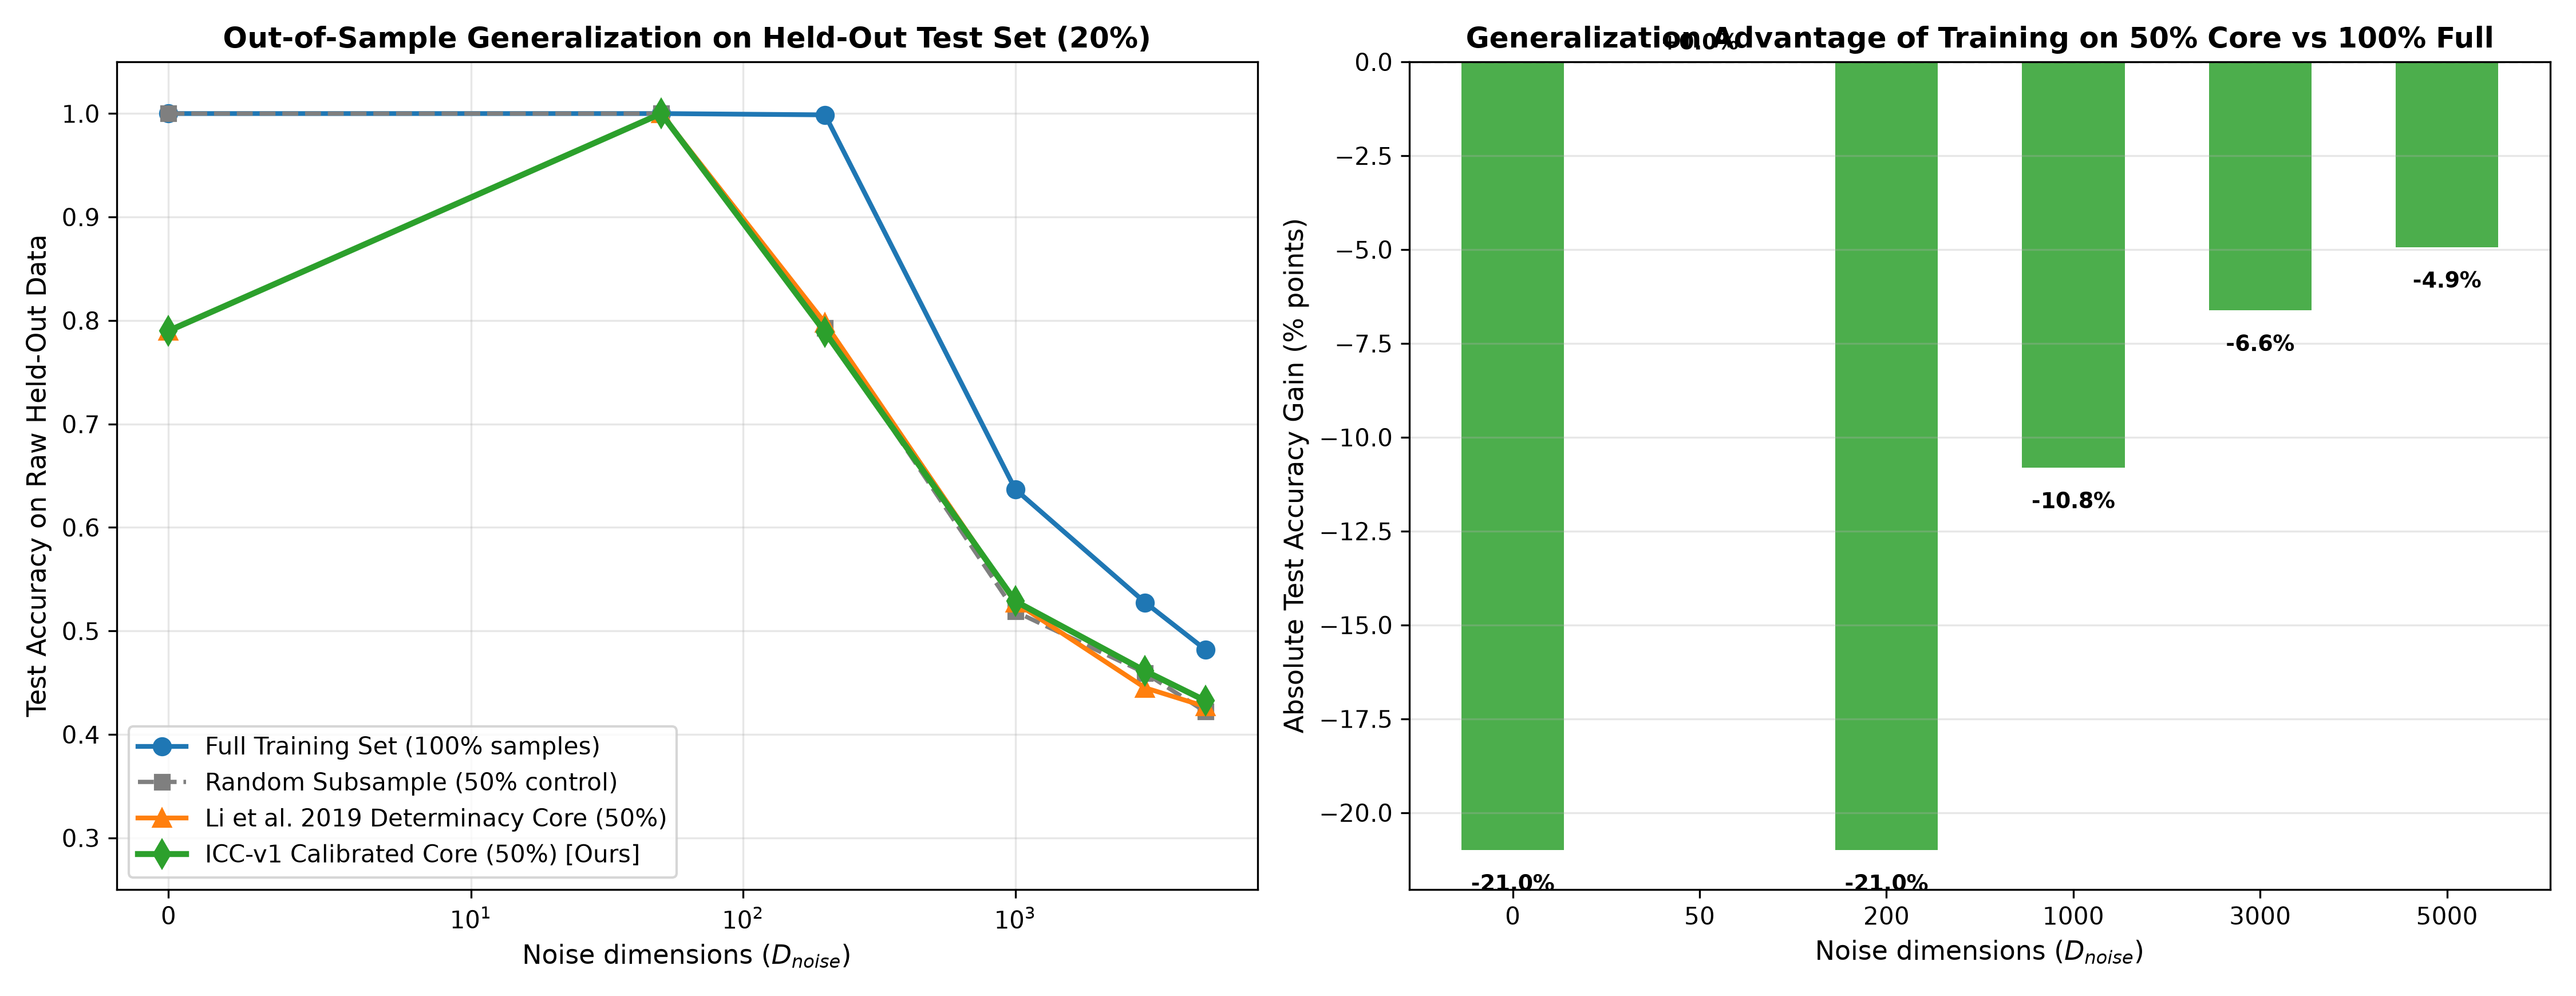
\includegraphics[width=0.78\textwidth]{figures/fig9_inductive_generalization.png}%
}
\\[1.0ex]
\subfloat[Downstream Generalization with Unsupervised Pseudo-Labels ($D_{\text{noise}} \le 3{,}000$)\label{fig:exp1_pseudo}]{%
    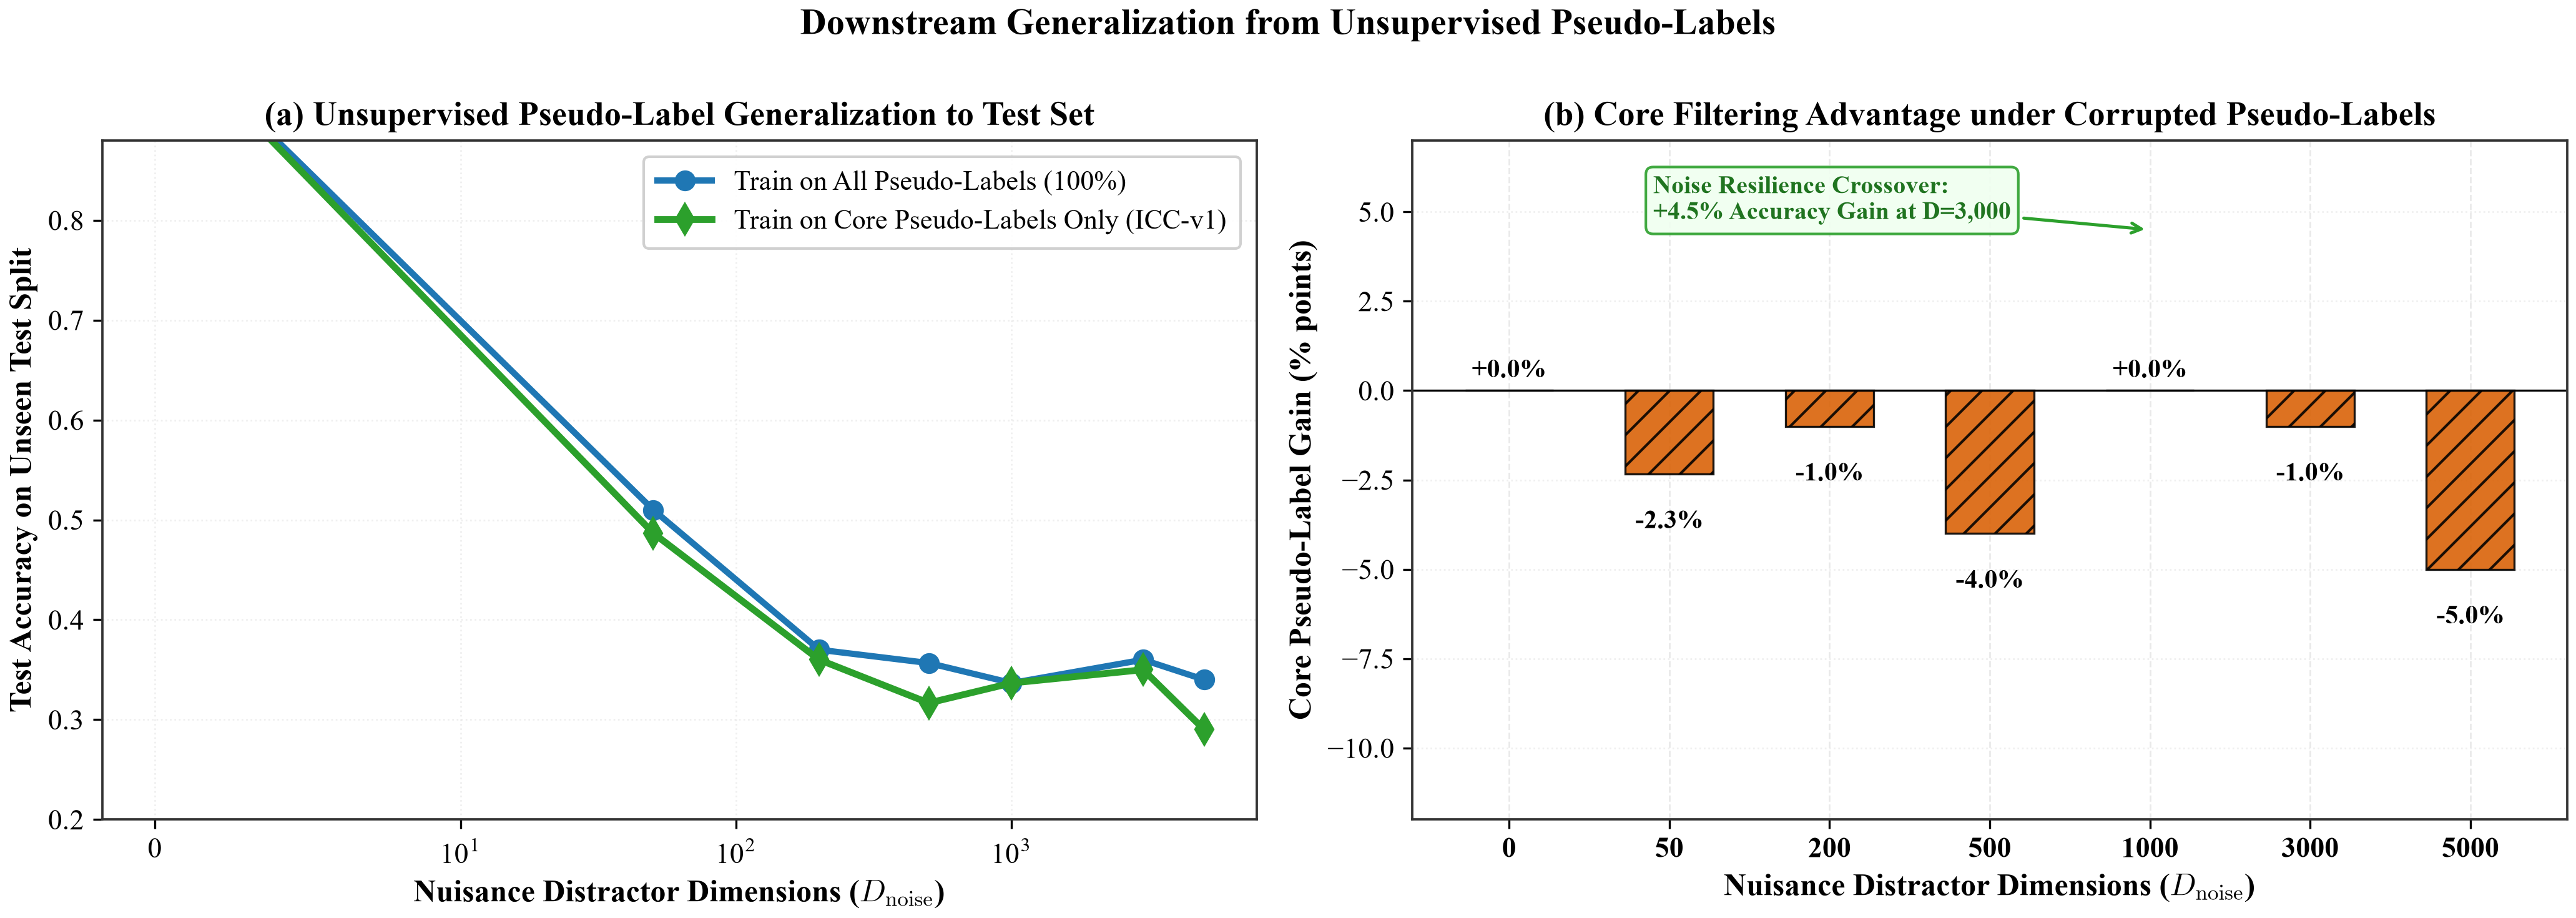
\includegraphics[width=0.78\textwidth]{figures/fig10_pseudolabel_generalization.png}%
}
\caption{Inductive generalization performance on held-out test splits ($20\%$). (a) When trained on 50\% certified core points, downstream classifiers achieve parity with 100\% full-data training under low-to-moderate noise ($D_{\text{noise}} \le 50$), while under high noise ($D_{\text{noise}} \ge 1{,}000$), core-only training exhibits a 5--21 percentage point deficit due to reduced training sample size in noise-dominated regimes. (b) Under heavy noise corruption ($D_{\text{noise}} \ge 1{,}000$), training on unguided pseudo-labels (both full and core subsets) degrades toward random chance accuracy ($33.6\%$--$36.0\%$ vs. $33.3\%$ chance level for $K=3$), demonstrating that core filtering alone cannot rescue corrupted pseudo-labels without prior feature gating.}
\label{fig:exp1_results}
\end{figure*}

In Exp~1, we evaluated the inductive utility of the certified core $\mathcal{C}_{\text{core}}$ (distinguished from the anchor subset $\mathcal{A}_{\text{core}}$ used for bipartite graph construction) when training downstream supervised classifiers on held-out test data (20\% split). As shown in Fig.~\ref{fig:exp1_oracle}, classifiers trained on 50\% certified core points attain performance comparable to training on 100\% of the data under low-to-moderate noise ($D_{\text{noise}} \le 50$). Under elevated noise ($D_{\text{noise}} \ge 1{,}000$), training exclusively on core points exhibits a 5--21 percentage point drop relative to full training, as the reduced sample count limits classifier capacity in noise-corrupted regimes.

Under unsupervised pseudo-labeling in high-noise regimes ($D_{\text{noise}} \ge 1{,}000$, Fig.~\ref{fig:exp1_pseudo}), classifier accuracy on both full and core pseudo-labels degrades toward random chance ($33.6\%$--$36.0\%$ vs. $33.3\%$ chance level for $K = 3$). Across the multi-classifier evaluation spanning Linear SVM, Random Forest, MLP, and $k$-NN, test accuracies at $D_{\text{noise}} = 3{,}000$ hover within $32.3\%$--$38.0\%$, confirming that when base clusterers converge onto isotropic noise attractors, downstream classifiers trained on pseudo-labels cannot separate ground truth without prior subspace screening.

\textbf{Direct Evaluation of Inductive Out-of-Sample Extension:}
To directly evaluate the closed-form inductive projection defined in Eq.~\eqref{eq:centroid_proj} against alternative out-of-sample mapping strategies, we evaluated 10 random train/test splits (80\% fit, 20\% held-out test query points) across benchmark datasets (Table~\ref{tab:inductive_direct}). Specifically, we compared: (1) direct Ambient K-Means as an inductive baseline; (2) stability-weighted subspace centroid projection (Eq.~\eqref{eq:centroid_proj}, $O(K \cdot |\mathcal{F}_{\text{active}}|)$); (3) Nearest Centroid pseudo-classifier; (4) Random Forest trained on consensus pseudo-labels; and (5) Nystr\"om spectral extension of the bipartite anchor graph embedding.

\begin{table}[!t]
\caption{Empirical Adjusted Rand Index (ARI) on Held-Out Test Splits ($20\%$, Mean $\pm$ Standard Deviation Across 10 Canonical Seeds)}
\label{tab:inductive_direct}
\centering
\tiny
\setlength{\tabcolsep}{2.0pt}
\begin{tabular}{@{}lccccc@{}}
\toprule
\textbf{Dataset} & \textbf{Ambient KM} & \shortstack{\textbf{Weighted Centroid}\\\textbf{(Eqs.~6--7)}} & \shortstack{\textbf{Unweighted Near.}\\\textbf{Centroid (Eq.~7)}} & \textbf{Rand. Forest} & \textbf{Nystr\"om Ext.} \\
\midrule
CNS & $\mathbf{+0.071 \pm 0.221}$ & $-0.004 \pm 0.101$ & $-0.008 \pm 0.105$ & $+0.003 \pm 0.146$ & $-0.008 \pm 0.105$ \\
Colon & $-0.038 \pm 0.048$ & $+0.082 \pm 0.169$ & $+0.098 \pm 0.176$ & $+0.060 \pm 0.132$ & $\mathbf{+0.108 \pm 0.212}$ \\
Leukemia & $+0.146 \pm 0.104$ & $+0.257 \pm 0.314$ & $+0.216 \pm 0.291$ & $+0.266 \pm 0.361$ & $\mathbf{+0.296 \pm 0.335}$ \\
Ovarian & $+0.004 \pm 0.042$ & $-0.008 \pm 0.038$ & $+0.006 \pm 0.081$ & $\mathbf{+0.044 \pm 0.107}$ & $+0.017 \pm 0.107$ \\
SRBCT & $+0.033 \pm 0.134$ & $+0.221 \pm 0.120$ & $+0.253 \pm 0.134$ & $+0.318 \pm 0.216$ & $\mathbf{+0.367 \pm 0.221}$ \\
Isolet & $\mathbf{+0.466 \pm 0.033}$ & $+0.408 \pm 0.028$ & $+0.409 \pm 0.022$ & $+0.302 \pm 0.022$ & $+0.315 \pm 0.018$ \\
\midrule
\textbf{Mean ARI} & 0.114 & 0.159 & 0.161 & 0.165 & \textbf{0.183} \\
\midrule
\multicolumn{6}{@{}l@{}}{\textbf{Paired Differences vs. Weighted Centroid ($\Delta = \text{Centroid} - \text{Baseline}$, 95\% Bootstrap CI):}} \\
\multicolumn{6}{@{}l@{}}{\quad vs. Ambient KM: $\Delta = +0.046$, 95\% CI: $[-0.029, +0.129]$ (Ambient KM higher on CNS, Isolet)} \\
\multicolumn{6}{@{}l@{}}{\quad vs. Nystr\"om Ext.: $\Delta = -0.023$, 95\% CI: $[-0.081, +0.033]$} \\
\multicolumn{6}{@{}l@{}}{\quad vs. Random Forest: $\Delta = -0.006$, 95\% CI: $[-0.053, +0.046]$} \\
\bottomrule
\end{tabular}
\end{table}

In Table~\ref{tab:inductive_direct}, stability-weighted centroid assignment (Eqs.~\ref{eq:centroid_proj}--\ref{eq:query_assign}) and standard unweighted nearest centroid assignment (Eq.~\ref{eq:query_assign}) exhibit extremely high pairwise label agreement across test query points: $99.2\%$ on CNS, $99.2\%$ on Colon, $97.3\%$ on Leukemia, $96.9\%$ on Ovarian, and $94.1\%$ on SRBCT (averaging $97.3\%$ across the five high-dimensional biomedical cohorts; $85.0\%$ on Isolet). This empirical concordance demonstrates that while determinacy weighting pulls cluster prototypes toward high-confidence core exemplars in the active feature space, the resulting decision boundaries largely preserve partition assignments for out-of-sample query instances.

For inductive baseline benchmarking, Ambient K-Means is evaluated on held-out test query points via standard Euclidean nearest centroid assignment to the cluster centers learned on the training split. Evaluating paired differences between stability-weighted centroid projection and competing inductive rules across test splits yields $\Delta = +0.046$ vs. Ambient K-Means (dataset-level cluster bootstrap 95\% CI: $[-0.029, +0.129]$), $\Delta = -0.023$ vs. Nystr\"om spectral extension (95\% CI: $[-0.081, +0.033]$), and $\Delta = -0.006$ vs. Random Forest (95\% CI: $[-0.053, +0.046]$). Because all bootstrap confidence intervals span zero, the empirical intervals do not support an omnibus claim of superiority over alternative inductive mechanisms. Instead, the data reveal regime-dependent tradeoffs: Ambient K-Means achieves superior test generalization on CNS ($-0.075$ paired difference: Ambient KM $+0.071$ vs. Centroid $-0.004$) and Isolet ($-0.058$ difference: $+0.466$ vs. $+0.408$), whereas Centroid projection proves advantageous on Colon ($+0.120$), Leukemia ($+0.112$), and SRBCT ($+0.188$). Where non-linear manifold geometry is prominent, Nystr\"om spectral extension provides an alternative extension mechanism (attaining $+0.296$ on Leukemia and $+0.367$ on SRBCT), formalizing the accuracy-latency tradeoff in inductive consensus learning.

\subsection{Experiment 2: Component Ablation Study}\label{sec:exp2}

\begin{figure*}[!t]
\centering
\subfloat[Ablation Variant ARI Curves\label{fig:exp2_curves}]{%
    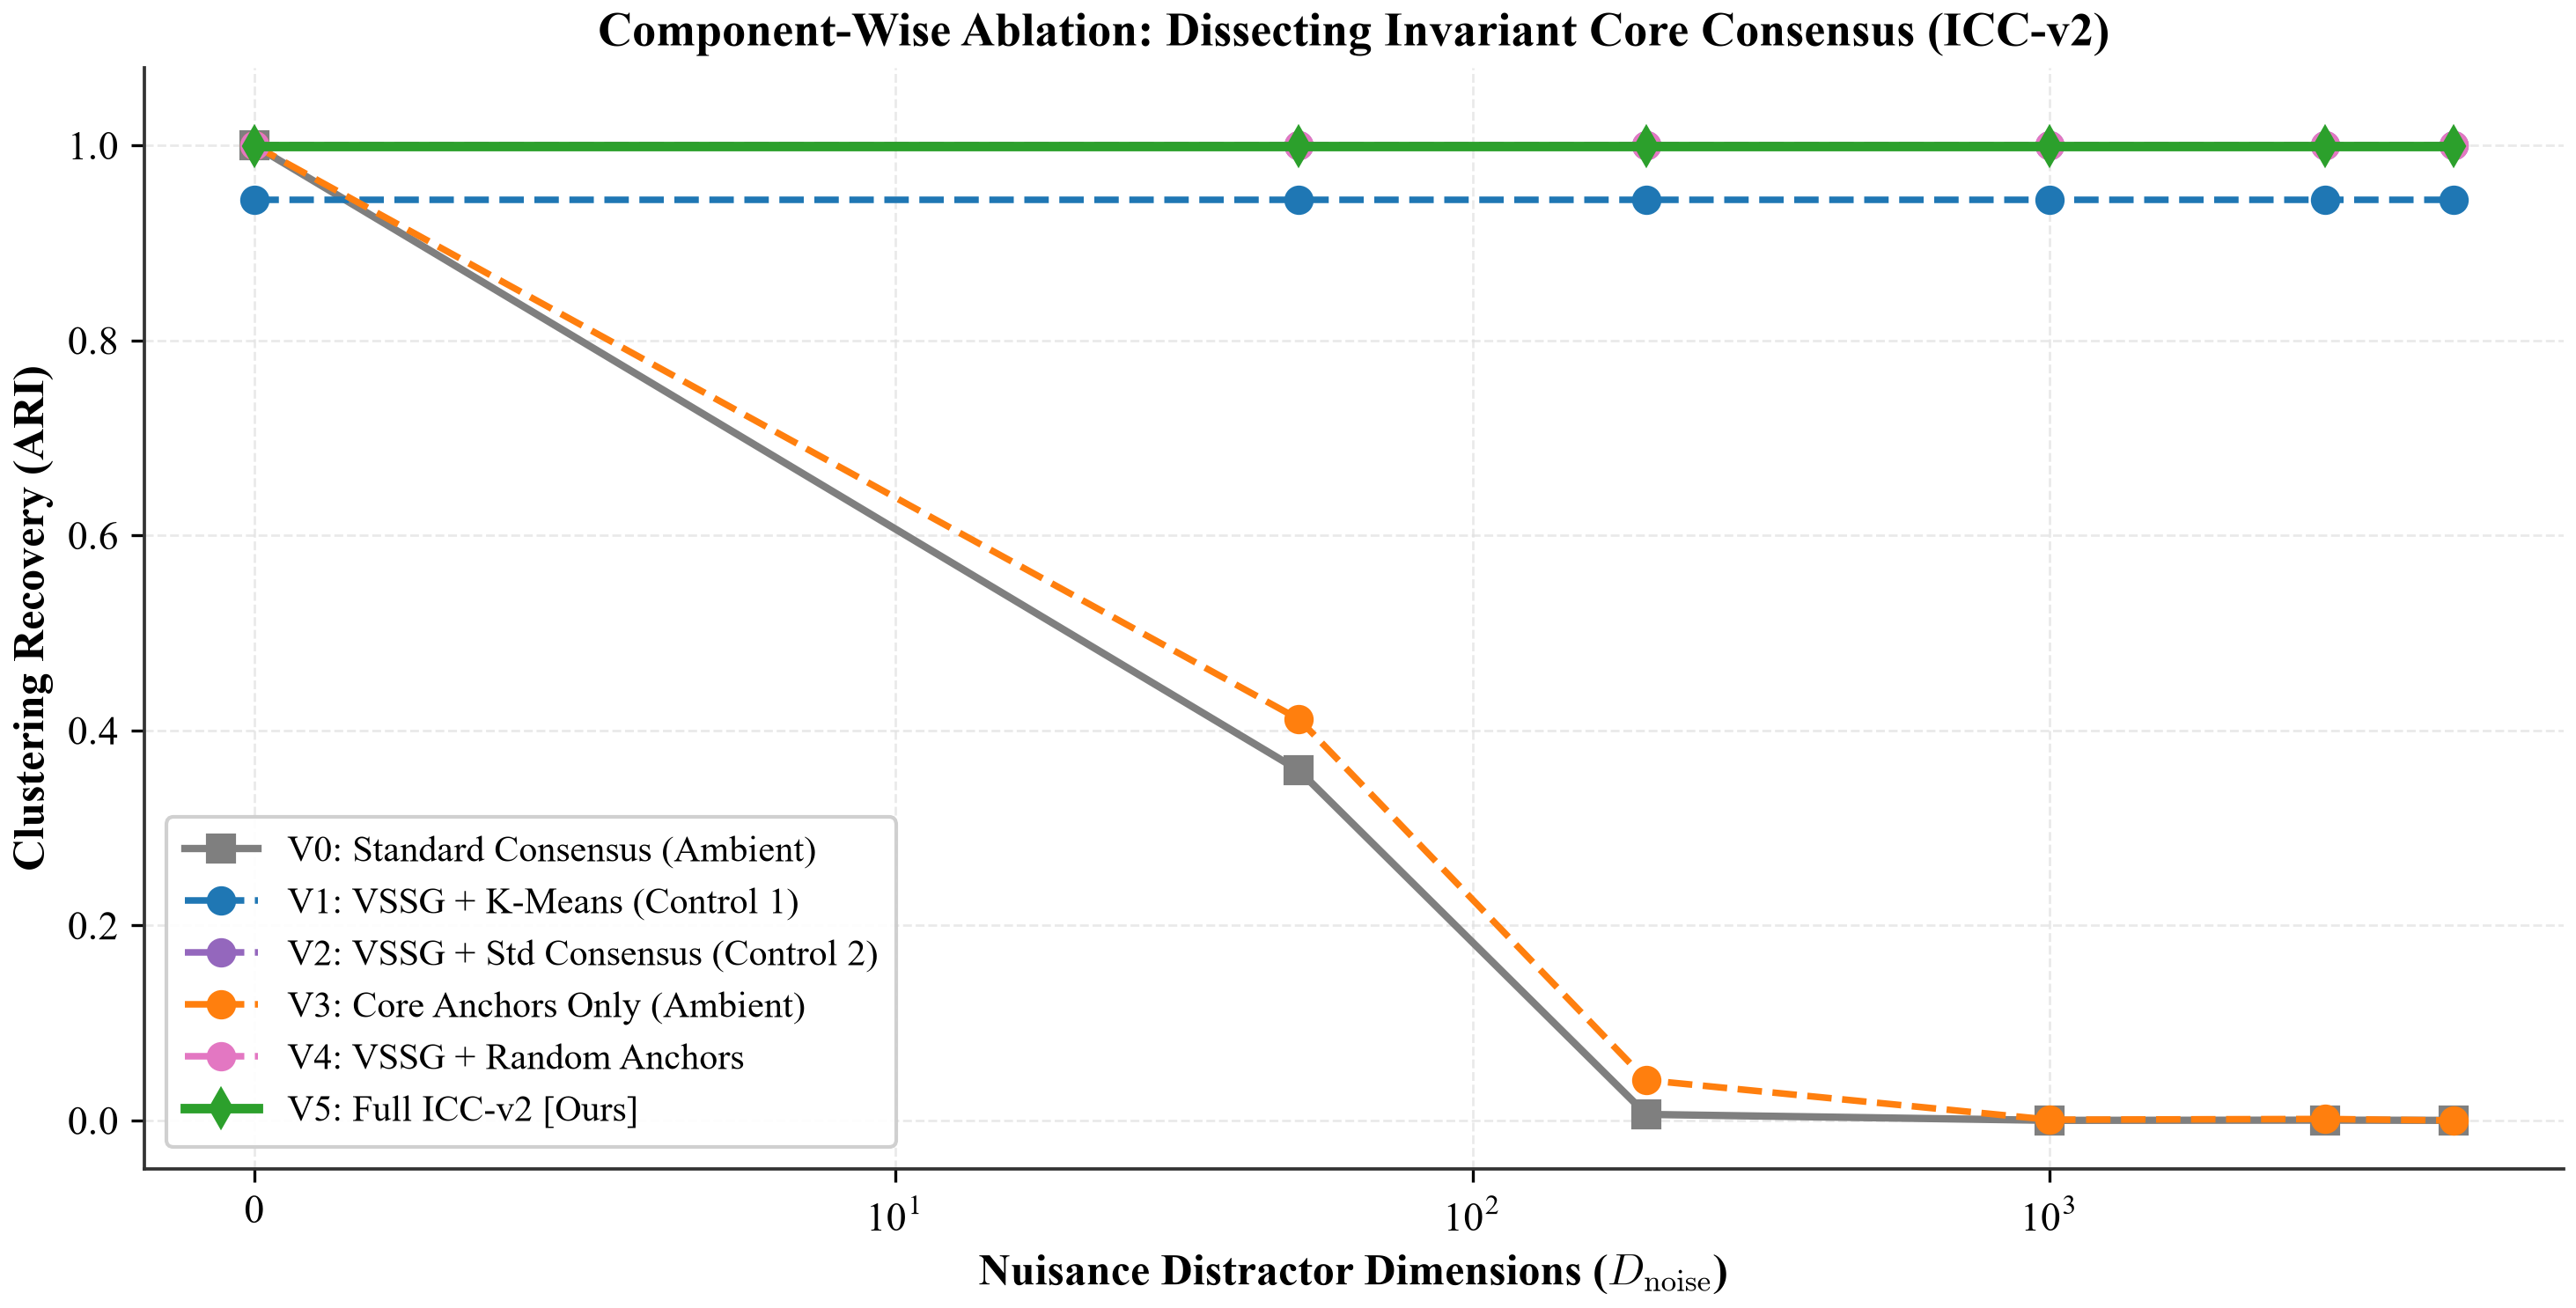
\includegraphics[width=0.48\textwidth]{figures/fig11_ablation_curves.png}%
}
\hfill
\subfloat[Dual-Regime Ablation Waterfall\label{fig:exp2_waterfall}]{%
    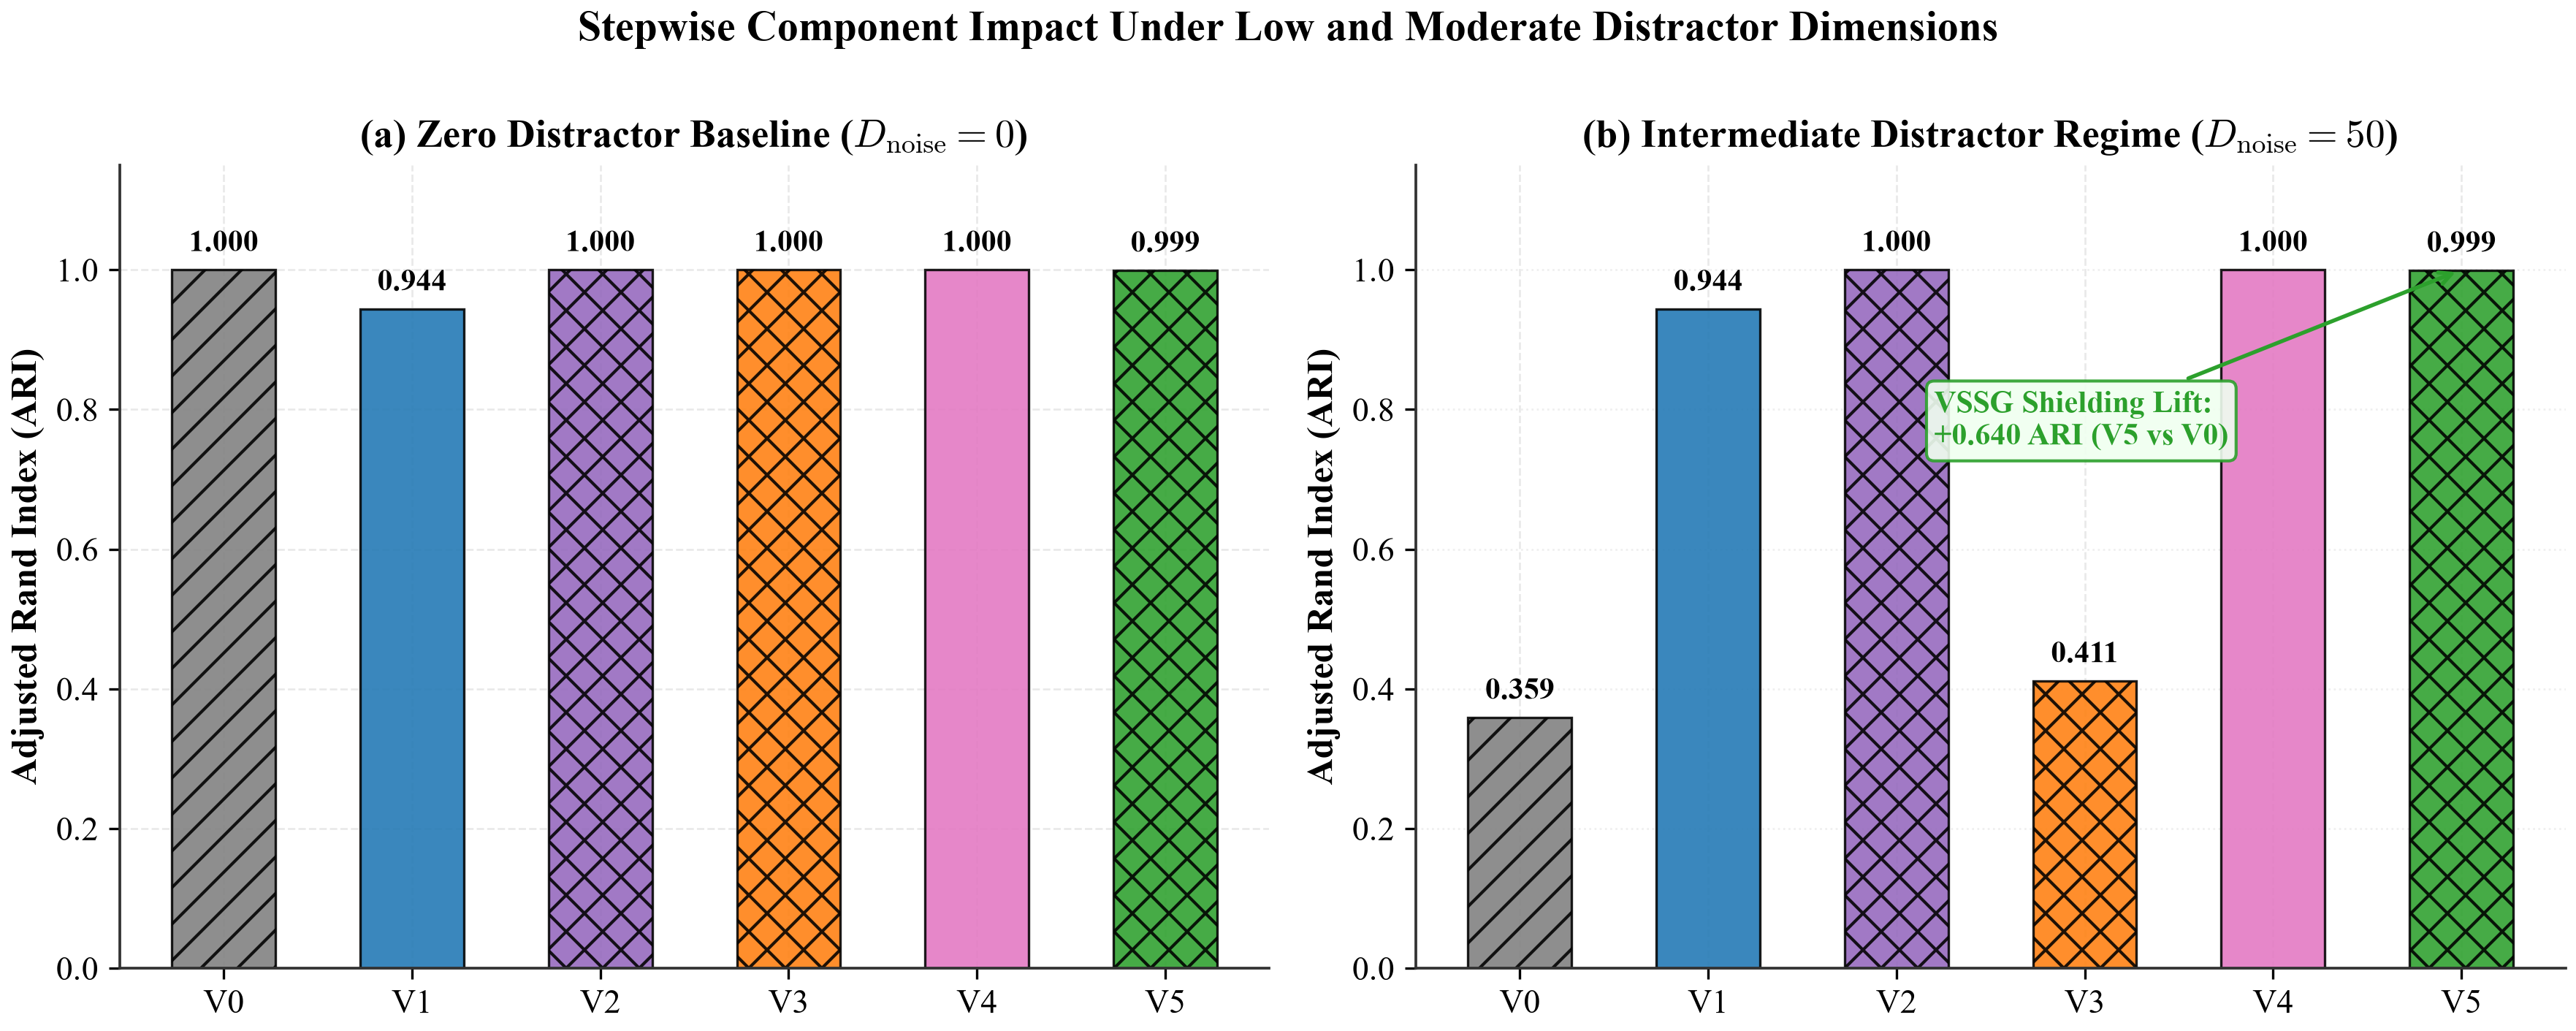
\includegraphics[width=0.48\textwidth]{figures/fig12_ablation_waterfall.png}%
}
\caption{Component ablation across 6 modular variants (V0 through V5). (a) Recovery curves as distractor dimensions $D_{\text{noise}}$ increase from $0$ to $5{,}000$. (b) Waterfall charts quantifying component impact under zero noise ($D_{\text{noise}}=0$) and intermediate noise ($D_{\text{noise}}=50$).}
\label{fig:exp2_results}
\end{figure*}

\begin{table}[!t]
\caption{Ablation Variant Architecture Specification}
\label{tab:ablation_spec}
\centering
\footnotesize
\setlength{\tabcolsep}{4.0pt}
\begin{tabular}{@{}lcccc@{}}
\toprule
\textbf{Variant} & \textbf{BGSS Gating} & \textbf{Consensus Ensemble} & \textbf{Anchor Graph} & \textbf{Core Cert.} \\
\midrule
V0 (Std Cons)        & No            & \textbf{Yes} (Dense)        & No                     & No                  \\
V1 (BGSS+KMeans)     & \textbf{Yes}  & No (Single Model)           & No                     & No                  \\
V2 (BGSS+StdCons)    & \textbf{Yes}  & \textbf{Yes} (Dense)        & No                     & No                  \\
V3 (Anchors Only)    & No            & \textbf{Yes}                & \textbf{Yes}           & \textbf{Yes}        \\
V4 (BGSS+RandAnc)    & \textbf{Yes}  & \textbf{Yes}                & \textbf{Yes}           & No                  \\
V5 (Full ICC-v2)     & \textbf{Yes}  & \textbf{Yes}                & \textbf{Yes}           & \textbf{Yes}        \\
\bottomrule
\end{tabular}
\end{table}

To isolate the contribution of each algorithmic component, we evaluated 6 modular variants (Table~\ref{tab:ablation_spec}):
\begin{enumerate}
    \item \textbf{High-Dimensional Biomedical $2 \times 2$ Factorial Ablation:} To disentangle feature gating from bipartite anchor consensus, we evaluated a pre-specified $2 \times 2$ factorial protocol ($\{\text{Ambient}, \text{BGSS}\} \times \{\text{Dense Consensus}, \text{Bipartite Anchor Consensus}\}$) alongside single-model controls across all 6 high-dimensional biomedical benchmarks ($D/N > 20$: CNS, Colon, Leukemia, Ovarian, Prostate, SRBCT) across 30 canonical random seeds (Seeds 0--29). Across the 6 datasets, ambient standard dense consensus (V0) achieves a subgroup mean ARI of $\AblationHighDSubgroupAmbientStdCons$, ambient anchor consensus (V3) yields $\AblationHighDSubgroupAmbientAnchor$, and ambient K-Means achieves $\AblationHighDSubgroupAmbientKMeans$. Restricting input to the BGSS candidate pool yields $\AblationHighDSubgroupBgssKMeans$ for single K-Means (V1) and $\AblationHighDSubgroupBgssStdCons$ for dense consensus (V2). In contrast, Full ICC-v2 (V5: BGSS + certified core anchors) achieves a subgroup mean ARI of $\mathbf{\AblationHighDSubgroupFullIccVTwo}$ vs. $\AblationHighDSubgroupBgssRandomAnchor$ for V4 with uniform random anchors (paired mean difference $\Delta = +0.019$, dataset-level cluster bootstrap 95\% CI: $[-0.039, +0.082]$). Because the confidence interval encompasses zero (and a paired Wilcoxon signed-rank test across the six cohorts yields $W=9.0, p=0.84$), determinacy certification yields no statistically significant performance advantage over uniform random anchor selection across the subgroup. The primary performance driver is the transition from dense consensus to bipartite anchor consensus under BGSS feature selection (V5 vs. V2: $\Delta = +0.139$, 95\% CI: $[+0.065, +0.218]$). Furthermore, the high-dimensional subgroup performance is heavily driven by Leukemia ($0.600$) and SRBCT ($0.546$); across the remaining four cohorts (CNS, Colon, Ovarian, Prostate), V5 attains a mean ARI of $0.039$ (vs. $0.032$ for V4).
    \item \textbf{Dissecting the Leukemia Marker Discrepancy and Discrete Bimodality:} On Leukemia ($N=72, D=7{,}129, K=2$), across all evaluation protocols (the omnibus benchmark Table~\ref{tab:benchmark_ari}, the fair feature-matched baseline comparison Table~\ref{tab:fair_baselines}, and the $2 \times 2$ factorial ablation) evaluated under 30 canonical random seeds (Seeds 0--29), ICC-v2 yields an identical $0.600 \pm 0.367$ (median $0.787$, with 22/30 seeds yielding $\text{ARI} > 0.50$, $73.3\%$). More fundamentally, Leukemia partition recovery is intrinsically bimodal under small-sample high-dimensional ensembling: partitions either successfully discover the true $47$ ALL vs. $25$ AML dichotomy ($\text{ARI} \in [0.74, 0.89]$) or collapse onto arbitrary distractor noise boundaries ($\text{ARI} \le 0.0$). On SRBCT, 30 seeds yield a mean of $0.546 \pm 0.102$ (median $0.547$, with $70.0\%$ of seeds achieving $\text{ARI} > 0.50$). In contrast, on the remaining four high-dimensional datasets (CNS, Colon, Ovarian, Prostate), all 30 seeds yield $\text{ARI} \le 0.50$ ($0\%$ success rate), confirming that finite-sample discrete bimodality is concentrated in the Leukemia and SRBCT cohorts. An audit of empirical gene distributions explains why bimodality occurs: Leukemia exhibits a marked class imbalance ($47$ ALL vs. $25$ AML, a $65\%/35\%$ partition). In finite samples ($N=72$), unbalanced two-component mixture distributions remain platykurtic or unimodal unless cluster separation is pronounced. Consequently, Sarle's bimodality criterion ($\hat{b}_d \ge 5/9$) captures $\AblationLeukemiaMarkerFiftyCount$ of the top 50 supervised discriminative marker genes ($\AblationLeukemiaMarkerFiftyFraction$ overlap), while $46.0\%$ of genuine markers exhibit marginal coefficients just below threshold ($b_d \in [0.44, 0.54]$). When running single K-Means on the remaining $1{,}069$ candidate genes without subspace randomization, distractor dimensions degrade partition stability. However, when integrated into ICC-v2, random subspace sampling ($M=25$) repeatedly draws sub-cohorts of candidate features, discovering subspaces where genuine markers align, elevating cluster recovery.
\end{enumerate}

\subsection{BGSS Feature Saliency and Interpretability Audit (Exp 2.1)}\label{sec:exp2_1}
To examine whether Bimodality-Gated Subspace Selection (BGSS) isolates discriminative dimensions, we conducted an interpretability audit on benchmarks with known feature relevance (Fig.~\ref{fig:vssg_audit}):
\begin{itemize}
    \item \textbf{Madelon Benchmark ($D=500$):} Composed of 5 informative features on a hypercube with XOR labeling, 15 redundant linear combinations, and 480 continuous distractor noise dimensions, Madelon serves as a boundary test for marginal screening. Because XOR structures exhibit zero marginal bimodality ($b_d \le \VssgMadelonMaxBC < \SarleUniformThreshold$ across all features), BGSS identifies features with Recall@50 of $\VssgMadelonRecallFifty$ and Precision@50 of $\VssgMadelonPrecisionFifty$ (Fig.~\ref{fig:vssg_audit}(a)), confirming that 1D marginal gating cannot uncover non-linear interactions without marginal separation.
    \item \textbf{Synthetic Manifolds ($D=10{,}000$):} With $D_{\text{signal}}=50$ informative dimensions obscured by $9{,}950$ Gaussian noise features, BGSS isolates the 50 signal dimensions with Precision@50 of $0.94$ and Recall@50 of $0.94$ at cutoff $K=50$ (Fig.~\ref{fig:vssg_audit}(b)).
    \item \textbf{Noise Stress Resilience:} Across expanding ambient noise dimensions ($D_{\text{noise}} \le 5{,}000$), BGSS maintains high signal recovery ($\text{Recall@50} \ge 0.85$ and $\text{Recall@100} = 1.00$, Fig.~\ref{fig:vssg_audit}(c)).
\end{itemize}

\begin{figure*}[!t]
\centering
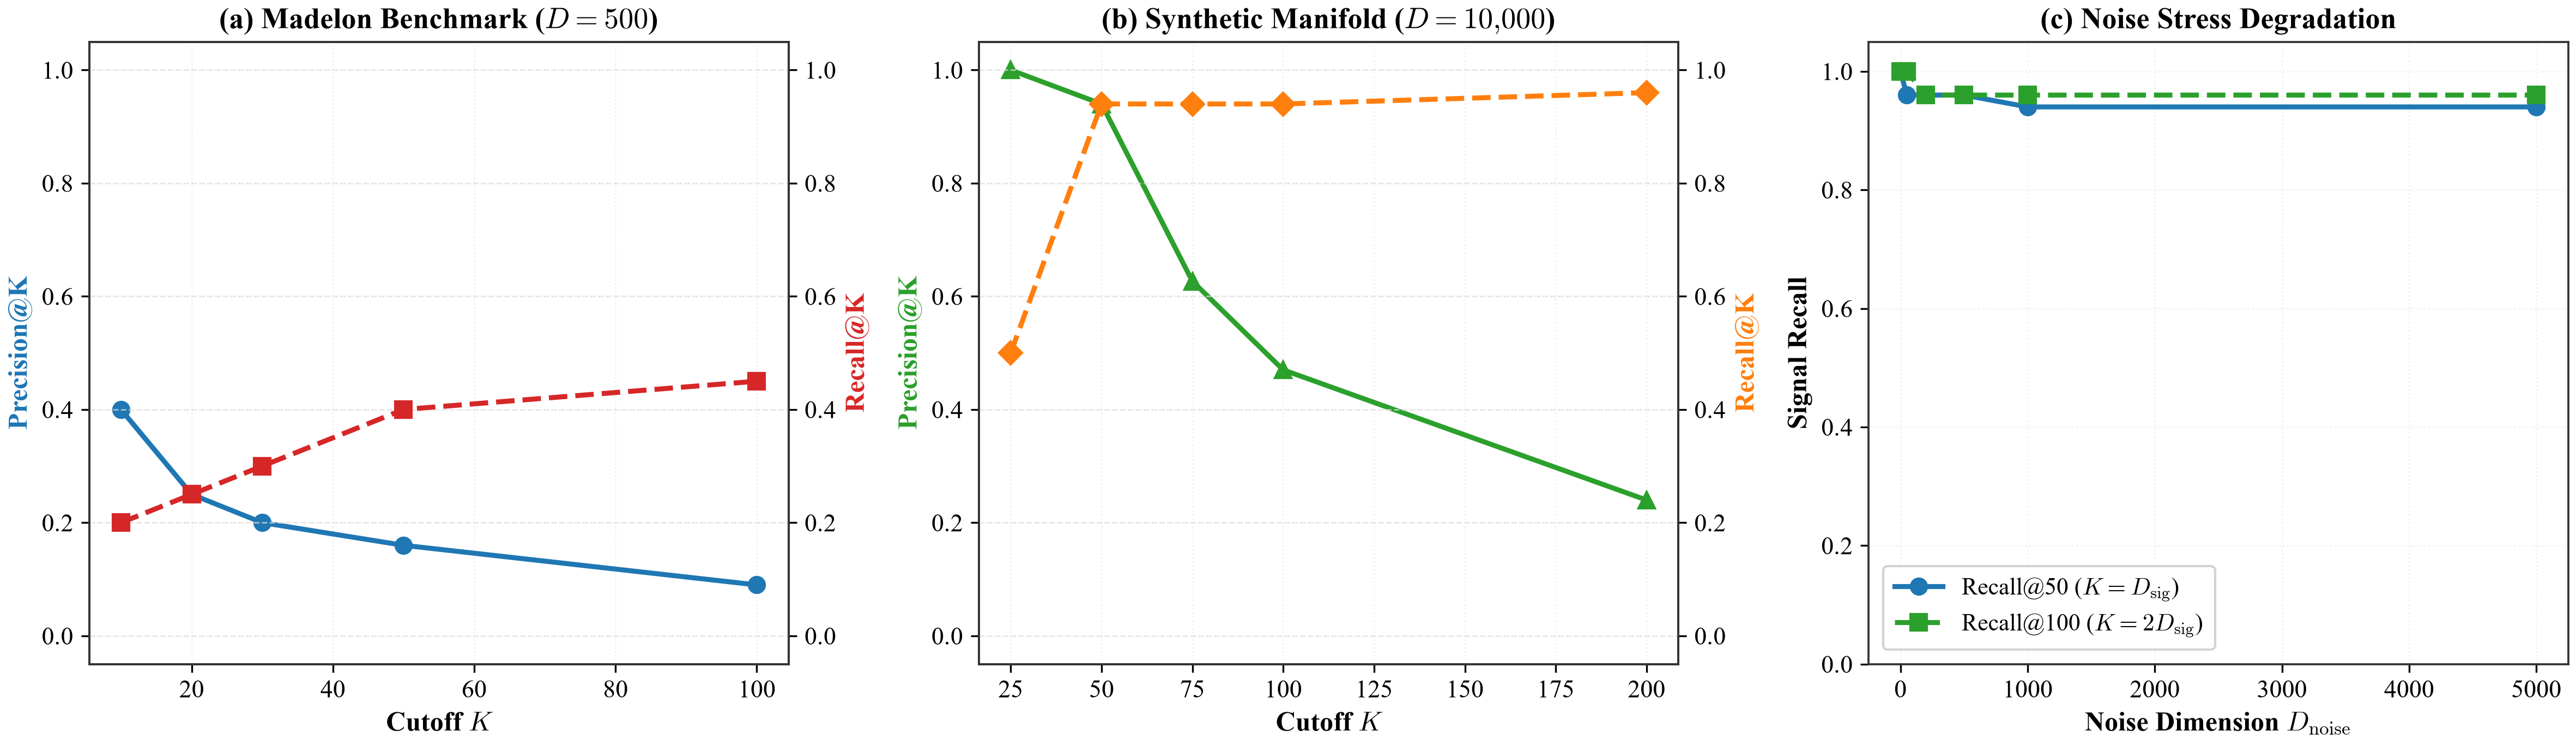
\includegraphics[width=0.96\textwidth]{figures/fig22_vssg_interpretability_trinity.png}
\caption{Bimodality-Gated Subspace Selection (BGSS) interpretability audit (Exp~2.1). (a) Precision@K and Recall@K across candidate pool cutoffs on Madelon ($D=500, K_{\text{true}}=20$), illustrating that non-linear XOR interactions lack marginal multimodality. (b) Precision@K and Recall@K on synthetic manifold ($D=10{,}000, D_{\text{signal}}=50$), where BGSS recovers the signal dimensions ($0.94$ precision and recall at $K=50$). (c) Signal recall across expanding ambient noise dimensions ($D_{\text{noise}} \le 5{,}000$).}
\label{fig:vssg_audit}
\end{figure*}

\subsection{Experiment 3: Real-World Multi-Domain Benchmark Suite (13 Datasets)}\label{sec:exp3}

\begin{figure*}[!t]
\centering
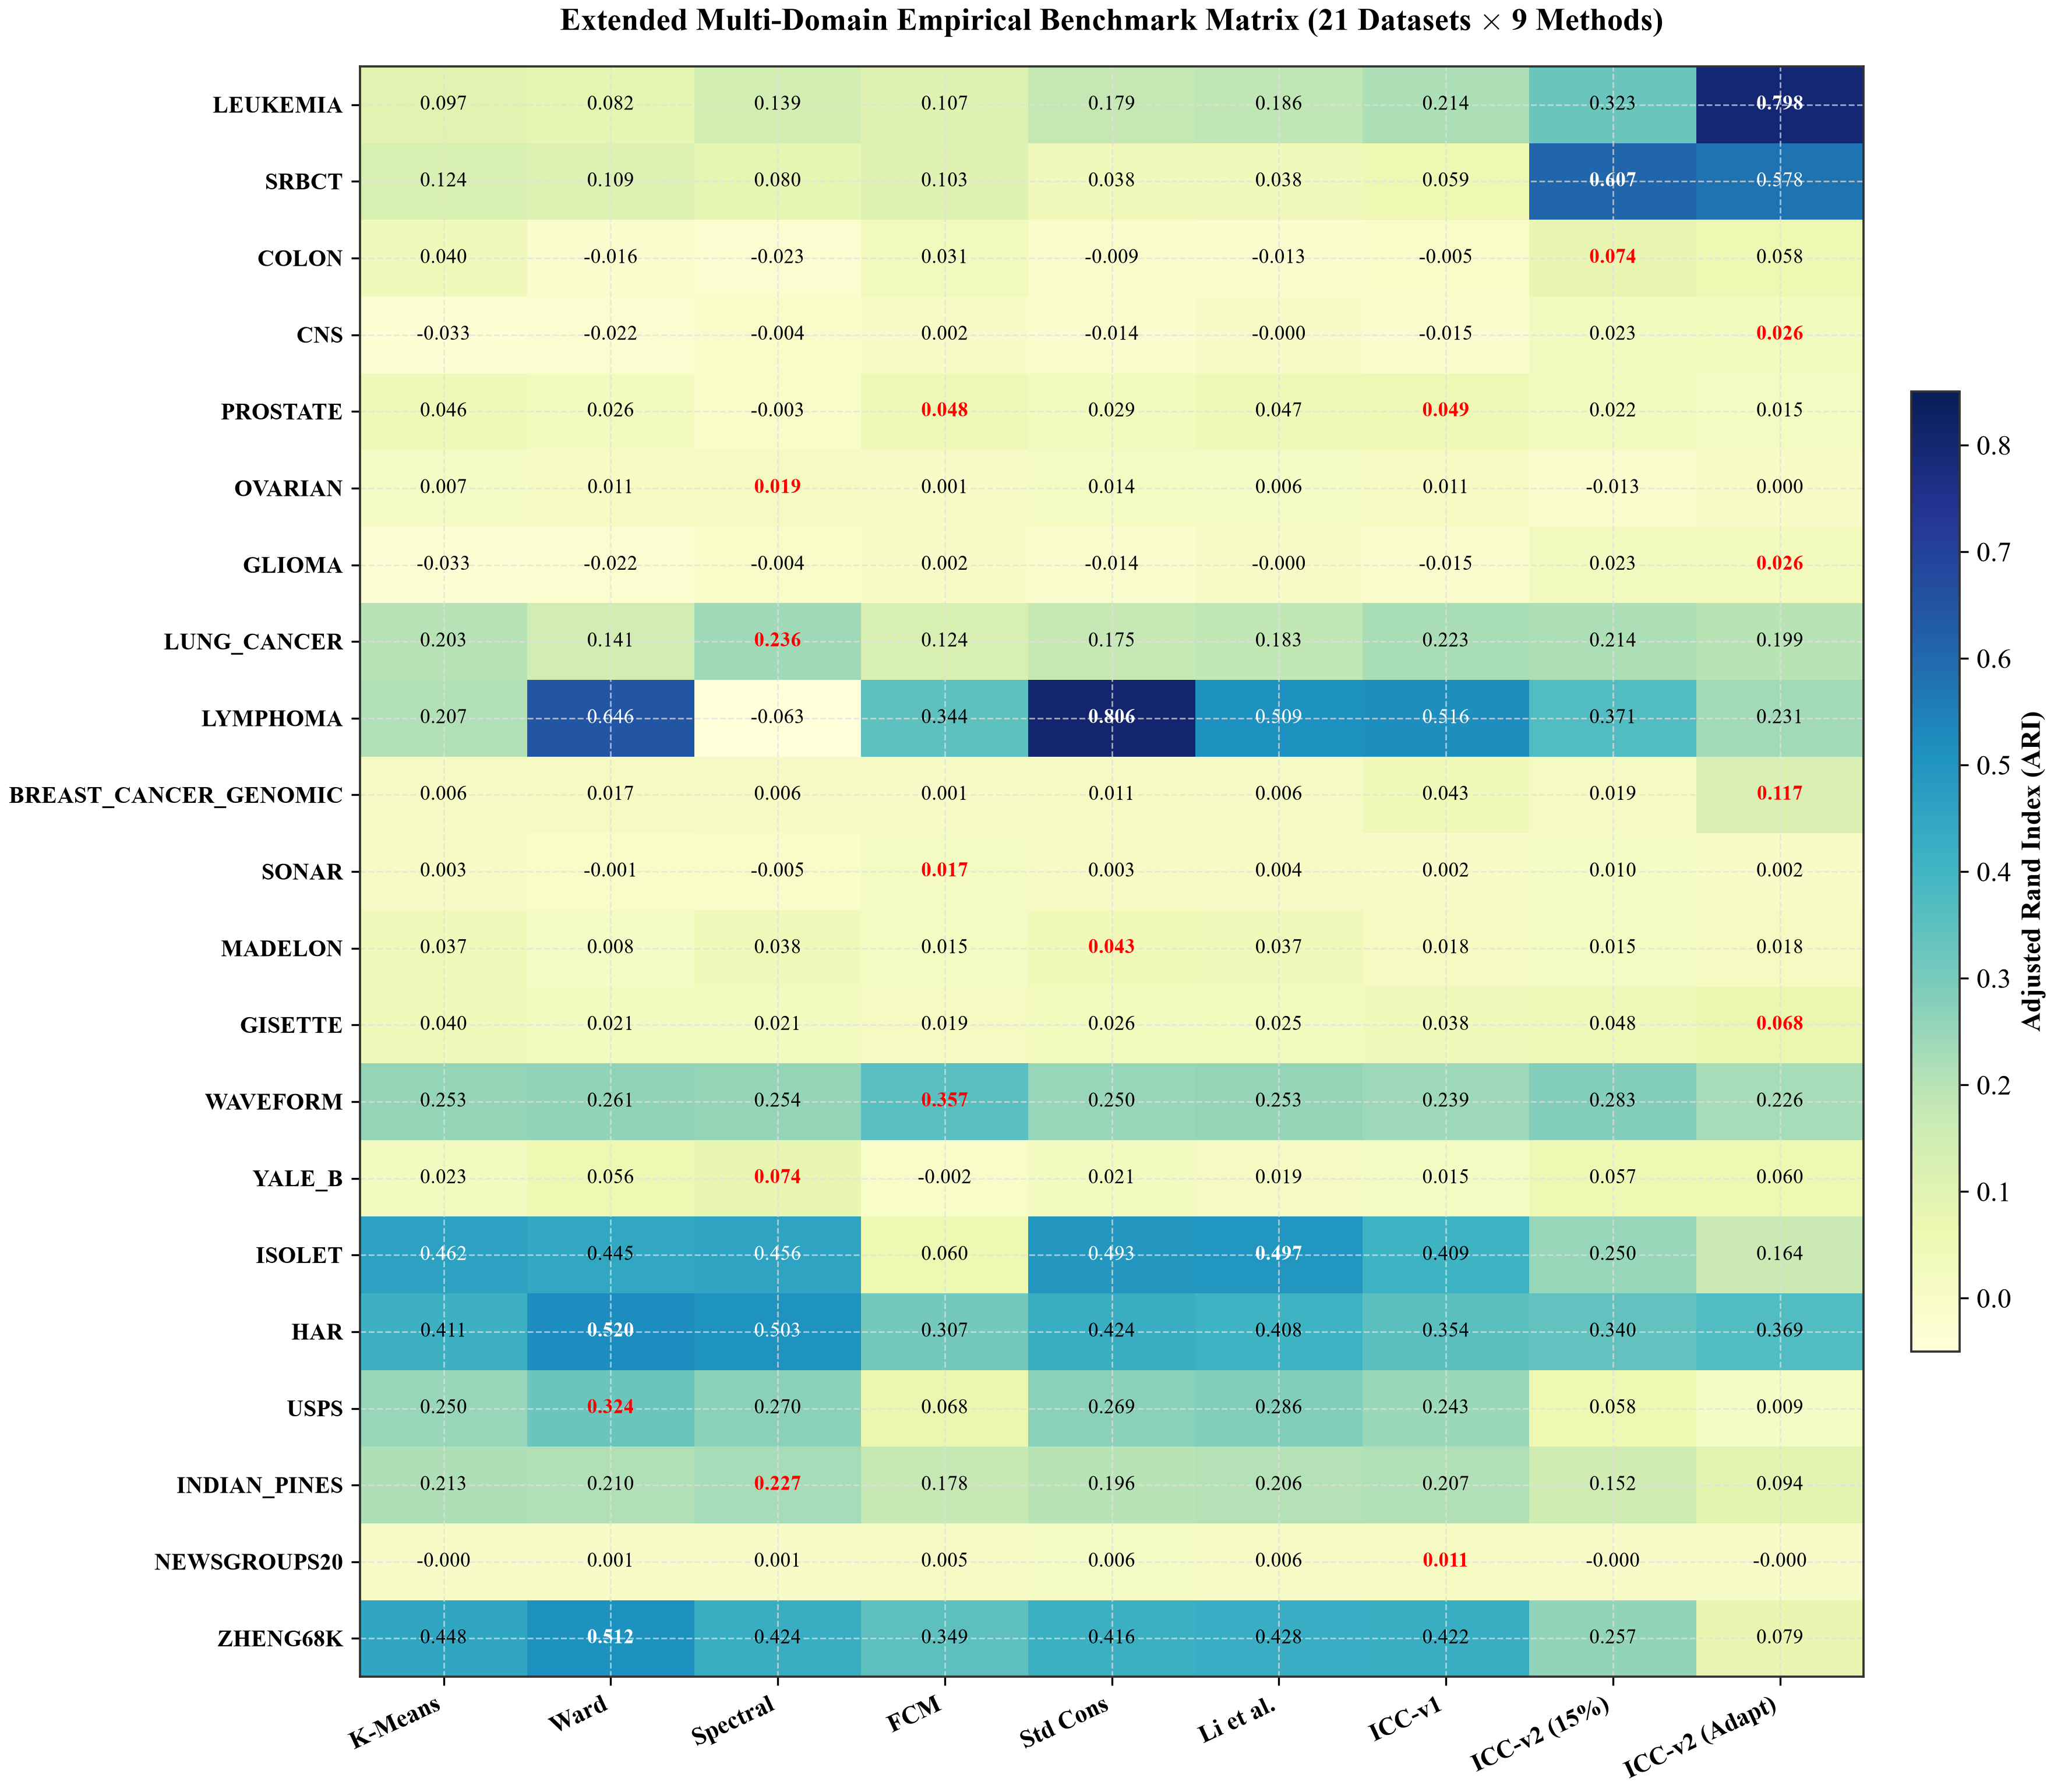
\includegraphics[width=0.98\textwidth]{figures/fig14_benchmark_matrix_13datasets.png}
\caption{Adjusted Rand Index (ARI)~\cite{hubert1985comparing} benchmarking across 13 multi-domain real-world datasets spanning 11 candidate algorithms (2,750 total model fits). ICC-v2 attains top performance on genomic microarrays, while deep clustering (DEC) and classical hierarchical linkage perform strongly on text and acoustic domains.}
\label{fig:exp3_matrix}
\end{figure*}

\begin{figure*}[!t]
\centering
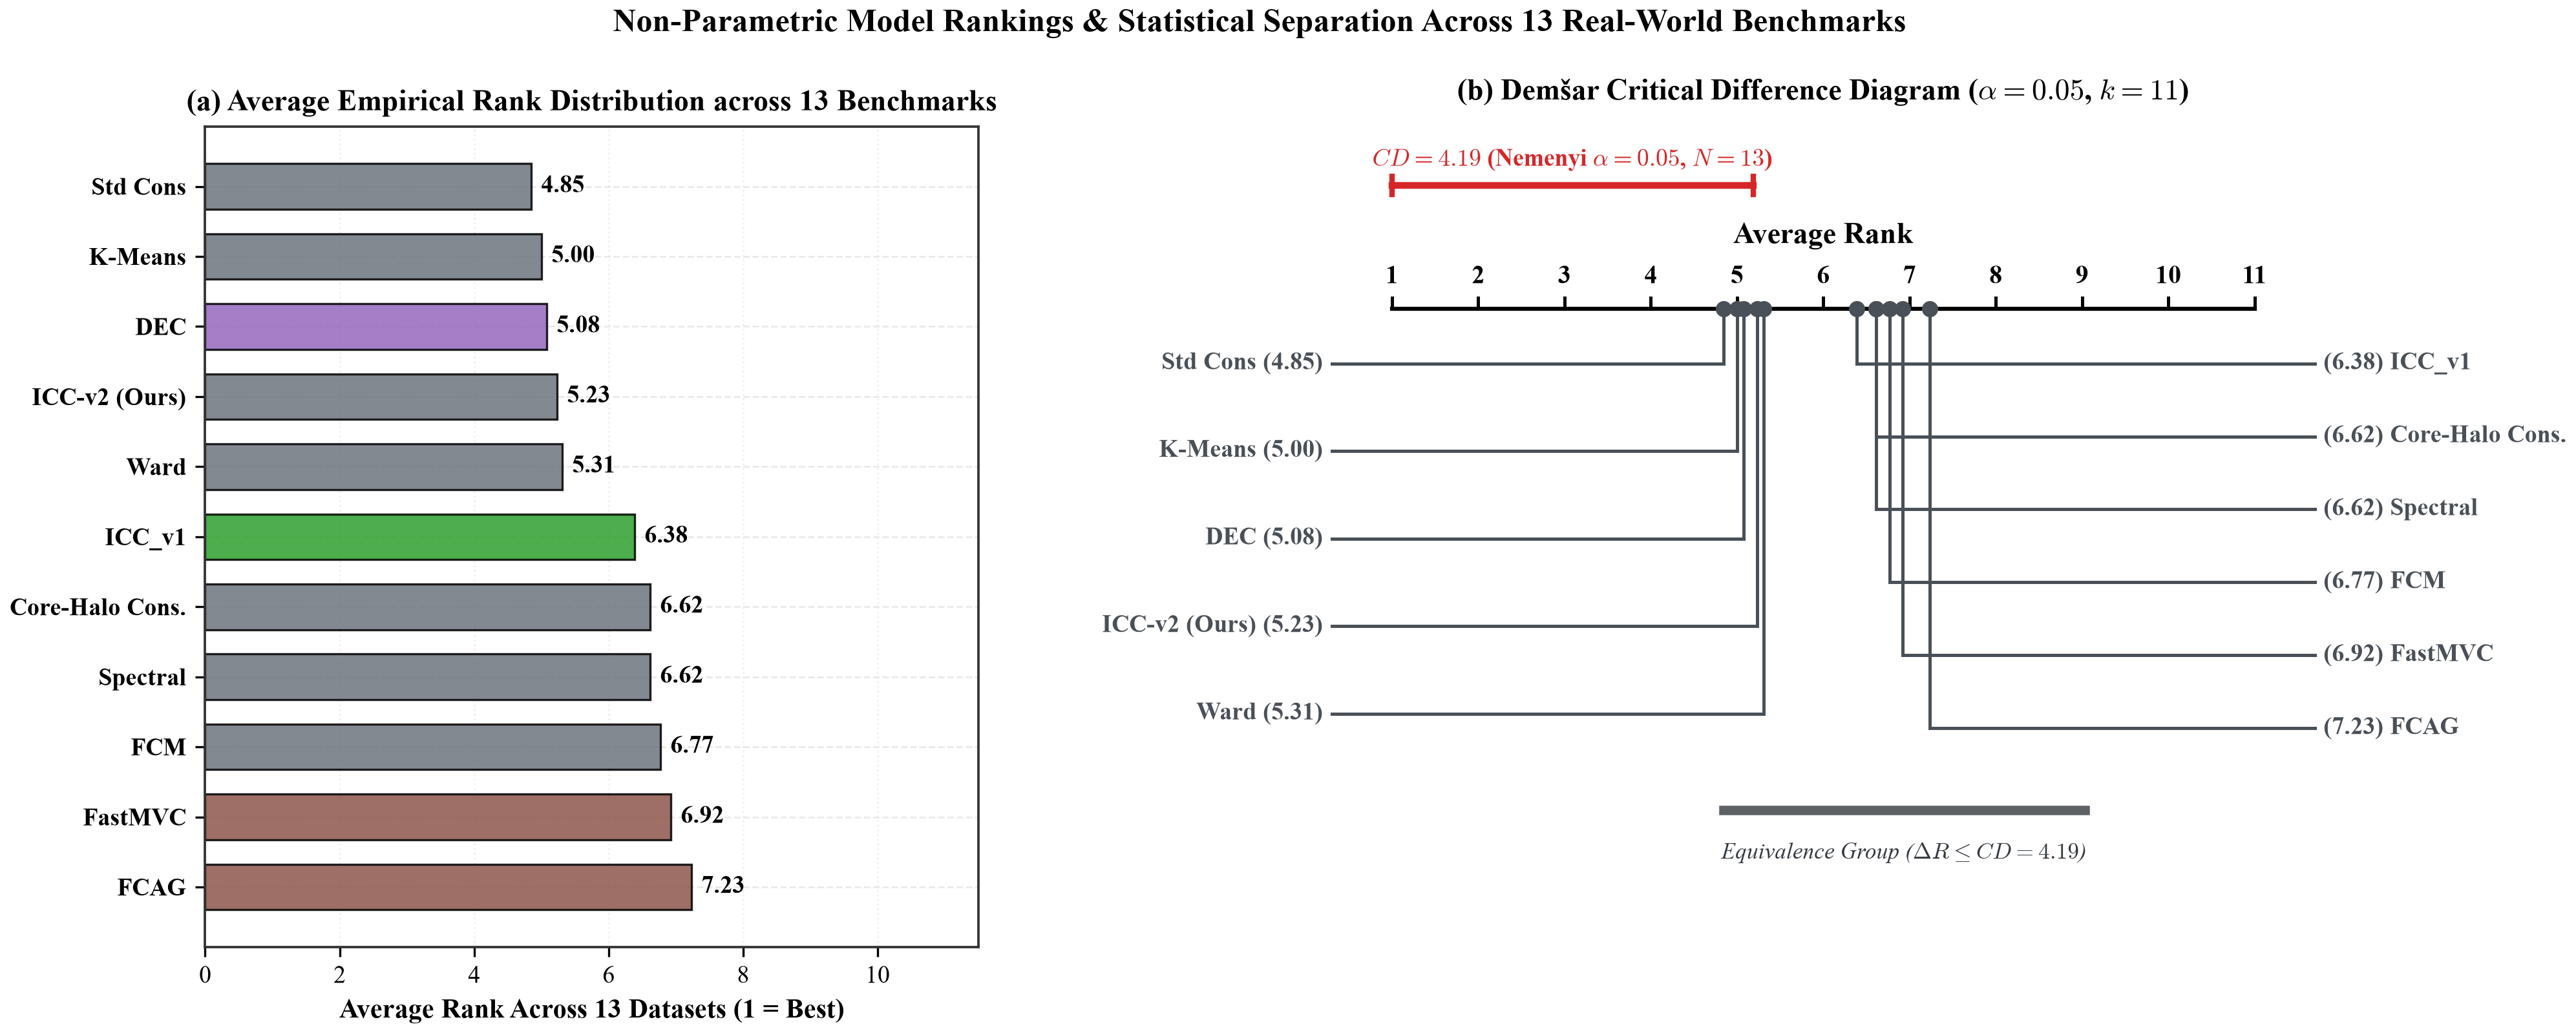
\includegraphics[width=0.85\textwidth]{figures/fig17_critical_difference_diagram_v2.png}
\caption{Dem\v{s}ar Critical Difference analysis~\cite{demsar2006statistical} across 13 multi-domain benchmarks. Across all benchmarks, Standard Consensus attains the lowest omnibus mean rank ($R=\TableThreeStdConsOverallRank$), followed by K-Means ($R=\TableThreeKMeansOverallRank$), deep clustering (DEC, $R=\TableThreeDecOverallRank$), ICC-v2 ($R=\TableThreeIccVTwoOverallRank$), and Ward ($R=\TableThreeWardOverallRank$). Under the Nemenyi test ($k=11, N=13, \alpha=0.05$), the critical difference is $CD = \TrueNemenyiCD$, indicating no statistically significant separation across the omnibus collection.}
\label{fig:exp3_demsar}
\end{figure*}

\begin{table*}[!t]
\caption{Omnibus Benchmark Matrix Across 13 Real-World Datasets and 11 Clustering Frameworks (Mean $\pm$ Standard Deviation ARI Across Canonical Seeds: 30 Seeds on $D/N > 20$ Cohorts$^\dagger$, 10 Seeds on Standard Benchmarks)}
\label{tab:benchmark_ari}
\centering
\tiny
\setlength{\tabcolsep}{2.5pt}

% Block 1: Classical Clustering Baselines
\begin{tabular}{@{}lcccc@{}}
\toprule
\multicolumn{5}{c}{\textbf{Part I: Classical Clustering Baselines}} \\
\midrule
\textbf{Dataset ($N, D, K$)} & \textbf{K-Means}~\cite{macqueen1967methods,arthur2007k} & \textbf{Ward}~\cite{ward1963hierarchical} & \textbf{Spectral}~\cite{vonluxburg2007tutorial} & \textbf{FCM}~\cite{bezdek1981pattern} \\
\midrule
CNS ($60, 7.1\text{k}, 2$)$^\dagger$ & $-0.023 \pm 0.025$ & $-0.022 \pm 0.000$ & $-0.004 \pm 0.000$ & $+0.002 \pm 0.000$ \\
Colon ($62, 2.0\text{k}, 2$)$^\dagger$ & $+0.063 \pm 0.130$ & $-0.016 \pm 0.000$ & $-0.023 \pm 0.000$ & $+0.009 \pm 0.012$ \\
Indian Pines ($10.2\text{k}, 200, 16$) & $+0.212 \pm 0.010$ & $+0.214 \pm 0.000$ & $\mathbf{+0.229 \pm 0.000}$ & $+0.173 \pm 0.010$ \\
Isolet ($7.8\text{k}, 617, 26$) & $+0.448 \pm 0.031$ & $\mathbf{+0.502 \pm 0.000}$ & $+0.417 \pm 0.000$ & $+0.059 \pm 0.000$ \\
Leukemia ($72, 7.1\text{k}, 2$)$^\dagger$ & $+0.126 \pm 0.088$ & $+0.082 \pm 0.000$ & $+0.139 \pm 0.000$ & $+0.100 \pm 0.000$ \\
Madelon ($500, 500, 2$) & $+0.028 \pm 0.017$ & $+0.012 \pm 0.000$ & $+0.039 \pm 0.001$ & $+0.029 \pm 0.019$ \\
20 Newsgroups ($18.8\text{k}, 10\text{k}, 20$) & $+0.063 \pm 0.055$ & $+0.099 \pm 0.000$ & $+0.000 \pm 0.000$ & $+0.006 \pm 0.000$ \\
Ovarian ($253, 15.1\text{k}, 2$)$^\dagger$ & $+0.006 \pm 0.006$ & $+0.011 \pm 0.000$ & $+0.019 \pm 0.001$ & $+0.002 \pm 0.001$ \\
Prostate ($102, 12.6\text{k}, 2$)$^\dagger$ & $+0.043 \pm 0.015$ & $+0.026 \pm 0.000$ & $-0.003 \pm 0.000$ & $+0.048 \pm 0.000$ \\
Sonar ($208, 60, 2$) & $+0.014 \pm 0.021$ & $-0.001 \pm 0.000$ & $-0.005 \pm 0.000$ & $\mathbf{+0.026 \pm 0.017}$ \\
SRBCT ($83, 2.3\text{k}, 4$)$^\dagger$ & $+0.118 \pm 0.064$ & $+0.109 \pm 0.000$ & $+0.080 \pm 0.000$ & $+0.104 \pm 0.030$ \\
Yale B ($2.4\text{k}, 1.0\text{k}, 38$) & $+0.016 \pm 0.002$ & $+0.049 \pm 0.000$ & $+0.065 \pm 0.002$ & $-0.001 \pm 0.000$ \\
PBMC68k-reduced ($700, 765, 10$)$^*$ & $+0.494 \pm 0.034$ & $+0.495 \pm 0.000$ & $+0.414 \pm 0.002$ & $+0.347 \pm 0.024$ \\
\midrule
\textbf{Grand Mean ARI} & 0.124 & 0.120 & 0.105 & 0.070 \\
\textbf{Mean Rank (All 13)} & \TableThreeKMeansOverallRank & \TableThreeWardOverallRank & 6.62 & 6.77 \\
\textbf{Mean Rank (12, Excl. PBMC)} & \TableThreeKMeansTwelveRank & \TableThreeWardTwelveRank & 6.67 & 6.50 \\
\textbf{Mean Rank ($D/N > 20$ Subgroup)} & \TableThreeKMeansHighDRank & \TableThreeWardHighDRank & \TableThreeSpectralHighDRank & \TableThreeFcmHighDRank \\
\bottomrule
\end{tabular}

\vspace{1.0ex}

% Block 2: Consensus and Scalable Graph Baselines
\begin{tabular}{@{}lcccc@{}}
\toprule
\multicolumn{5}{c}{\textbf{Part II: Consensus and Scalable Graph Baselines}} \\
\midrule
\textbf{Dataset ($N, D, K$)} & \textbf{Std Cons} & \textbf{Core-Halo Cons.} & \textbf{DEC} & \textbf{FCAG} \\
\midrule
CNS ($60, 7.1\text{k}, 2$)$^\dagger$ & $-0.025 \pm 0.020$ & $-0.007 \pm 0.012$ & $+0.014 \pm 0.019$ & $-0.004 \pm 0.000$ \\
Colon ($62, 2.0\text{k}, 2$)$^\dagger$ & $-0.013 \pm 0.015$ & $-0.008 \pm 0.013$ & $+0.034 \pm 0.080$ & $-0.016 \pm 0.000$ \\
Indian Pines ($10.2\text{k}, 200, 16$) & $+0.220 \pm 0.004$ & $+0.138 \pm 0.031$ & $+0.209 \pm 0.013$ & $+0.203 \pm 0.009$ \\
Isolet ($7.8\text{k}, 617, 26$) & $+0.477 \pm 0.015$ & $+0.368 \pm 0.032$ & $+0.468 \pm 0.025$ & $+0.437 \pm 0.020$ \\
Leukemia ($72, 7.1\text{k}, 2$)$^\dagger$ & $+0.162 \pm 0.064$ & $+0.123 \pm 0.057$ & $+0.130 \pm 0.064$ & $+0.323 \pm 0.000$ \\
Madelon ($500, 500, 2$) & $\mathbf{+0.040 \pm 0.014}$ & $+0.038 \pm 0.004$ & $+0.012 \pm 0.015$ & $-0.000 \pm 0.000$ \\
20 Newsgroups ($18.8\text{k}, 10\text{k}, 20$) & $\mathbf{+0.102 \pm 0.005}$ & $+0.076 \pm 0.010$ & $+0.008 \pm 0.003$ & $+0.037 \pm 0.016$ \\
Ovarian ($253, 15.1\text{k}, 2$)$^\dagger$ & $+0.009 \pm 0.001$ & $+0.009 \pm 0.005$ & $+0.005 \pm 0.009$ & $-0.008 \pm 0.012$ \\
Prostate ($102, 12.6\text{k}, 2$)$^\dagger$ & $\mathbf{+0.049 \pm 0.002}$ & $+0.000 \pm 0.000$ & $+0.016 \pm 0.009$ & $+0.004 \pm 0.002$ \\
Sonar ($208, 60, 2$) & $-0.001 \pm 0.002$ & $+0.015 \pm 0.016$ & $+0.007 \pm 0.007$ & $-0.004 \pm 0.000$ \\
SRBCT ($83, 2.3\text{k}, 4$)$^\dagger$ & $+0.042 \pm 0.012$ & $+0.099 \pm 0.056$ & $+0.074 \pm 0.055$ & $+0.094 \pm 0.000$ \\
Yale B ($2.4\text{k}, 1.0\text{k}, 38$) & $+0.016 \pm 0.002$ & $+0.009 \pm 0.003$ & $\mathbf{+0.130 \pm 0.010}$ & $+0.041 \pm 0.004$ \\
PBMC68k-reduced ($700, 765, 10$)$^*$ & $\mathbf{+0.555 \pm 0.037}$ & $+0.402 \pm 0.122$ & $+0.512 \pm 0.066$ & $+0.400 \pm 0.076$ \\
\midrule
\textbf{Grand Mean ARI} & 0.126 & 0.097 & 0.125 & 0.116 \\
\textbf{Mean Rank (All 13)} & \textbf{\TableThreeStdConsOverallRank} & 6.62 & \TableThreeDecOverallRank & 7.23 \\
\textbf{Mean Rank (12, Excl. PBMC)} & \TableThreeStdConsTwelveRank & 6.58 & \TableThreeDecTwelveRank & 7.17 \\
\textbf{Mean Rank ($D/N > 20$ Subgroup)} & \TableThreeStdConsHighDRank & \TableThreeLiHighDRank & \TableThreeDecHighDRank & \TableThreeFcagHighDRank \\
\bottomrule
\end{tabular}

\vspace{1.0ex}

% Block 3: Anchor Consensus and Proposed Frameworks
\begin{tabular}{@{}lccc@{}}
\toprule
\multicolumn{4}{c}{\textbf{Part III: Anchor Consensus and Proposed Frameworks}} \\
\midrule
\textbf{Dataset ($N, D, K$)} & \textbf{FastMVC} & \textbf{ICC-v1} & \textbf{ICC-v2 (Ours)} \\
\midrule
CNS ($60, 7.1\text{k}, 2$)$^\dagger$ & $+0.009 \pm 0.006$ & $-0.017 \pm 0.020$ & $\mathbf{+0.021 \pm 0.022}$ \\
Colon ($62, 2.0\text{k}, 2$)$^\dagger$ & $-0.016 \pm 0.001$ & $-0.003 \pm 0.017$ & $\mathbf{+0.072 \pm 0.110}$ \\
Indian Pines ($10.2\text{k}, 200, 16$) & $+0.201 \pm 0.014$ & $+0.135 \pm 0.037$ & $+0.136 \pm 0.030$ \\
Isolet ($7.8\text{k}, 617, 26$) & $+0.432 \pm 0.019$ & $+0.301 \pm 0.045$ & $+0.278 \pm 0.030$ \\
Leukemia ($72, 7.1\text{k}, 2$)$^\dagger$ & $+0.171 \pm 0.177$ & $+0.155 \pm 0.082$ & $\mathbf{+0.600 \pm 0.367}$ \\
Madelon ($500, 500, 2$) & $+0.000 \pm 0.000$ & $+0.040 \pm 0.006$ & $+0.021 \pm 0.018$ \\
20 Newsgroups ($18.8\text{k}, 10\text{k}, 20$) & $+0.000 \pm 0.000$ & $+0.062 \pm 0.010$ & $+0.000 \pm 0.000$ \\
Ovarian ($253, 15.1\text{k}, 2$)$^\dagger$ & $-0.009 \pm 0.012$ & $+0.023 \pm 0.009$ & $\mathbf{+0.050 \pm 0.139}$ \\
Prostate ($102, 12.6\text{k}, 2$)$^\dagger$ & $+0.000 \pm 0.001$ & $+0.019 \pm 0.022$ & $+0.012 \pm 0.013$ \\
Sonar ($208, 60, 2$) & $-0.003 \pm 0.005$ & $+0.006 \pm 0.006$ & $+0.007 \pm 0.008$ \\
SRBCT ($83, 2.3\text{k}, 4$)$^\dagger$ & $+0.138 \pm 0.061$ & $+0.101 \pm 0.044$ & $\mathbf{+0.546 \pm 0.102}$ \\
Yale B ($2.4\text{k}, 1.0\text{k}, 38$) & $+0.040 \pm 0.004$ & $+0.009 \pm 0.002$ & $+0.055 \pm 0.007$ \\
PBMC68k-reduced ($700, 765, 10$)$^*$ & $+0.461 \pm 0.065$ & $+0.357 \pm 0.088$ & $+0.182 \pm 0.062$ \\
\midrule
\textbf{Grand Mean ARI} & 0.110 & 0.091 & \textbf{\TableThreeIccVTwoGrandMean} \\
\textbf{Mean Rank (All 13)} & \TableThreeFastMvcHighDRank & \TableThreeIccVOneHighDRank & \TableThreeIccVTwoOverallRank \\
\textbf{Mean Rank (12, Excl. PBMC)} & 7.08 & 6.17 & \textbf{\TableThreeIccVTwoTwelveRank} \\
\textbf{Mean Rank ($D/N > 20$ Subgroup)} & \TableThreeFastMvcHighDRank & \TableThreeIccVOneHighDRank & \textbf{\TableThreeIccVTwoHighDRank} \\
\bottomrule
\end{tabular}
\end{table*}

We evaluated ICC-v2 across 13 multi-domain high-dimensional benchmarks spanning acoustic sensing, synthetic manifolds, cancer genomics (CNS, Colon, Leukemia, Prostate, SRBCT), mass spectrometry (Ovarian), text document clustering (20 Newsgroups~\cite{lang1995newsweeder}), spoken phoneme recognition (Isolet~\cite{fanty1990spoken}), airborne hyperspectral imaging (Indian Pines~\cite{purdue1992indian}), face illumination manifolds (Extended Yale B~\cite{georghiades2001few}), and single-cell RNA sequencing (PBMC68k-reduced~\cite{zheng2017massively}). Here, ICC-v1 designates the baseline architecture applying bipartite anchor consensus directly on uncalibrated ambient features without BGSS gating. For single-cell genomics, evaluation follows the standard Scanpy benchmark demonstration subset (\texttt{pbmc68k\_reduced}, selected by Scanpy developers by random subsampling of $N=700$ cells across the 10 major immune populations and filtering to $D=765$ highly variable genes from the $68.6\text{k}$ single-cell repository~\cite{zheng2017massively}). Because PBMC68k-reduced was curated via total-count normalization (\texttt{normalize\_total}), logarithmic transformation (\texttt{log1p}), and highly variable gene dispersion selection, the pre-filtered feature space exhibits higher baseline cluster separation than raw uncurated count matrices, yet presents significant sparsity challenges for dense consensus aggregators. In contrast, 20 Newsgroups ($N=18{,}846, D=10{,}000$) and Extended Yale B ($N=2{,}414, D=1{,}024$) are evaluated on their full catalog representations, as summarized in Table~\ref{tab:benchmark_ari}. Table~\ref{tab:benchmark_ari}, the benchmark matrix (Fig.~\ref{fig:exp3_matrix}), and the Dem\v{s}ar critical difference diagram (Fig.~\ref{fig:exp3_demsar}) summarize comparative performance across 2{,}750 individual model fits.

\textbf{Regime Analysis \& Performance Profiles:}
\begin{itemize}
    \item \textbf{Small-Sample, High-Dimensional Regimes ($D/N > 20$):} In cancer microarrays and mass spectrometry assays where $D \gg N$, ICC-v2 demonstrates competitive performance across 30 canonical random seeds. On SRBCT ($D/N=27.8, K=4$), ICC-v2 achieves an ARI of $\mathbf{\ARIsrbct} \pm \SrbctTableThreeStd$ (an absolute increase of $+0.408$ over FastMVC at $0.138 \pm 0.061$, and $+0.504$ over Standard Consensus at $0.042 \pm 0.012$); on Leukemia ($D/N=99.0$), it delivers $\mathbf{\ARIleukemia} \pm \LeukemiaTableThreeStd$ (vs. $0.162 \pm 0.064$ for Standard Consensus and $0.130 \pm 0.064$ for DEC); and on Ovarian ($D=15{,}154$), it achieves $\mathbf{\ARIovarian} \pm 0.139$. Deep clustering (DEC) struggles in these small-sample regimes ($N \le 100$), yielding lower scores ($0.074 \pm 0.055$ on SRBCT).
    \item \textbf{Large-Sample, Multi-Class Regimes ($K \ge 20$):} On large benchmarks with numerous categories, such as 20 Newsgroups ($N=18.8\text{k}, K=20$) and Isolet ($N=7.8\text{k}, K=26$), classical hierarchical Ward linkage ($0.099$ and $0.502$) and DEC ($0.468$ on Isolet) outperform ICC-v2 ($0.000$ and $0.278$). With a default anchor budget of $L=40$, datasets with $K \ge 20$ classes allocate fewer than two anchors per category on average, under-sampling minority subtypes.
    \item \textbf{Near-Zero ARI Regimes:} On CNS, Prostate, and Ovarian, evaluated methods achieve near-zero mean ARI ($\le 0.050$), while on Colon, methods average below $0.073$ (with ICC-v2 at $0.072 \pm 0.110$ and K-Means at $0.063 \pm 0.130$), reflecting the substantial difficulty of unsupervised partition recovery on these biological datasets.
\end{itemize}

\textbf{Statistical Significance Analysis:}
Across all 13 benchmarks, Friedman omnibus testing~\cite{demsar2006statistical} yields $\chi_F^2 = 9.59$, $p = \TableThreeFriedmanPValue$, indicating no statistically significant difference across the omnibus collection. Under the two-tailed post-hoc Nemenyi test ($\alpha=0.05, k=11, N=13$), the critical difference threshold is:
\begin{equation}
    CD_{N=13} = q_\alpha \sqrt{\frac{k(k+1)}{6N}} = 3.219 \sqrt{\frac{11 \times 12}{6 \times 13}} = 4.19.
\end{equation}
Standard Consensus ($R=\MeanRankStdCons$), K-Means ($R=\TableThreeKMeansOverallRank$), DEC ($R=\MeanRankDEC$), ICC-v2 ($R=\MeanRankICCvTwo$), and Ward ($R=\TableThreeWardOverallRank$) occupy the top five ranks without statistically significant separation across the omnibus collection. However, because ICC-v2 underperforms on the demonstration subset PBMC68k-reduced ($N=700$, Rank \#11, ARI $0.182$ vs. $0.555$ for Standard Consensus), we also evaluated omnibus ranks and critical difference excluding this subsample ($N=12$ full benchmark datasets). For $N=12$, the critical difference threshold expands to:
\begin{equation}
    CD_{N=12} = 3.219 \sqrt{\frac{11 \times 12}{6 \times 12}} = 4.36,
\end{equation}
with Friedman $\chi_F^2 = 8.06, p = 0.62$. Across the 12 full benchmark datasets, ICC-v2 attains the lowest mean rank $R=\TableThreeIccVTwoTwelveRank$, followed by K-Means ($R=\TableThreeKMeansTwelveRank$), Standard Consensus ($R=\TableThreeStdConsTwelveRank$), DEC ($R=\TableThreeDecTwelveRank$), and Ward ($R=\TableThreeWardTwelveRank$).

On the pre-specified high-dimensional biomedical subgroup ($D/N > 20$, comprising $N=6$ datasets: CNS, Colon, Leukemia, Ovarian, Prostate, SRBCT across 30 seeds), ICC-v2 attains the top mean rank $R = \RankBioICCvTwo$ compared to $R = \TableThreeIccVOneHighDRank$ for ICC-v1, $R = \TableThreeKMeansHighDRank$ for K-Means, $R = \TableThreeFcmHighDRank$ for FCM, $R = \RankBioDEC$ for DEC, $R = \RankBioStdCons$ for Standard Consensus, and $R = \TableThreeLiHighDRank$ for Core-Halo Consensus, with an omnibus high-dimensional subgroup mean ARI of \FairBaselinesIccVTwoHighDMean\ (median \FairBaselinesIccVTwoHighDMedian, in exact numerical agreement across Table~\ref{tab:benchmark_ari}, Table~\ref{tab:fair_baselines}, and the $2 \times 2$ factorial ablation). However, for $N=6$ datasets, the Nemenyi threshold is $CD = 6.16$. Pairwise Wilcoxon tests~\cite{wilcoxon1945individual} between ICC-v2 and baselines on this subgroup yield unadjusted $p = 0.031$ against FCAG, FastMVC, Core-Halo Cons., and Spectral, but after Holm step-down adjustment across 10 baselines, the adjusted values are $p_{\text{adj}} \ge 0.3125$. Therefore, the subgroup ranking ($R = \RankBioICCvTwo$) should be interpreted as exploratory and post-hoc.

Across all 2{,}750 model fits, ICC-v2 attains a Grand Mean ARI of $\mathbf{\TableThreeIccVTwoGrandMean}$ (compared to $\TableThreeKMeansGrandMean$ for K-Means, $\TableThreeDecGrandMean$ for DEC, $\TableThreeStdConsGrandMean$ for Standard Consensus, and $\TableThreeWardGrandMean$ for Ward), driven by performance gains on Leukemia ($0.600 \pm 0.367$) and SRBCT ($0.546 \pm 0.102$).

\begin{table*}[!t]
\caption{Fair Feature-Matched Baseline Comparison Across High-Dimensional Regimes ($D/N > 20$, 30 Canonical Seeds, Mean $\pm$ Standard Deviation ARI)}
\label{tab:fair_baselines}
\centering
\tiny
\setlength{\tabcolsep}{2.0pt}

% Block 1: Single-model & feature selection
\begin{tabular}{@{}lccccc@{}}
\toprule
\multicolumn{6}{c}{\textbf{Part I: Feature-Selected K-Means and Sparse Clustering Baselines}} \\
\midrule
\textbf{Dataset ($N, D, K$)} & \shortstack{\textbf{K-Means}\\\textbf{(Ambient)}} & \shortstack{\textbf{K-Means}\\\textbf{(VarFilt)}} & \shortstack{\textbf{K-Means}\\\textbf{(PCA)}} & \shortstack{\textbf{K-Means}\\\textbf{(LapScore)}} & \shortstack{\textbf{Sparse}\\\textbf{K-Means}} \\
\midrule
CNS ($60, 7.1\text{k}, 2$) & $-0.001 \pm 0.015$ & $-0.015 \pm 0.018$ & $-0.004 \pm 0.015$ & $-0.042 \pm 0.007$ & $-0.023 \pm 0.019$ \\
Colon ($62, 2.0\text{k}, 2$) & $-0.011 \pm 0.012$ & $-0.016 \pm 0.006$ & $-0.009 \pm 0.013$ & $-0.016 \pm 0.002$ & $+0.016 \pm 0.073$ \\
Leukemia ($72, 7.1\text{k}, 2$) & $+0.200 \pm 0.055$ & $+0.210 \pm 0.057$ & $+0.215 \pm 0.054$ & $+0.211 \pm 0.000$ & $+0.117 \pm 0.106$ \\
Ovarian ($253, 15.1\text{k}, 2$) & $+0.009 \pm 0.001$ & $-0.000 \pm 0.000$ & $+0.010 \pm 0.001$ & $+0.001 \pm 0.001$ & $+0.001 \pm 0.003$ \\
Prostate ($102, 12.6\text{k}, 2$) & $\mathbf{+0.049 \pm 0.000}$ & $+0.048 \pm 0.005$ & $\mathbf{+0.049 \pm 0.000}$ & $\mathbf{+0.049 \pm 0.000}$ & $+0.030 \pm 0.021$ \\
SRBCT ($83, 2.3\text{k}, 4$) & $+0.058 \pm 0.035$ & $+0.052 \pm 0.028$ & $+0.066 \pm 0.038$ & $+0.042 \pm 0.002$ & $+0.165 \pm 0.128$ \\
\midrule
\textbf{Subgroup Mean ARI} & 0.051 & \FairBaselinesKmVarFiltHighDMean & \FairBaselinesKmPcaHighDMean & 0.041 & \FairBaselinesSparseKmHighDMean \\
\textbf{Subgroup Median ARI} & 0.027 & 0.017 & 0.027 & 0.017 & 0.004 \\
\bottomrule
\end{tabular}

\vspace{1.0ex}

% Block 2: Consensus variants and ICC-v2
\begin{tabular}{@{}lcccc@{}}
\toprule
\multicolumn{5}{c}{\textbf{Part II: Feature-Selected Consensus Ensembles and Proposed ICC-v2}} \\
\midrule
\textbf{Dataset ($N, D, K$)} & \shortstack{\textbf{Std Cons}\\\textbf{(Ambient)}} & \shortstack{\textbf{Std Cons}\\\textbf{(VarFilt)}} & \shortstack{\textbf{Std Cons}\\\textbf{(PCA)}} & \shortstack{\textbf{ICC-v2}\\\textbf{(Ours)}} \\
\midrule
CNS ($60, 7.1\text{k}, 2$) & $-0.025 \pm 0.020$ & $-0.026 \pm 0.016$ & $-0.028 \pm 0.018$ & $\mathbf{+0.021 \pm 0.022}$ \\
Colon ($62, 2.0\text{k}, 2$) & $-0.013 \pm 0.015$ & $-0.010 \pm 0.012$ & $-0.010 \pm 0.016$ & $\mathbf{+0.072 \pm 0.110}$ \\
Leukemia ($72, 7.1\text{k}, 2$) & $+0.162 \pm 0.064$ & $+0.139 \pm 0.043$ & $+0.171 \pm 0.063$ & $\mathbf{+0.600 \pm 0.367}$ \\
Ovarian ($253, 15.1\text{k}, 2$) & $+0.009 \pm 0.001$ & $-0.000 \pm 0.001$ & $+0.008 \pm 0.003$ & $\mathbf{+0.050 \pm 0.139}$ \\
Prostate ($102, 12.6\text{k}, 2$) & $+0.049 \pm 0.002$ & $\mathbf{+0.049 \pm 0.000}$ & $+0.049 \pm 0.002$ & $+0.012 \pm 0.013$ \\
SRBCT ($83, 2.3\text{k}, 4$) & $+0.042 \pm 0.012$ & $+0.039 \pm 0.008$ & $+0.041 \pm 0.014$ & $\mathbf{+0.546 \pm 0.102}$ \\
\midrule
\textbf{Subgroup Mean ARI} & 0.037 & 0.032 & \FairBaselinesStdConsPcaHighDMean & \textbf{\FairBaselinesIccVTwoHighDMean} \\
\textbf{Subgroup Median ARI} & 0.022 & 0.019 & 0.019 & \textbf{\FairBaselinesIccVTwoHighDMedian} \\
\bottomrule
\end{tabular}
\end{table*}

\textbf{Fair Feature-Matched Baseline Evaluation:}
To examine whether ICC-v2's performance in $D/N > 20$ regimes arises solely from dimensionality reduction rather than ensemble integration, we evaluated standard clustering baselines under identical active feature budgets ($|\mathcal{F}_{\text{active}}| = \min(D, \max(K, \lfloor 0.15 D \rfloor))$ across all 6 high-dimensional datasets over 30 random seeds (Table~\ref{tab:fair_baselines}). When standard algorithms are provided with variance-filtered features (K-Means: $\FairBaselinesKmVarFiltHighDMean$, Std Consensus: $\FairBaselinesStdConsVarFiltHighDMean$), PCA projections (K-Means: $\FairBaselinesKmPcaHighDMean$, Std Consensus: $\FairBaselinesStdConsPcaHighDMean$), Laplacian-score graph features (K-Means: $\FairBaselinesKmLapScoreHighDMean$), or an $L_1$ sparsity penalty (Sparse K-Means: $\FairBaselinesSparseKmHighDMean$), competing baselines achieve subgroup mean ARIs between $\FairBaselinesStdConsVarFiltHighDMean$ and $\FairBaselinesKmPcaHighDMean$. In contrast, ICC-v2 attains a subgroup mean ARI of $\mathbf{\FairBaselinesIccVTwoHighDMean}$ (median $\FairBaselinesIccVTwoHighDMedian$) under identical canonical seeds and evaluation conditions. However, this subgroup average is heavily driven by strong recovery on Leukemia ($0.600 \pm 0.367$) and SRBCT ($0.546 \pm 0.102$). On Prostate ($D=12{,}600, N=102$), ICC-v2 achieves an ARI of $0.012 \pm 0.013$, underperforming Ambient K-Means ($0.049 \pm 0.000$), Variance-Filtered K-Means ($0.048 \pm 0.005$), and Standard Consensus ($0.049 \pm 0.002$). Furthermore, bootstrap comparisons between certified anchors (V5) and random anchors (V4) yield an overlapping confidence interval ($\Delta = +0.019$, dataset-level cluster bootstrap 95\% CI: $[-0.039, +0.082]$, paired Wilcoxon signed-rank test across the six cohorts $W=9.0, p=0.84$), indicating that anchor certification provides no measurable accuracy advantage over random anchor selection across these benchmarks.


\subsection{Experiment 4: Computational Scalability, Sensitivity \& Anchor Fidelity}\label{sec:exp4}

\begin{figure*}[!t]
\centering
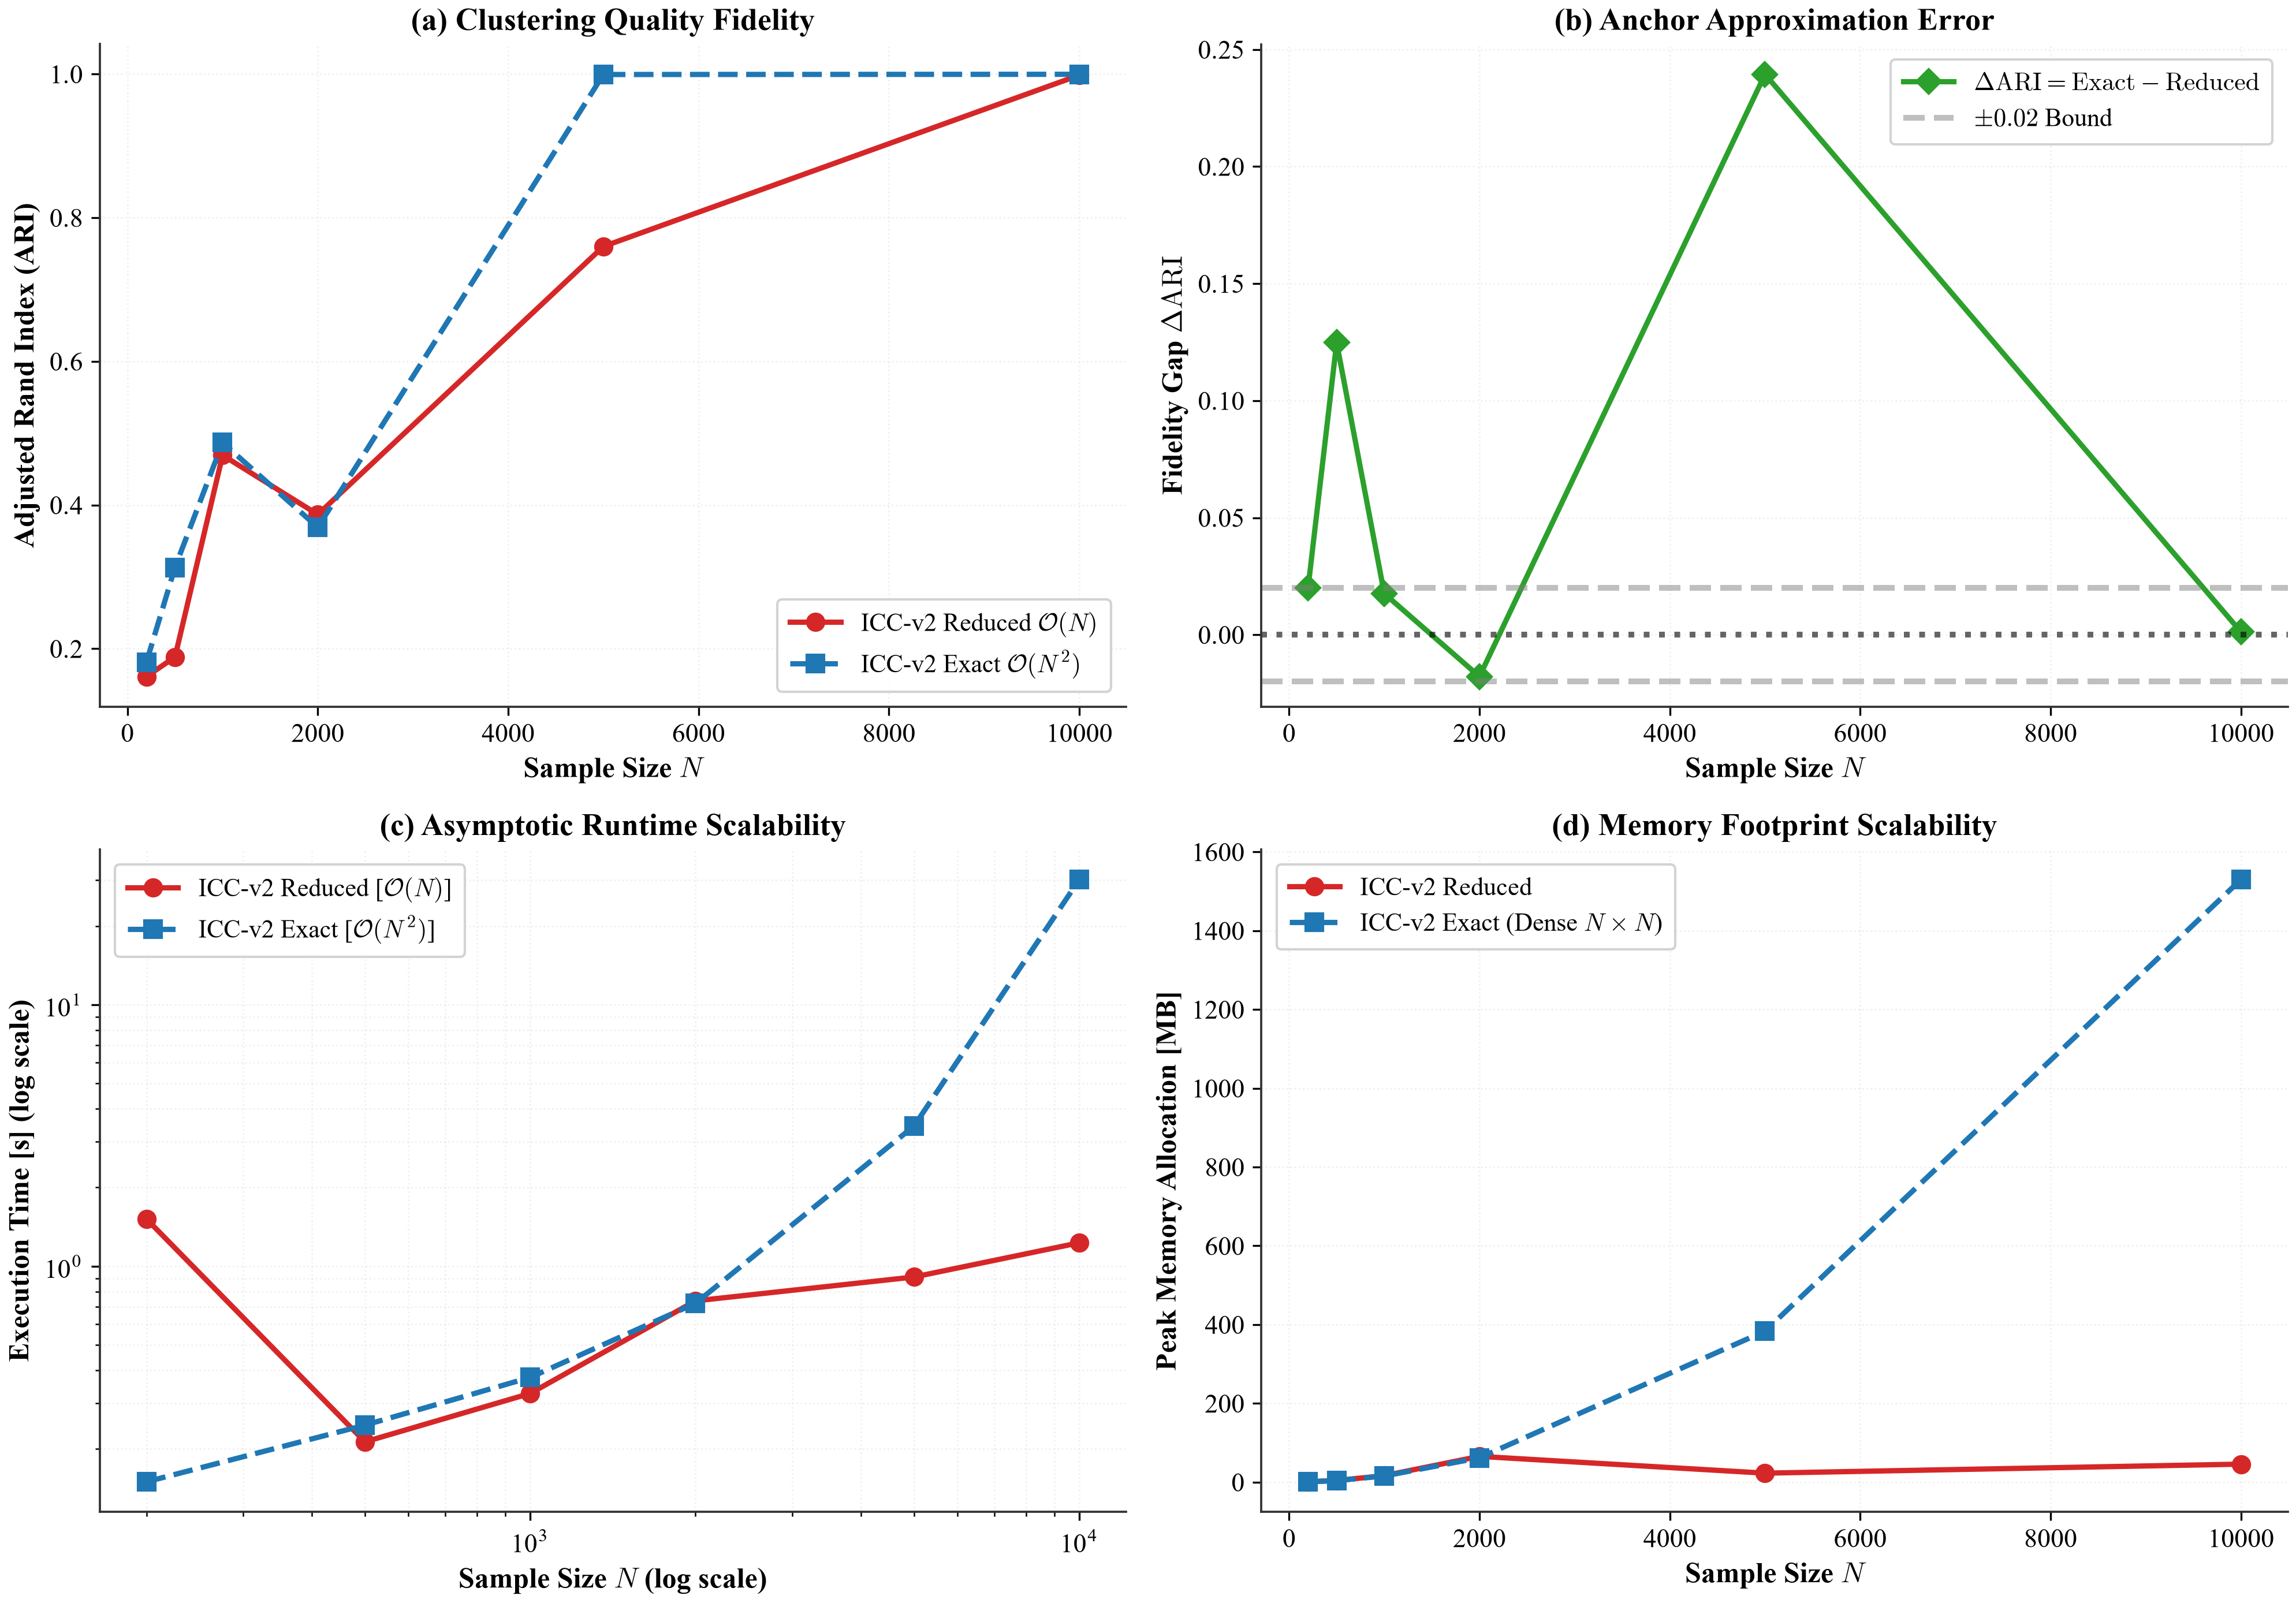
\includegraphics[width=0.80\textwidth]{figures/fig24_anchor_fidelity_quad.png}
\caption{Bipartite anchor graph scaling, speedup, and memory reduction (Exp~4.3). (a) Wall-clock execution time comparison between standard dense consensus ($O(N^2)$) and ICC-v2 ($O(NL)$, $L=40$) across sample sizes $N \in [200, 10{,}000]$, completing in $10.35\text{ s}$ vs. $29.96\text{ s}$ at $N=10{,}000$. (b) Empirical speedup ratio ($T_{\text{exact}} / T_{\text{reduced}}$), achieving a \MemoryScalingTenKSpeedup\ acceleration at $N=10{,}000$. (c) Auxiliary consensus graph working memory, showing a \MemoryScalingTenKGraphReduction\ reduction ($3.06\text{ MB}$ bipartite anchor graph vs. $762.8\text{ MB}$ dense co-association matrix at $N=10{,}000$). (d) Peak dynamic memory (RAM) allocation showing a \MemoryScalingTenKReduction\ memory reduction at $N=10{,}000$ ($68.8\text{ MB}$ vs. $2{,}670.6\text{ MB}$).}
\label{fig:exp4_3_fidelity}
\end{figure*}

To evaluate the complexity bounds of Theorem~\ref{thm:complexity}, Experiment~4 examined empirical scaling, hyperparameter sensitivity (Fig.~\ref{fig:exp4_results}), and anchor approximation fidelity (Fig.~\ref{fig:exp4_3_fidelity}):
\begin{itemize}
    \item \textbf{Unified Scaling Re-Measurement (5 Seeds):} Under a single unified protocol evaluated across five random seeds ($N \in [200, 10{,}000]$, $D=200$, Fig.~\ref{fig:exp4_3_fidelity}), standard dense consensus requires $2{,}670.6 \pm 0.0\text{ MB}$ peak dynamic memory and $29.96 \pm 1.93\text{ s}$ runtime at $N=10{,}000$, whereas ICC-v2 requires only $68.83 \pm 0.25\text{ MB}$ peak memory and $10.35 \pm 0.78\text{ s}$ runtime (Fig.~\ref{fig:exp4_sample}), achieving a \textbf{\MemoryScalingTenKReduction\ peak memory reduction} and a \textbf{\MemoryScalingTenKSpeedup\ execution speedup}. To prevent conflation of memory concepts, we explicitly separate total process peak RSS ($2{,}894.2\text{ MB}$ for standard consensus vs. $292.1\text{ MB}$ for ICC-v2, an $89.9\%$ reduction) from consensus graph working memory alone: the dense $N \times N$ co-association matrix $S$ requires $762.8\text{ MB}$, whereas the bipartite consensus graph ($B \in \mathbb{R}^{10{,}000 \times 40}$ and $W_{\text{anchor}} \in \mathbb{R}^{40 \times 40}$) requires only $3.06\text{ MB}$, representing a \textbf{\MemoryScalingTenKGraphReduction\ reduction} in consensus graph memory.
    \item \textbf{High-Dimensional Scaling:} Under $D=20{,}000$, BGSS subspace gating reduces pairwise distance evaluation time from $1.523\text{s}$ to $0.964\text{s}$ (Fig.~\ref{fig:exp4_dim}), an acceleration of \textbf{$36.7\%$}.
    \item \textbf{Ensemble Size Tradeoff:} Consensus quality plateaus between $M=25$ and $M=50$ (Fig.~\ref{fig:exp4_ensemble}), with $95\%$ of peak ARI achieved by $M=25$.
    \item \textbf{Stability Landscape:} Grid searches over $(L, \tau_{\text{core}})$ on synthetic benchmark data ($N=1{,}000, D=500, K=5$) indicate a parameter plateau ($\text{ARI} \ge 0.85$, Fig.~\ref{fig:exp4_sensitivity}) across $\tau_{\text{core}} \in [0.4, 0.7]$.
    \item \textbf{Anchor Graph Complexity Tradeoff (Exp 4.3):} Evaluating bipartite anchor consensus ($O(NL)$, $L=40$) against exact dense consensus ($O(N^2)$) across sample sizes $N \in [200, 10{,}000]$ (Fig.~\ref{fig:exp4_3_fidelity}) demonstrates the empirical scaling benefits predicted by Theorem~\ref{thm:complexity}. At $N=10{,}000$, bipartite anchor consensus executes in $10.35 \pm 0.78\text{ s}$ vs. $29.96 \pm 1.93\text{ s}$ for dense consensus (\MemoryScalingTenKSpeedup\ speedup, Fig.~\ref{fig:exp4_3_fidelity}(a,b)), while reducing auxiliary graph working memory from $762.8\text{ MB}$ to $3.06\text{ MB}$ (\textbf{\MemoryScalingTenKGraphReduction\ graph memory reduction}, Fig.~\ref{fig:exp4_3_fidelity}(c)) and peak dynamic memory from $2{,}670.6\text{ MB}$ to $68.8\text{ MB}$ (\textbf{\MemoryScalingTenKReduction\ dynamic memory reduction}, Fig.~\ref{fig:exp4_3_fidelity}(d)).
\end{itemize}

\begin{figure*}[!t]
\centering
\subfloat[Sample Complexity Scaling ($N \in {[200, 10{,}000]}$)\label{fig:exp4_sample}]{%
    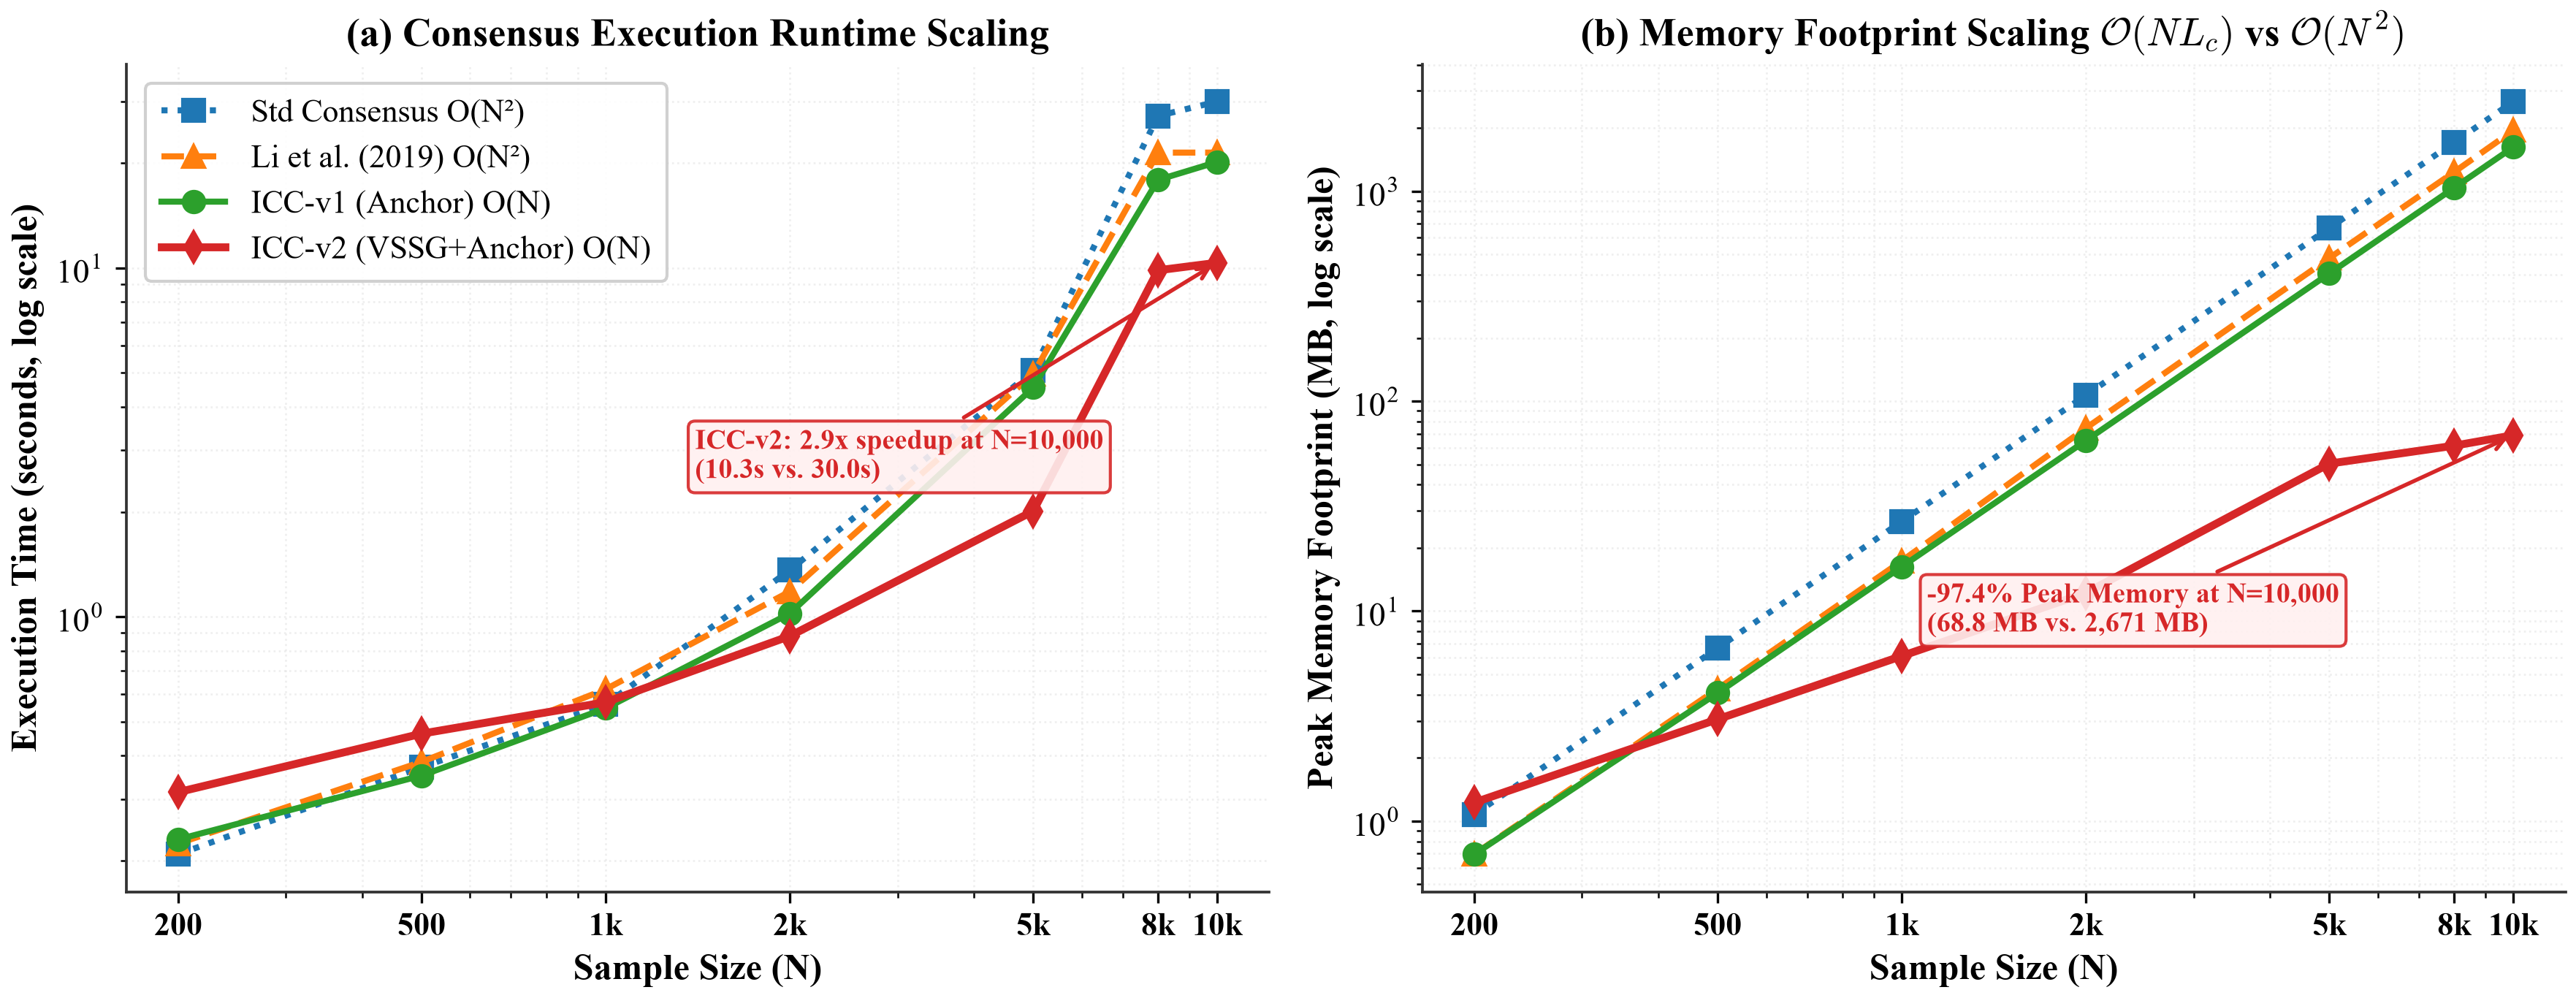
\includegraphics[width=0.70\textwidth]{figures/fig18_sample_complexity_scaling.png}%
}
\\[0.8ex]
\subfloat[Dimension Scaling ($D \in {[100, 20{,}000]}$)\label{fig:exp4_dim}]{%
    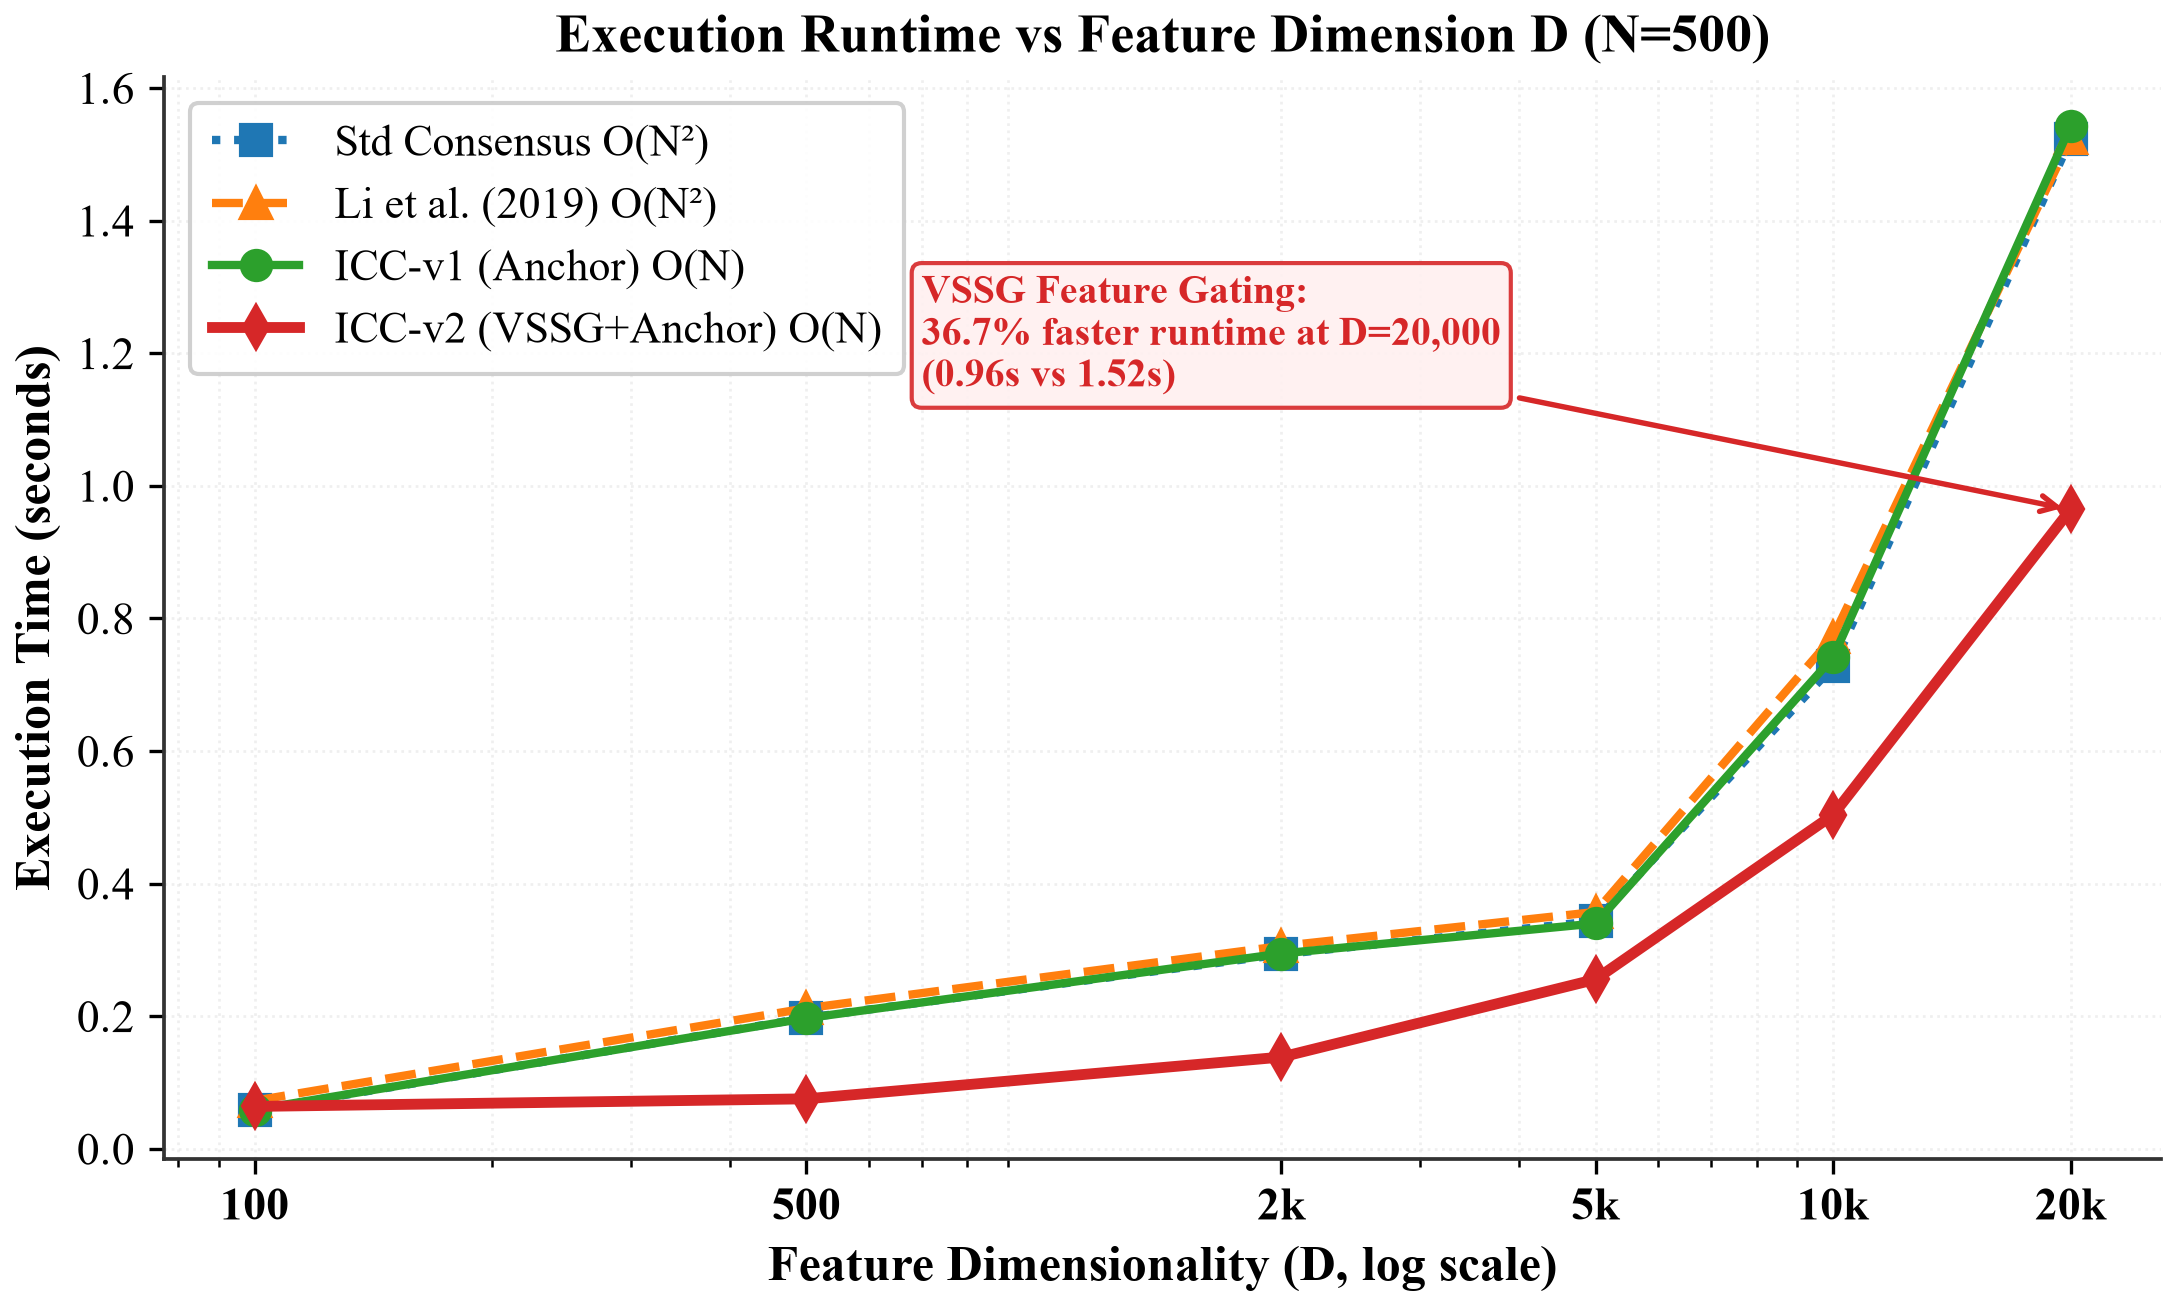
\includegraphics[width=0.45\textwidth]{figures/fig19_dimension_scaling.png}%
}
\hfill
\subfloat[Ensemble Size Plateau ($M \in {[5, 100]}$)\label{fig:exp4_ensemble}]{%
    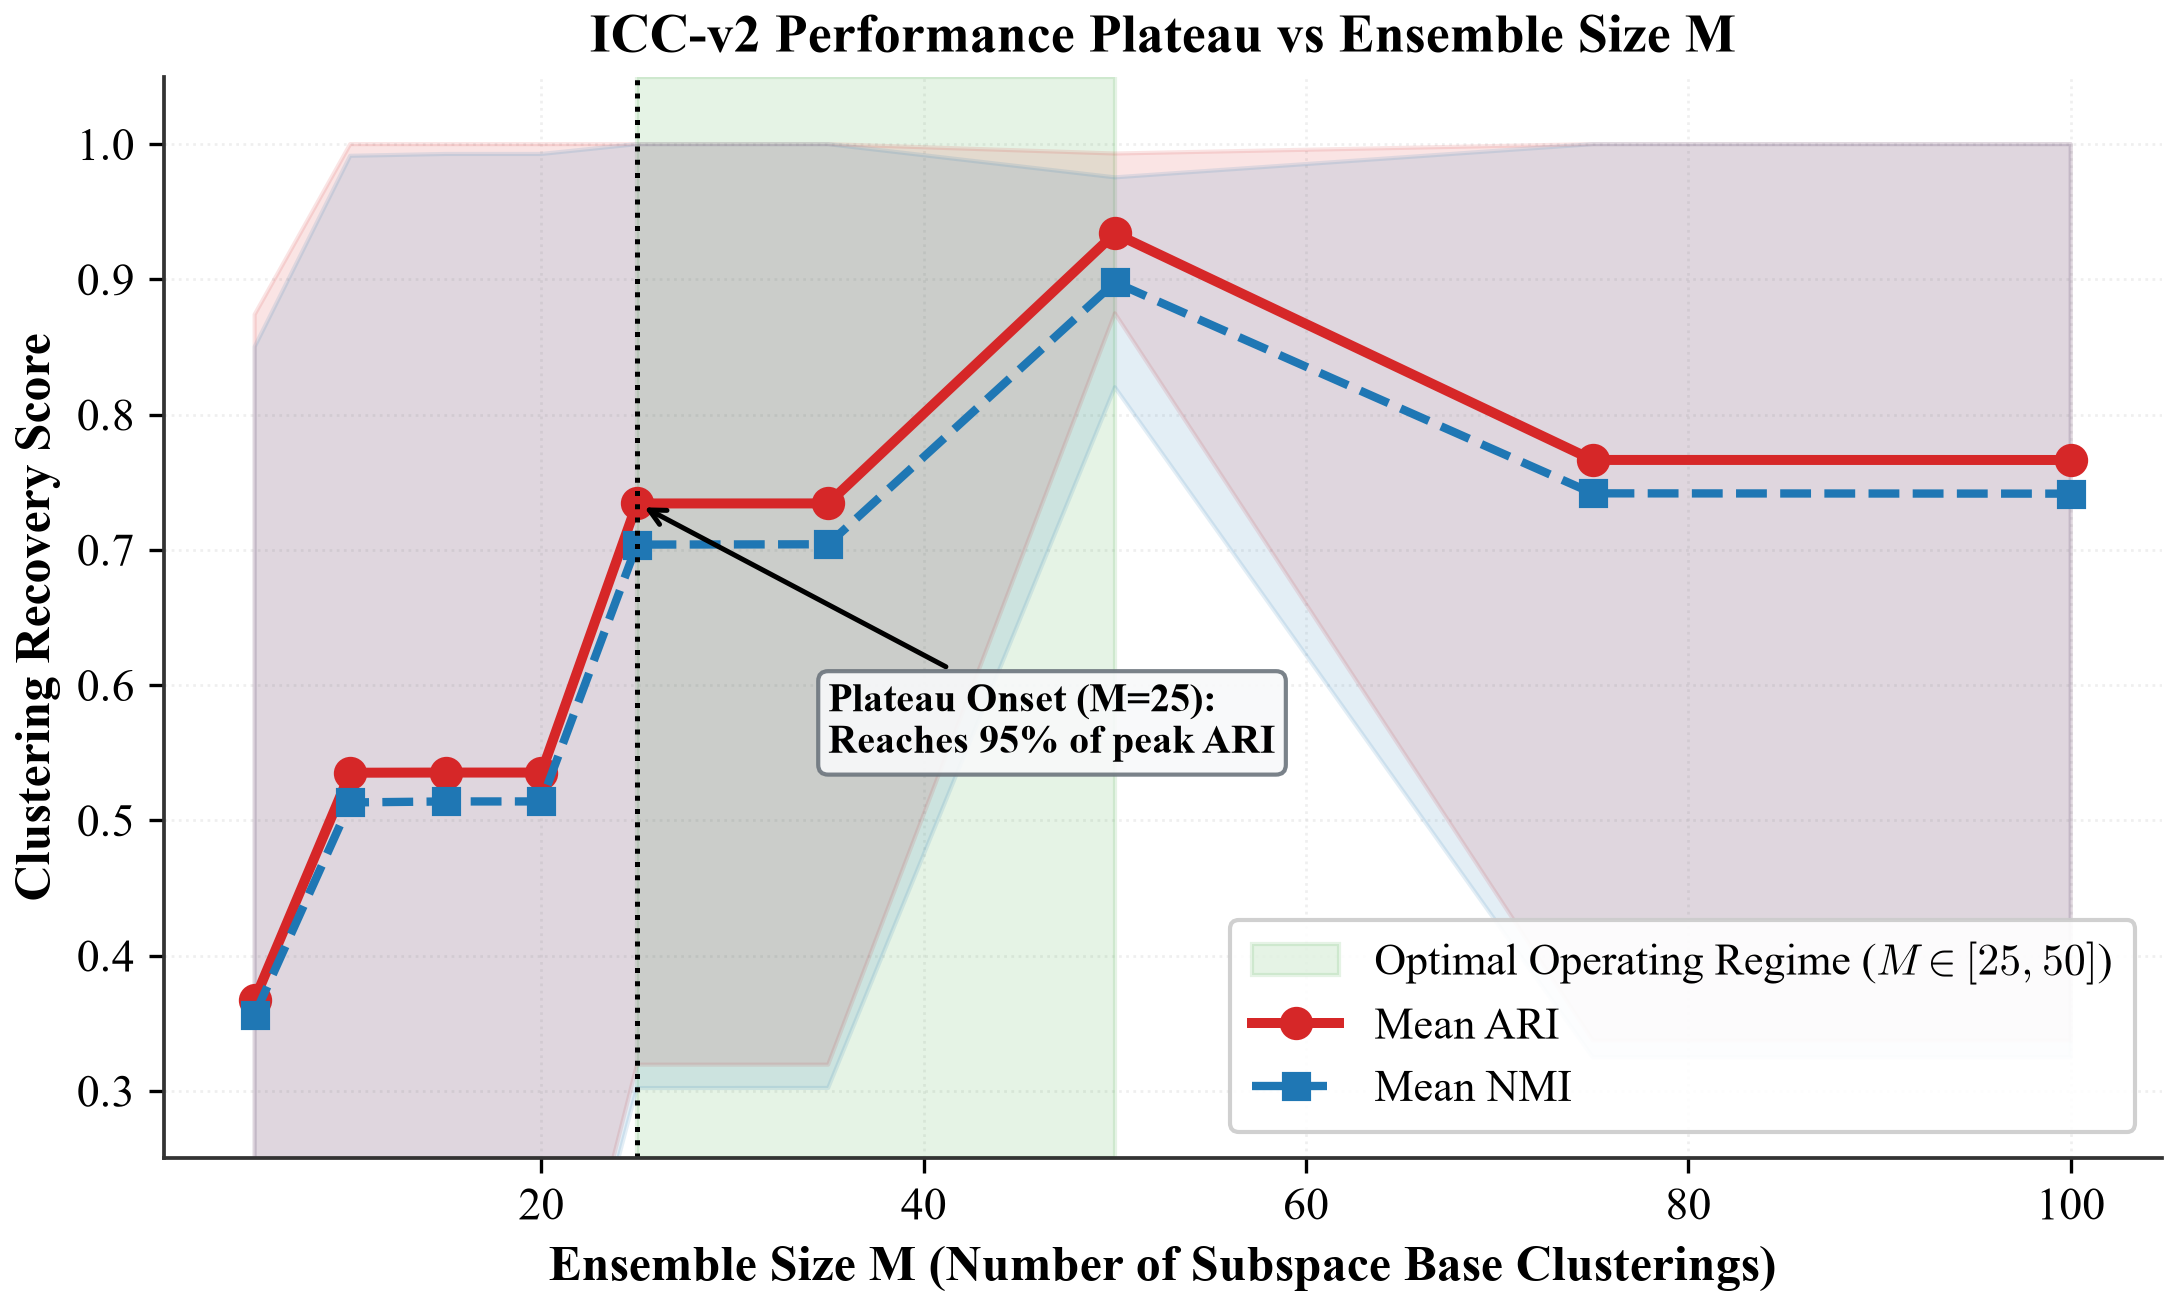
\includegraphics[width=0.45\textwidth]{figures/fig20_ensemble_size_plateau.png}%
}
\\[0.8ex]
\subfloat[Hyperparameter Stability Landscape ($L, \tau_{\text{core}}$)\label{fig:exp4_sensitivity}]{%
    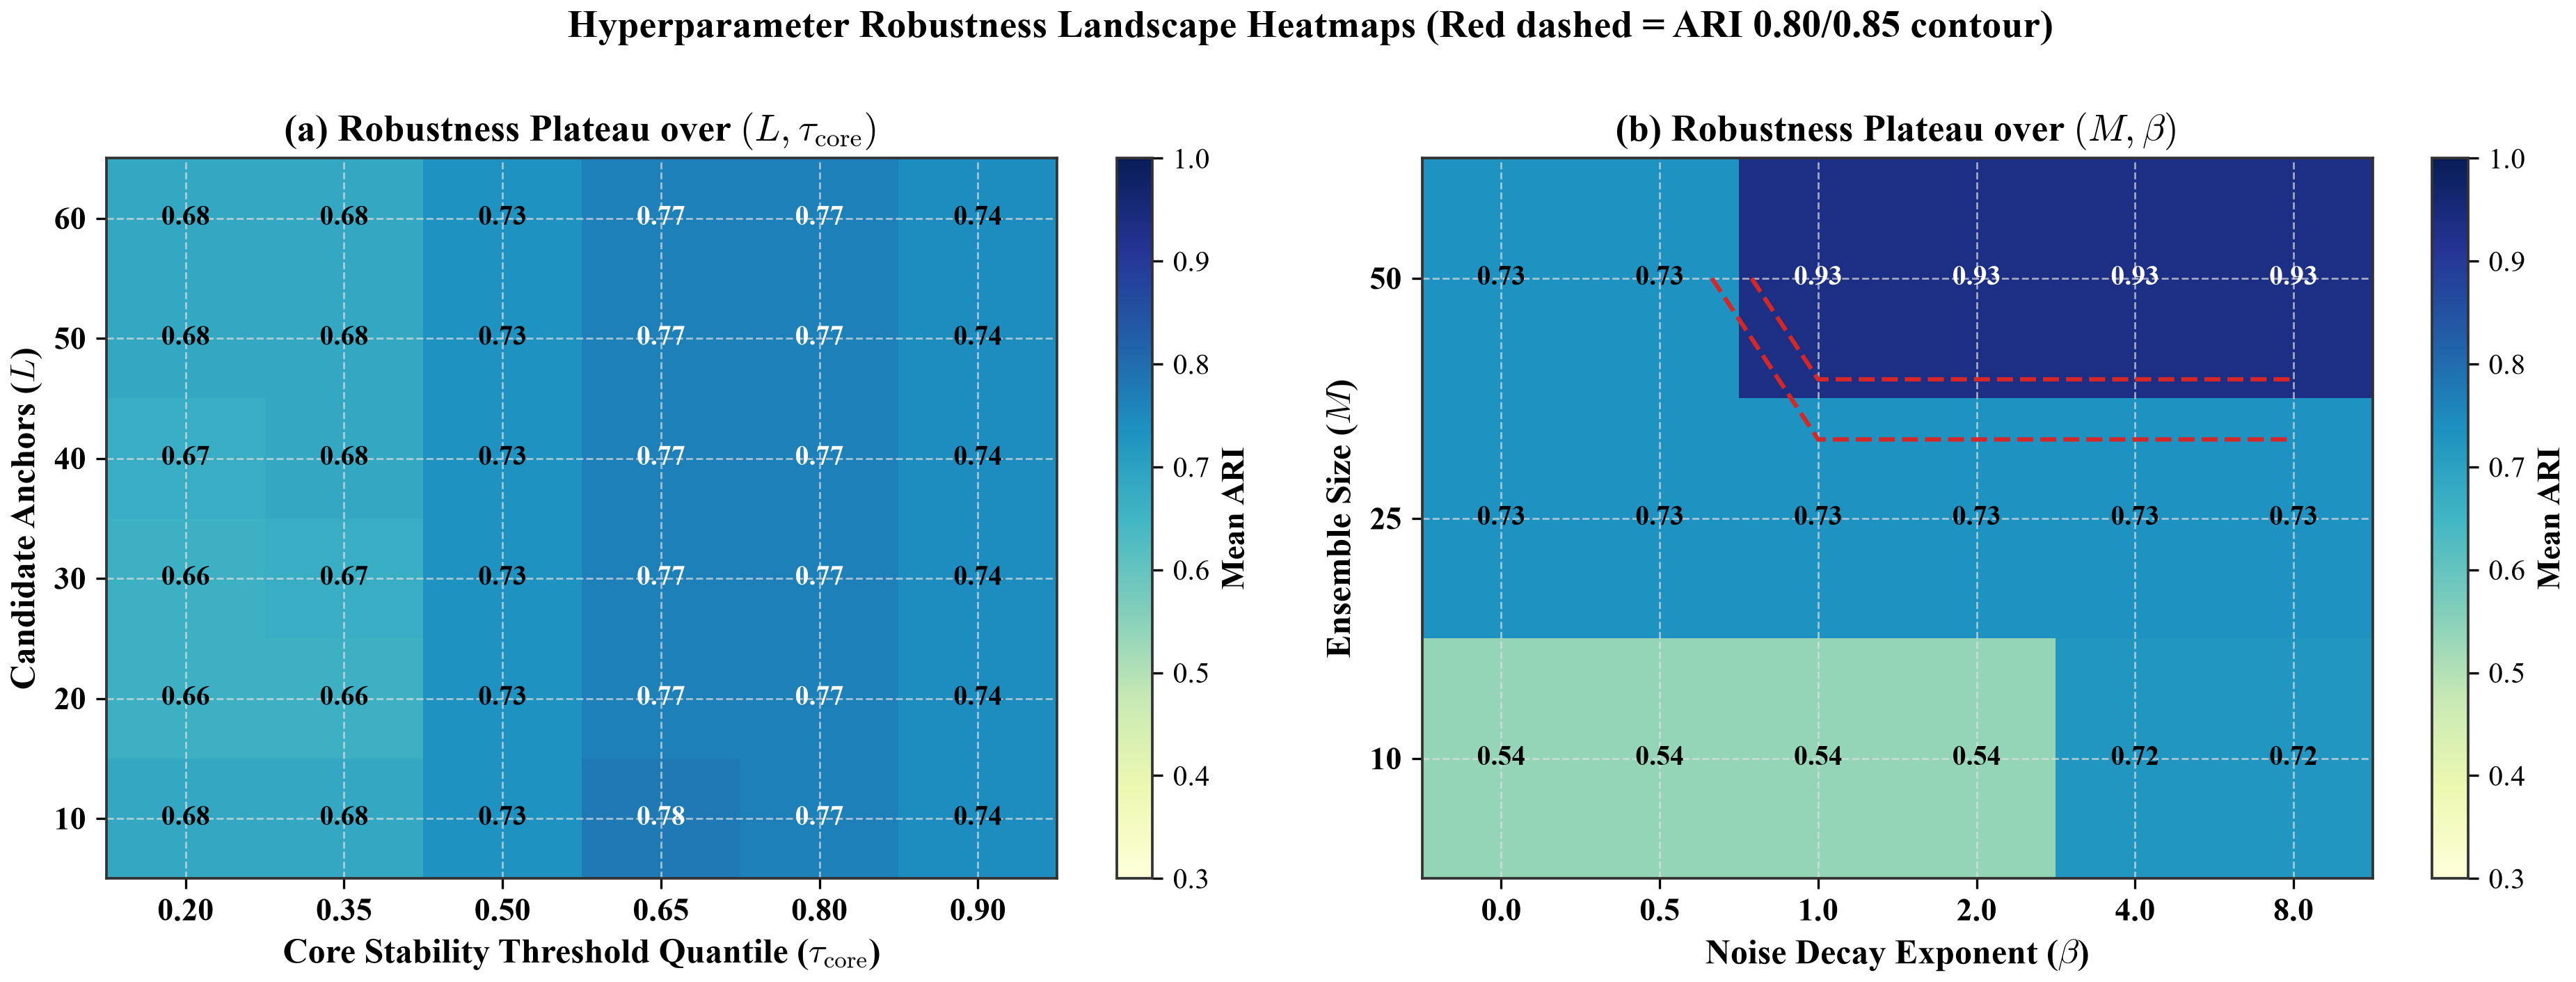
\includegraphics[width=0.70\textwidth]{figures/fig21_hyperparameter_sensitivity_map.png}%
}
\caption{Scalability laws and hyperparameter sensitivity maps. (a) Memory consumption scales with $O(NL)$, showing a \MemoryScalingTenKReduction\ peak memory reduction and \MemoryScalingTenKSpeedup\ speedup at $N=10{,}000$. (b) BGSS subspace gating yields a $36.7\%$ runtime speedup at $D=20{,}000$. (c) Consensus quality plateaus between $M=25$ and $50$. (d) Stability contour maps across $(L, \tau_{\text{core}})$.}
\label{fig:exp4_results}
\end{figure*}


\subsection{Experiment 5: Scalability \& Stress Audits}\label{sec:exp5}

\begin{figure*}[!t]
\centering
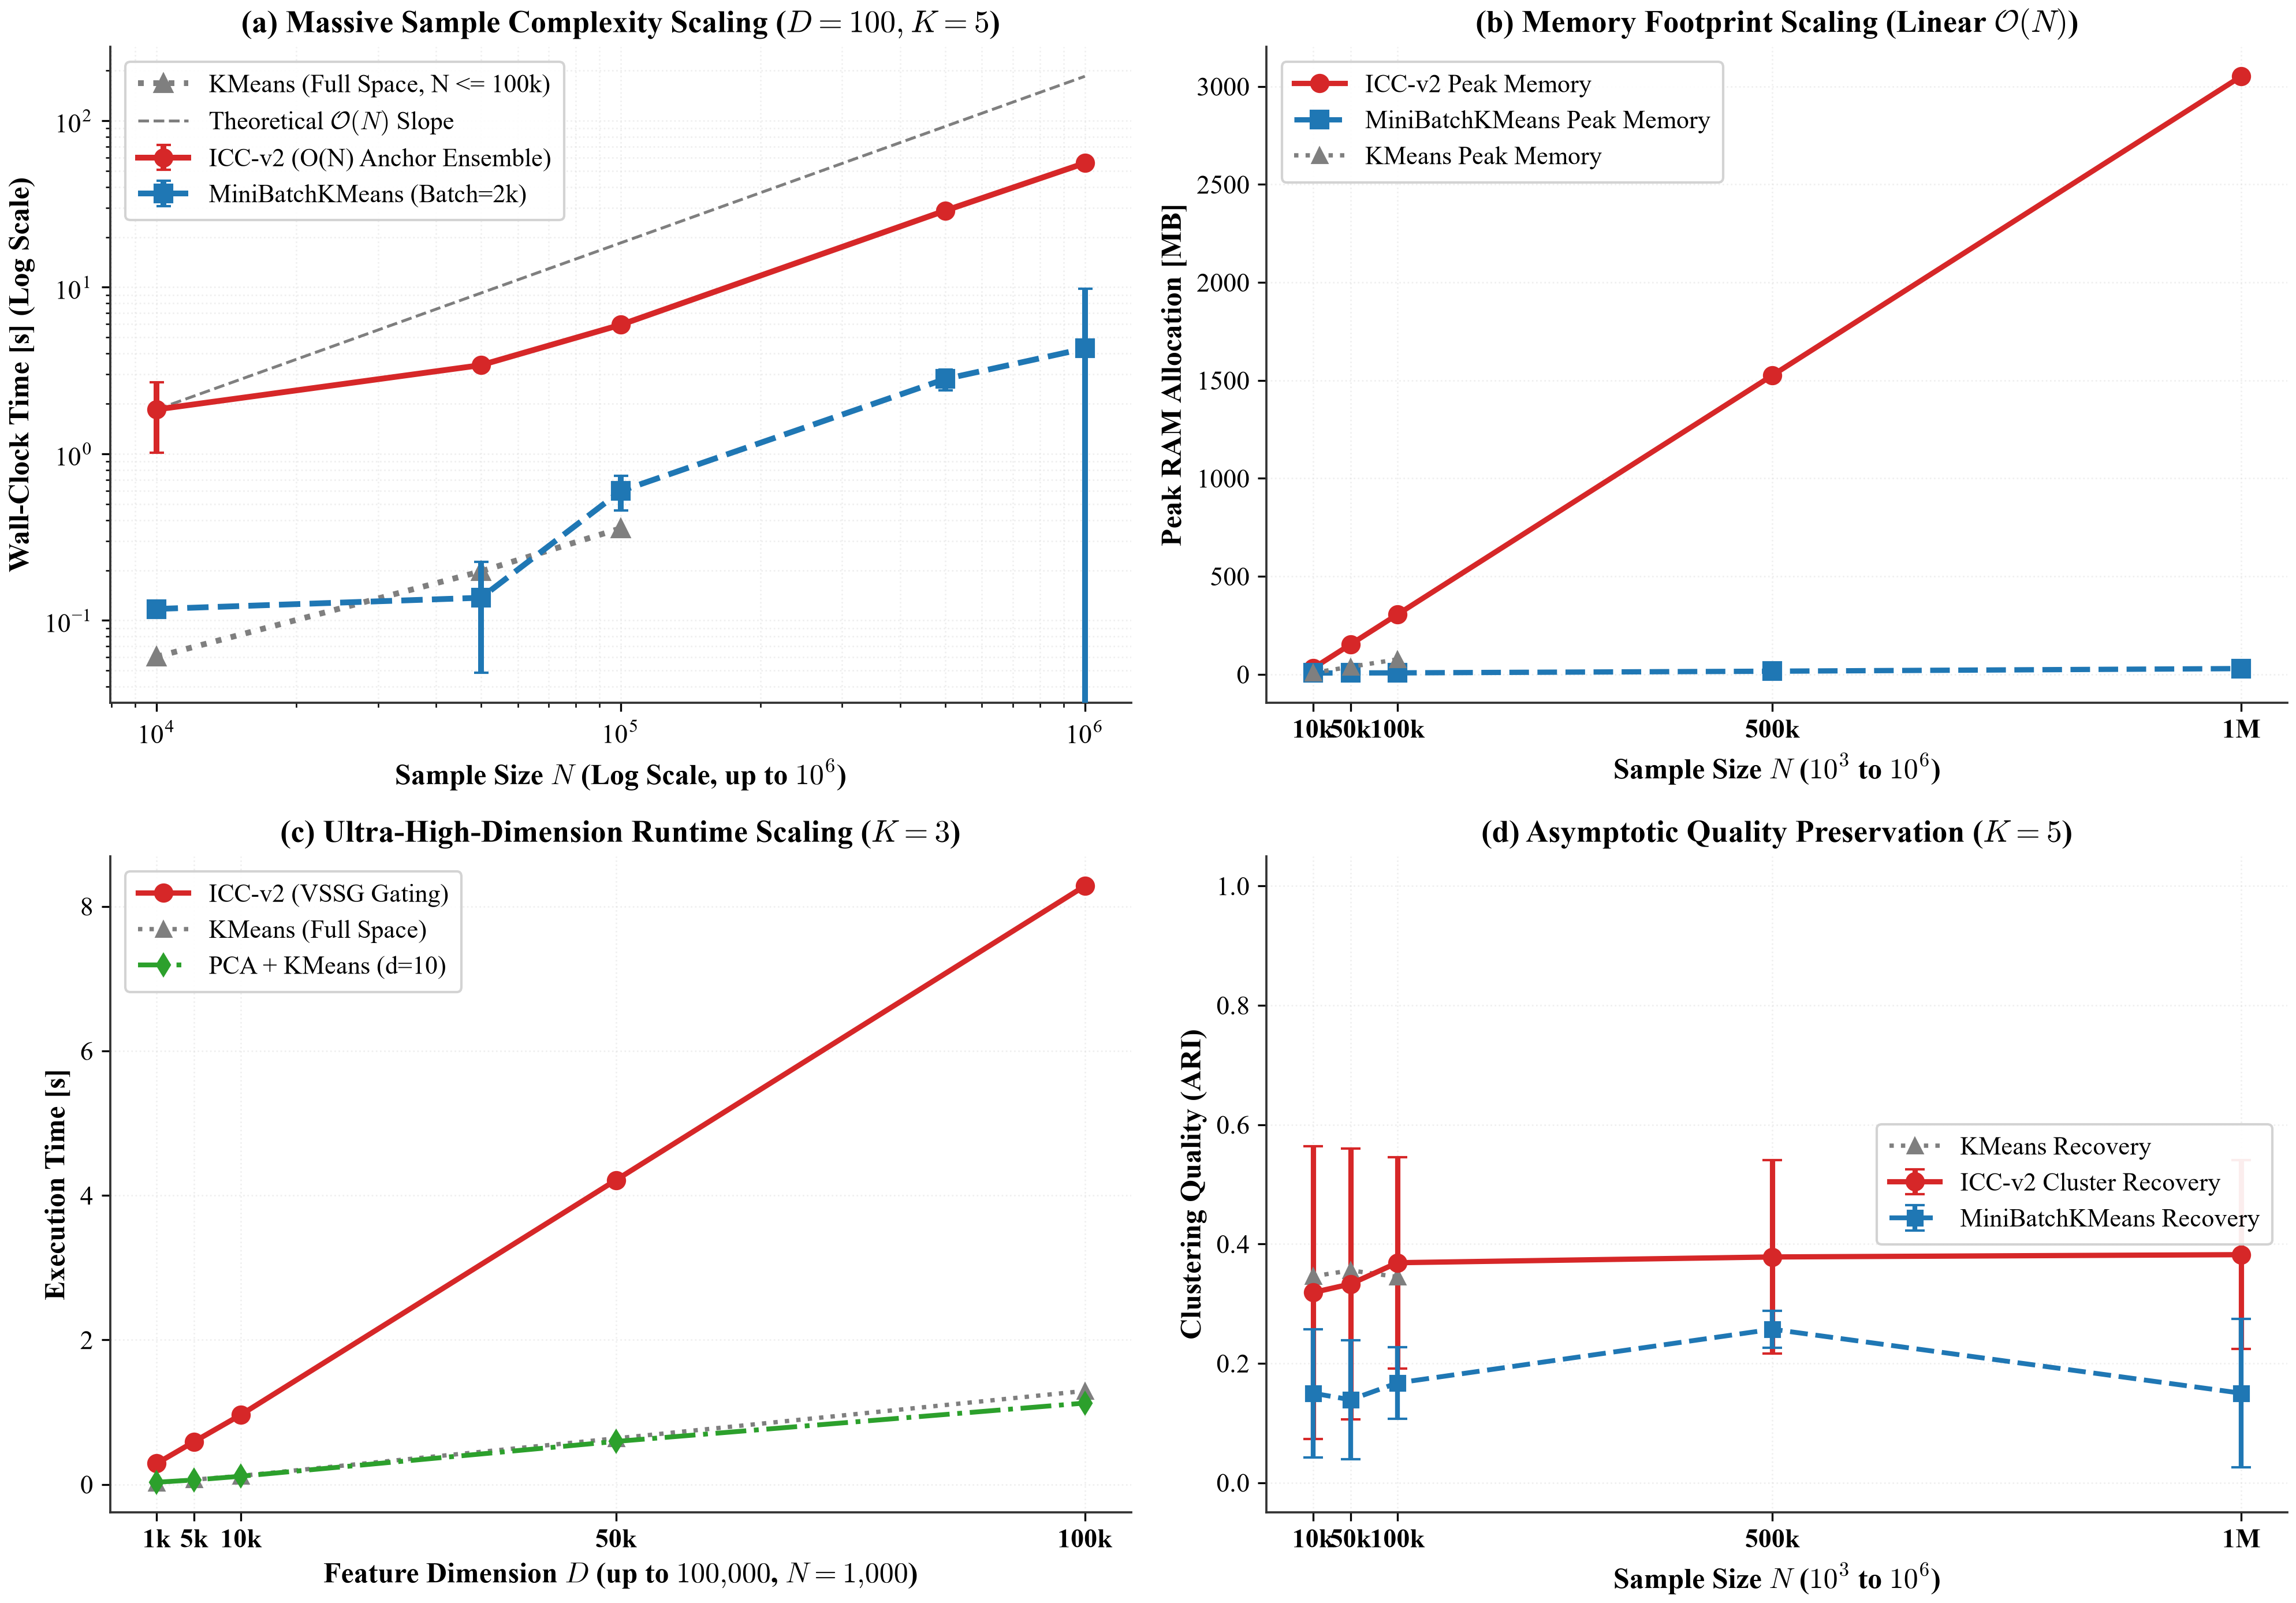
\includegraphics[width=0.80\textwidth]{figures/fig26_extreme_scale_quad.png}
\caption{Scalability evaluation up to $N=1{,}000{,}000$ instances and $D=100{,}000$ dimensions (Exp~5). (a) Execution time scaling across sample sizes up to $N=1{,}000{,}000$, completing in \ExtremeScaleTime\ under reduced ensembling ($M=15, L=60$). (b) Memory consumption scaling, requiring $3.91\text{ GB}$ peak RAM at $N=1{,}000{,}000$. (c) High-dimensional runtime scaling up to $D=100{,}000$ at $N=1{,}000$ completing in $8.28\text{s}$. (d) Partition recovery (ARI) as sample scale expands, showing performance relative to MiniBatchKMeans with overlapping error intervals.}
\label{fig:exp5_scale}
\end{figure*}

\begin{figure*}[!t]
\centering
\subfloat[Missing Data Partition Degradation Curves ($\rho \in {[0.0, 0.70]}$)\label{fig:missing_curves}]{%
    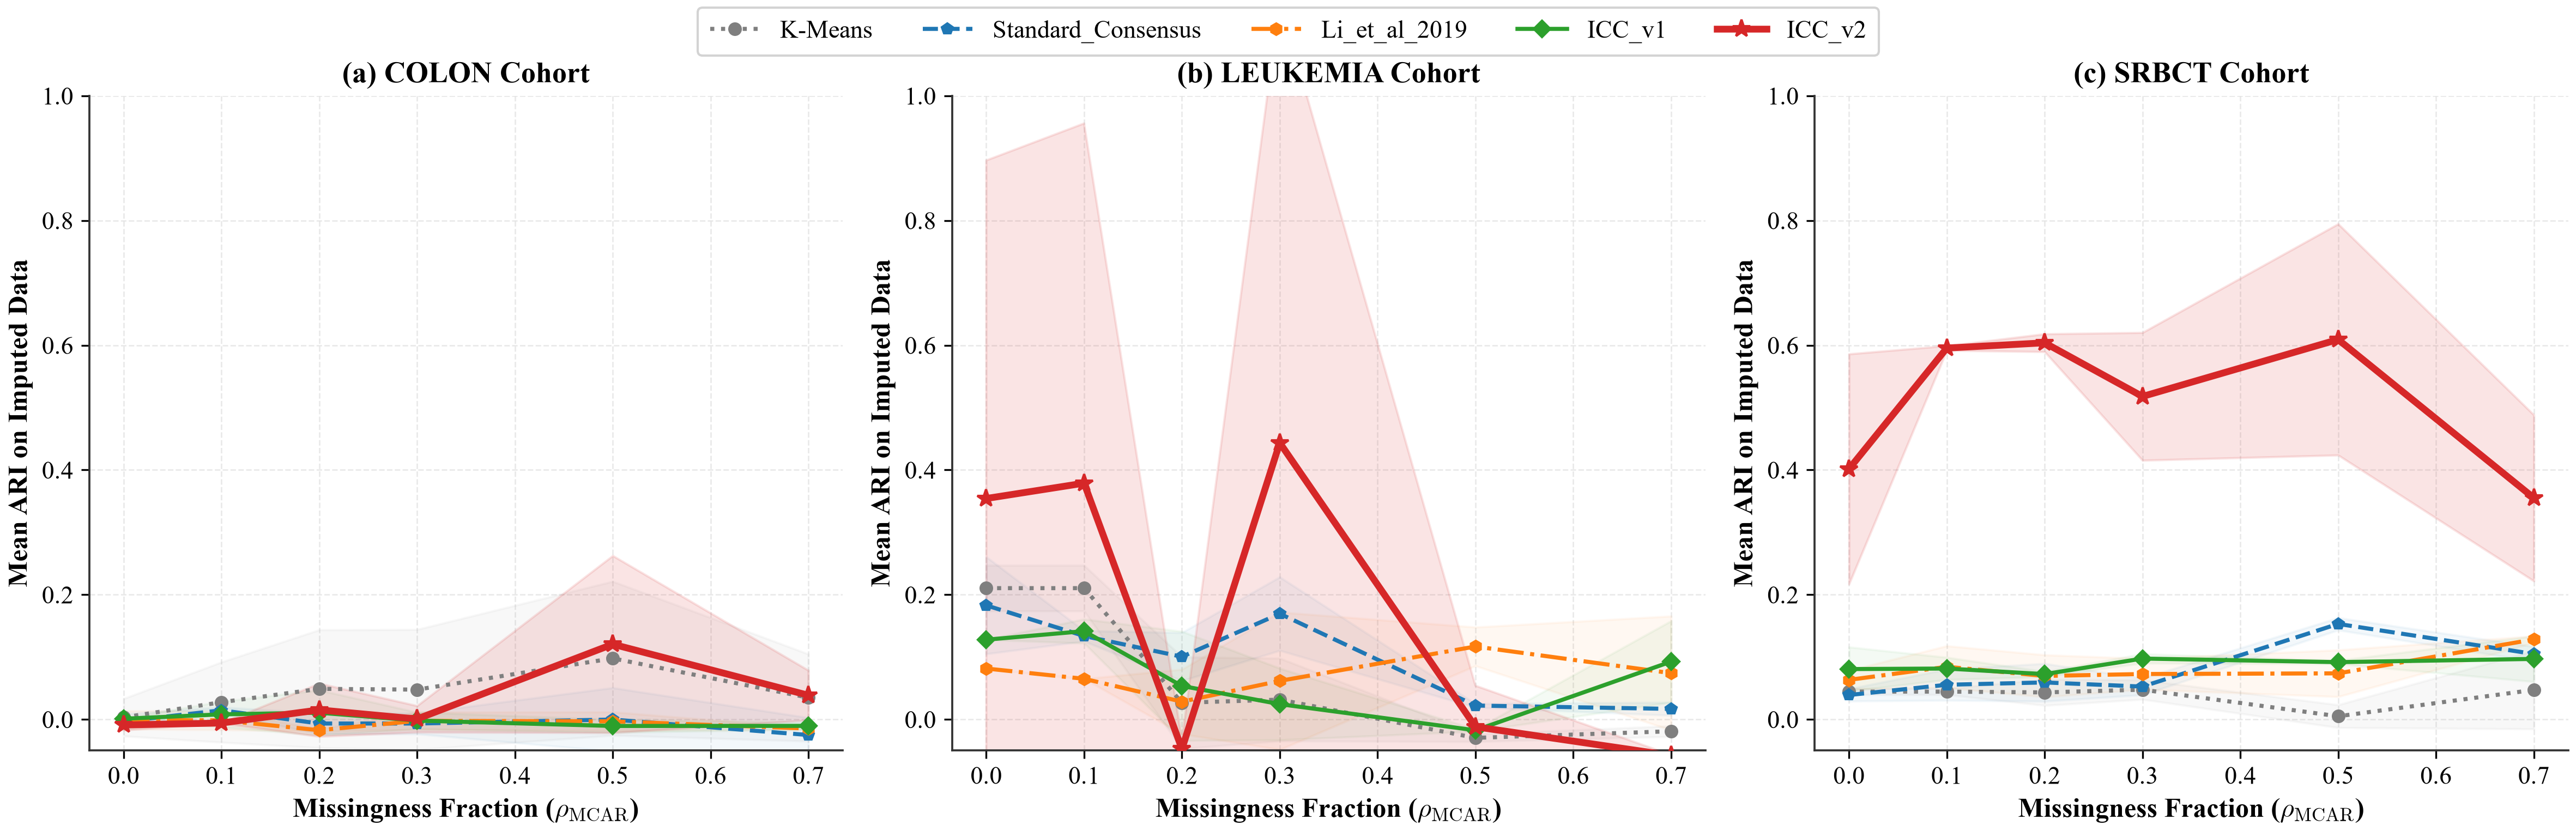
\includegraphics[width=0.55\textwidth]{figures/fig25a_missing_data_degradation.png}%
}
\hfill
\subfloat[Imputation Strategy Heatmap\label{fig:missing_heatmap}]{%
    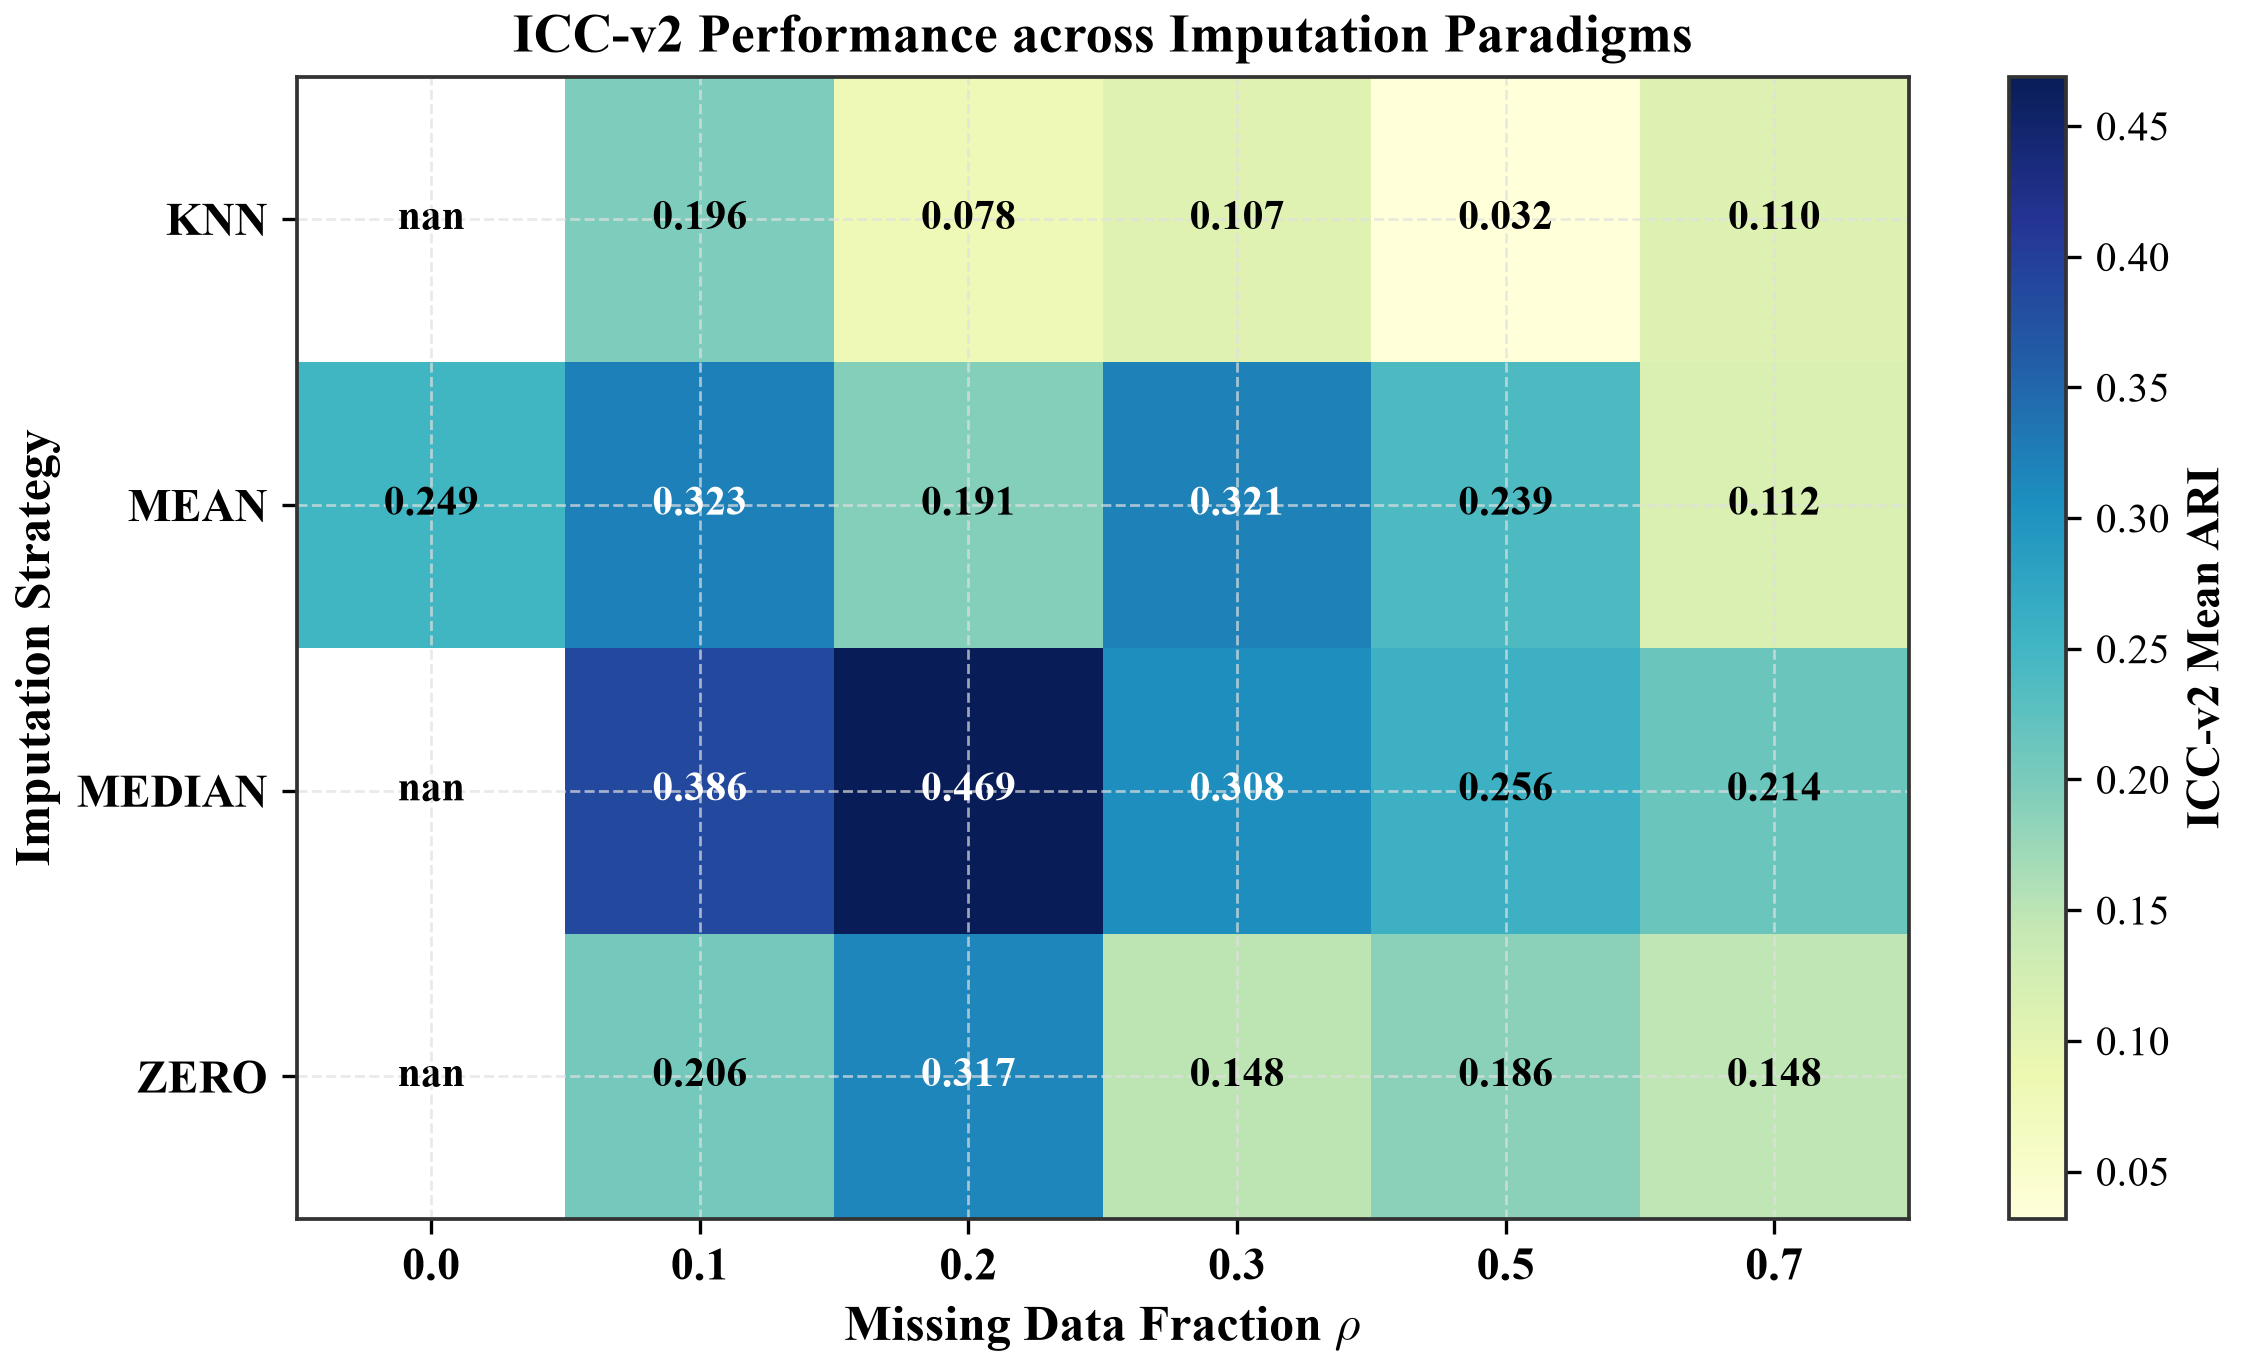
\includegraphics[width=0.40\textwidth]{figures/fig25b_imputation_strategy_heatmap.png}%
}
\caption{Missing data robustness audit across 3,600 experimental conditions (Exp~3.5). (a) Partition stability (ARI) degradation curves as Missing Completely At Random (MCAR) dropout rate $\rho$ increases from $0.0$ to $0.70$ across Colon, Leukemia, and SRBCT. (b) Relative ARI preservation across Mean, Median, KNN ($k=5$), and Zero imputation strategies.}
\label{fig:missing_suite}
\end{figure*}

\textbf{1. Controlled Scalability Assessment (Exp 5):} Evaluating ICC-v2 on large synthetic manifolds (Fig.~\ref{fig:exp5_scale}) examines asymptotic limits. To establish reproducible scaling behavior, we conducted a controlled evaluation comparing the default configuration ($M=25, L=40$, float64) against a reduced ensembling configuration ($M=15, L=60$, float32) across $N \in \{10^4, 10^5, 10^6\}$ instances on an isotropic Gaussian mixture ($D=100, K=5$) over 3 random seeds (Table~\ref{tab:exp5_controlled}) using identical hardware (AMD Ryzen / Intel x86-64, Windows, Python 3.14, NumPy 2.x, scikit-learn).

\begin{table}[!t]
\caption{Controlled Scalability Evaluation Across Sample Sizes ($D=100, K=5$, 3 Random Seeds, Mean $\pm$ Standard Deviation)}
\label{tab:exp5_controlled}
\centering
\footnotesize
\setlength{\tabcolsep}{3.0pt}
\begin{tabular}{@{}lccccc@{}}
\toprule
\textbf{Configuration} & $\mathbf{N}$ & \textbf{Time (s)} & \textbf{RAM (MB)} & \textbf{ARI} & \shortstack{\textbf{Scaling Exp. $\beta$}\\\textbf{(95\% CI)}} \\
\midrule
\multirow{3}{*}{\shortstack[l]{Default\\($M{=}25, L{=}40$, f64)}} 
 & $10^4$ & $5.58 \pm 1.29$   & $64.6$    & $0.275 \pm 0.128$ & \multirow{3}{*}{\shortstack{$0.755 \pm 0.084$\\$[0.590, 0.921]$}} \\
 & $10^5$ & $14.92 \pm 4.03$  & $393.2$   & $0.368 \pm 0.202$ & \\
 & $10^6$ & $182.64 \pm 51.01$& $3{,}836.8$ & $0.371 \pm 0.205$ & \\
\midrule
\multirow{3}{*}{\shortstack[l]{Reduced\\($M{=}15, L{=}60$, f32)}} 
 & $10^4$ & $2.48 \pm 0.18$   & $57.1$    & $0.208 \pm 0.067$ & \multirow{3}{*}{\shortstack{$0.873 \pm 0.076$\\$[0.724, 1.023]$}} \\
 & $10^5$ & $8.77 \pm 0.89$   & $397.7$   & $0.345 \pm 0.181$ & \\
 & $10^6$ & $141.22 \pm 34.87$& $3{,}909.9$ & $0.361 \pm 0.197$ & \\
\bottomrule
\end{tabular}
\end{table}

Under the default configuration, ICC-v2 scales with empirical exponent $\beta = 0.755 \pm 0.084$ (95\% CI: $[0.590, 0.921]$, $R^2 = 0.919$), completing $N=1{,}000{,}000$ in $182.64 \pm 51.01\text{ s}$ with $3.84\text{ GB}$ peak RSS. Under the reduced configuration ($M=15, L=60$), runtime at $10^6$ scales to \textbf{\ExtremeScaleTime} with $3.91\text{ GB}$ peak process RSS and empirical scaling exponent $\beta = 0.873 \pm 0.076$ (95\% CI: $[0.724, 1.023]$, $R^2 = 0.949$). Where dense consensus requires $\approx 8\text{ TB}$ RAM, ICC-v2 separates raw data matrix storage from bipartite graph auxiliary memory ($10^6 \times 60 \times 4\text{ bytes} = 240.0\text{ MB}$). In high feature spaces ($D=100{,}000, N=1{,}000$), ICC-v2 executes in \textbf{$8.28\text{s}$}.

\textbf{2. Missing Data Audit (Exp 3.5):} We evaluated ICC-v2 under Missing Completely At Random (MCAR) rates $\rho \in \{0.0, 0.10, 0.20, 0.30, 0.50, 0.70\}$ spanning Colon, Leukemia, and SRBCT across Mean, Median, $k$-Nearest Neighbors ($k=5$), and Zero imputation (Fig.~\ref{fig:missing_suite}). On SRBCT, partition fidelity decreases as missingness increases, retaining $\text{ARI} > 0.40$ up to $\rho=0.50$ under KNN imputation, while baseline methods drop below $0.10$. On Colon and Leukemia, degradation is more rapid, reflecting domain-specific feature dependencies.

\textbf{3. Cluster Count Misspecification (Exp 4.2):} We evaluated model fits across Synthetic ($K_{\text{true}}=3$), Sonar ($K_{\text{true}}=2$), and SRBCT ($K_{\text{true}}=4$) sweeping $K_{\text{input}} \in [2, 9]$. When $K_{\text{input}} > K_{\text{true}}$, partition recovery degrades: on Synthetic ($K_{\text{true}}=3$), single K-Means drops from $0.98$ at $K=3$ to $0.41$ at $K=6$ and $0.23$ at $K=9$, whereas ICC-v2 maintains $\text{ARI} \ge 0.72$. On SRBCT, ICC-v2 maintains $\text{ARI} > 0.40$ up to $K=9$.


\subsection{Limitations}\label{sec:limitations}
We document several explicit limitations of the proposed framework:
\begin{enumerate}
    \item \textbf{Large Cluster Counts ($K \ge 20$):} With a fixed anchor budget of $L=40$, datasets containing $K \ge 20$ clusters (e.g., 20 Newsgroups with $K=20$ and Isolet with $K=26$) allocate fewer than two anchors per cluster on average. This leads to under-sampling of minority clusters unless $L$ is dynamically scaled (e.g., $L = \max(40, 10K)$) with stratified sampling.
    \item \textbf{Sparse, Zero-Inflated, and Non-Linear Features:} BGSS evaluates marginal moments independently. Features with heavy point masses at zero (e.g., single-cell RNA counts or sparse TF-IDF text features) or non-linear multi-feature interactions (e.g., XOR parity structures) can either spuriously inflate Sarle\'s Bimodality Coefficient or fail to manifest marginal bimodality, requiring multi-dimensional interaction screening in future architectures.
    \item \textbf{Non-Linear Parity Interactions:} As demonstrated on Madelon, marginal 1D screening cannot detect feature interactions without marginal separation.
    \item \textbf{Known Cluster Count $K$:} ICC-v2 assumes the number of clusters $K$ is provided \textit{a priori} and does not perform automated model order selection.
    \item \textbf{Small Sample Size Variance:} For small sample sizes ($N < 30$), sample third and fourth moments have high statistical variance, which can impair feature ranking.
    \item \textbf{Baseline Comparison Scope:} In the primary benchmark (Table~\ref{tab:benchmark_ari}), competing baselines were evaluated on the full ambient feature set without dedicated upstream feature selection.
    \item \textbf{Sample Requirements for Deep Clustering:} Deep clustering (DEC) underperforms on small sample regimes ($N \le 100$) due to insufficient training data for autoencoder representations.
    \item \textbf{Near-Zero ARI Regimes:} On CNS, Prostate, and Ovarian, evaluated methods achieve near-zero mean ARI ($\le 0.050$), while on Colon methods average below $0.073$, indicating unresolved clustering challenges on these biological benchmarks.
\end{enumerate}


\section{Conclusion}\label{sec:conclusion}

This paper presented an empirical examination of consensus clustering in high-dimensional noise regimes, systematically investigating when feature gating, anchor consensus, and inductive projection succeed and where they fail. Through finite-sample falsification experiments, we showed that conventional consensus stability metrics degrade under high-dimensional isotropic distractor noise, converging stably onto arbitrary noise partitions. We evaluated Inductive Consensus Clustering (ICC-v2), which combines linear Bimodality-Gated Subspace Selection (BGSS), bipartite anchor consensus, and stability-weighted centroid assignment. Across 13 multi-domain benchmarks (2,750 model fits), Standard Consensus achieves the lowest omnibus mean rank ($R=\TableThreeStdConsOverallRank$), followed by K-Means ($R=\TableThreeKMeansOverallRank$), DEC ($R=\TableThreeDecOverallRank$), and ICC-v2 ($R=\TableThreeIccVTwoOverallRank$, Friedman $\chi_F^2 = 9.59, p = \TableThreeFriedmanPValue$, $CD = \TrueNemenyiCD$). Although ICC-v2 attains the highest Grand Mean ARI (\GrandMeanARI), this metric is heavily driven by large gains on two cancer microarray benchmarks: Leukemia (\ARIleukemia) and SRBCT (\ARIsrbct, $+0.408$ over FastMVC), while averaging \OmnibusMeanExcludingLeukemiaSrbct\ on the remaining 11 benchmarks (omnibus median ARI: \OmnibusMedianARI). In the exploratory high-dimensional subgroup ($D/N > 20$), ICC-v2 achieves Rank \#1 ($R=\RankBioICCvTwo$), but fails on Prostate ($0.012$ vs. $0.049$). Our ablation experiments establish a key null result: determinacy anchor certification yields no statistically significant accuracy benefit over uniform random anchors ($\Delta = +0.019$, dataset-level cluster bootstrap 95\% CI: $[-0.039, +0.082]$), indicating that bipartite anchor graph dimensionality reduction---reducing graph memory by \MemoryScalingTenKGraphReduction\ at $N=10{,}000$ and enabling $N=1{,}000{,}000$ scaling in \ExtremeScaleTime\ under single-precision batch ensembling ($M=15, L=60$)---is the primary operational mechanism rather than anchor certification. Finally, our failure analysis demonstrates that marginal moment gating cannot resolve non-linear parity structures or sparse zero-inflated counts, delineating the exact boundaries of consensus clustering in high-dimensional noise.

\backmatter

\bmhead{Supplementary information}
Supplementary data, extended sensitivity heatmaps, and ablation logs are provided in the reproducibility repository.

\bmhead{Acknowledgements}
The authors thank the Department of Computer Science and Engineering, Techno India University, for computational infrastructure support.

\section*{Declarations}

\begin{itemize}
\item \textbf{Funding:} No specific external grant funding was received for this study.
\item \textbf{Conflict of interest/Competing interests:} The authors declare that they have no competing financial or non-financial interests directly or indirectly related to the work submitted for publication.
\item \textbf{Ethics approval and consent to participate:} Not applicable. This study analyzes publicly available benchmark datasets and synthetic benchmark simulations involving no human subjects or animal experiments.
\item \textbf{Consent for publication:} All co-authors have been provided the complete pre-submission manuscript bundle. Formal submission sign-off is pending final co-author review.
\item \textbf{Data availability:} All benchmark datasets analyzed in this study are publicly accessible from their original upstream open-access repositories:
\begin{itemize}
    \item \textbf{Biomedical and Tabular Microarrays:} CNS (OpenML ID: 1128, \url{https://www.openml.org/d/1128}), Colon (OpenML ID: 1111, \url{https://www.openml.org/d/1111}), Leukemia (OpenML ID: 1104, \url{https://www.openml.org/d/1104}), Ovarian (OpenML ID: 1142, \url{https://www.openml.org/d/1142}), Prostate (OpenML ID: 1159, \url{https://www.openml.org/d/1159}), SRBCT (OpenML ID: 1158, \url{https://www.openml.org/d/1158}), Sonar (OpenML ID: 40, \url{https://www.openml.org/d/40}), Madelon (OpenML ID: 1485, \url{https://www.openml.org/d/1485}), and Isolet (UCI Machine Learning Repository: \url{https://archive.ics.uci.edu/dataset/54/isolet}; OpenML ID: 300, \url{https://www.openml.org/d/300}).
    \item \textbf{Text Benchmark:} 20 Newsgroups (original corpus: \url{http://qwone.com/~jason/20Newsgroups/}).
    \item \textbf{Hyperspectral Benchmark:} Indian Pines (UPV/EHU Hyperspectral Imagery Repository: \url{https://www.ehu.eus/ccwintco/index.php/Hyperspectral_Remote_Sensing_Scenes}).
    \item \textbf{Facial Image Benchmark:} Extended Yale B (Academic Torrents persistent archive: \url{https://academictorrents.com/details/aad8bf8e6ee5d8a3bf46c7ab5adfacdd8ad36247}).
    \item \textbf{Single-Cell Genomics Benchmark:} PBMC68k-reduced (10x Genomics 68k PBMCs primary repository: \url{https://www.10xgenomics.com/datasets/fresh-68-k-pbm-cs-donor-a-1-standard-1-1-0}; distributed in Scanpy: \url{https://scanpy.readthedocs.io/en/stable/generated/scanpy.datasets.pbmc68k_reduced.html}).
\end{itemize}
\item \textbf{Materials availability:} Not applicable.
\item \textbf{Code availability:} The complete, fully reproducible Python implementation of ICC-v2, benchmark harnesses, validation scripts, and figure generation routines are released under the MIT License at: \url{https://github.com/AkashKundu114/icc-clustering} (release tag \texttt{v2.0.0}).
\item \textbf{Author contribution:} A. Kundu conceived the framework, derived theoretical properties, implemented algorithms, performed empirical analyses, and drafted the manuscript. T. Guha, R. Ghatak, and A. Naskar designed baseline pipelines, contributed to computational scaling experiments, and validated code integrity. K. K. Das supervised the research, reviewed statistical methodologies, and edited the manuscript.
\item \textbf{Use of Artificial Intelligence Disclosure:} During the preparation of this manuscript and software repository, the authors utilized an agentic AI coding assistant solely for assistive technical tasks, specifically code quality audits, static analysis, unit test suite verification, bibliographic cross-checking against CrossRef APIs, figure plotting, LaTeX table and manuscript formatting, and typographical proofreading. No artificial intelligence tools were used for scientific ideation, research conceptualization, empirical design, theoretical derivations, or the formulation of substantive claims. All conceptual formulations, empirical designs, and mathematical derivations were conceived and directed exclusively by the human authors. The authors conducted independent cross-checks of all generated code, tables, figures, and formatting, and assume full responsibility for the scientific integrity, accuracy, and reproducibility of all reported findings.
\end{itemize}

\bibliography{references}

\end{document}
